\PassOptionsToPackage{table}{xcolor} 

\documentclass[manuscript,screen]{acmart}
\usepackage{geometry}
\usepackage{fancyhdr}
\usepackage{todonotes}
\usepackage{amsmath}
\usepackage{mathtools}
\usepackage{listings}
\usepackage{tcolorbox}
\usepackage{hyperref}
\usepackage{tabularx}
\usepackage[capitalise]{cleveref}
\crefformat{section}{#2\S#1#3} 
\crefformat{subsection}{#2\S#1#3}
\crefformat{subsubsection}{#2\S#1#3}
\crefformat{figure}{#2Fig. #1#3}
\crefformat{table}{#2Table #1#3}

\usepackage[labelformat=simple]{subcaption}
\renewcommand\thesubfigure{(\alph{subfigure})}  
\usepackage{multirow}
\usepackage{siunitx}
\usepackage{makecell}
\usepackage{pgf}
\usepackage{pgfplots}
\pgfplotsset{compat=1.18}
\usepackage{url}
\setuptodonotes{inline}

\usepackage{tikz}   
\newcommand{\CRicon}[1]{
	\tikz[baseline=(char.base)]{
		\node[shape=circle, rounded corners=3pt, inner sep=0pt,
		top color=black, bottom color=black, text=white,
		font=\bfseries] (char)
		{#1};
	}
}

\usepackage{circledsteps}
\newcommand\myCircled[2][]{\ifmmode
\Circled[fill color=black,inner color=white,#1]{\mathsf{#2}}
\else
\Circled[fill color=black,inner color=white,#1]{\sffamily#2}
\fi
}



\geometry{a4paper, margin=1in}
\setlength{\parskip}{1em}
\setlength{\parindent}{0em}


\pagestyle{fancy}
\fancyhf{}
\fancyhead[L]{SPP 2377 Collaboration}
\fancyhead[R]{\thepage}
\fancyfoot[C]{Draft}


\newtcolorbox{insightbox}{
    colback=purple!10, colframe=purple!80,
    title=Insight:, fonttitle=\bfseries, sharp corners,
    top=2mm, bottom=2mm, left=1mm, right=1mm
}


\lstset{
    basicstyle=\ttfamily\footnotesize,
    breaklines=true,
    frame=single,
    backgroundcolor=\color{gray!10},
    keywordstyle=\color{blue},
    commentstyle=\color{gray},
    stringstyle=\color{red}
}

\newcommand\lk[1]{{\color{magenta!100}{\textbf{Lokesh}:} #1}}
\newcommand\yc[1]{{\color{purple!60}(\textbf{Tony}: #1)}}
\newcommand\ts[1]{{\color{green!60!black}(\textbf{Tristan}: #1)}}
\newcommand\nw[1]{{\color{blue!30!black}(\textbf{Nils FAU}: #1)}}
\newcommand\nils[1]{{\color{blue!80!blue}(\textbf{Start Nils}: #1 :\textbf{EndNils})}}
\newcommand{\ali}[1]{{\itshape\color{teal}\textbf{ALI:~}#1}}
\newcommand{\jp}[1]{{\color{olive}\textbf{Joao:~}#1}}
\newcommand{\as}[1]{{\color{red}\textbf{Asif:~}#1}}
\definecolor{asparagus}{rgb}{0.53, 0.66, 0.42}
\newcommand{\jc}[1]{{\color{asparagus}\textbf{Jeronimo:~}#1}}


\newcommand\bg[1]{{\color{red!60}(Background $\rightarrow$#1$\leftarrow$)}}
\newcommand\cs[1]{{\color{green!60}(Case Study $\rightarrow$#1$\leftarrow$)}}

\author{Yun-Chih Chen}
\author{Tristan Seidl}
\author{Nils Hölscher}
\author{Christian Hakert}
\author{Minh Duy Truong }
\author{Jian-Jia Chen}
\authornote{These authors contributed equally to this work.}
\affiliation{
  \institution{TU Dortmund University}
  \city{Dortmund}
  \country{Germany}
}
\email{{yunchih.chen, tristan.seidl, nils.hoelscher, minhduy.truong, jian-jia.chen}@tu-dortmund.de}

\author{João Paulo C. de Lima\textsuperscript{$\dagger$}}
\author{Asif Ali Khan}
\author{Jeronimo Castrillon\textsuperscript{$\dagger$}}
\authornotemark[1]
\affiliation{
  \institution{Technische Universität Dresden, ScaDS.AI\textsuperscript{$\dagger$}}
  \city{Dresden}
  \country{Germany}
}
\email{{joao.lima, asif_ali.khan, jeronimo.castrillon}@tu-dresden.de}

\author{Ali Nezhadi}
\author{Lokesh Siddhu}
\author{Hassan Nassar}
\author{Mahta Mayahinia}
\author{Mehdi Baradaran Tahoori}
\author{Jörg Henkel}
\authornotemark[1]
\affiliation{
  \institution{Karlsruhe Institute of Technology (KIT)}
  \city{Karlsruhe}
  \country{Germany}
}
\email{{ali.nezhadi, lokesh.siddhu, hassan.nassar, mahta.mayahinia, mehdi.tahoori,henkel}@kit.edu}

\author{Nils Wilbert}
\author{Stefan Wildermann}
\author{Jürgen Teich}
\authornotemark[1]
\affiliation{
  \institution{Friedrich-Alexander-Universität Erlangen-Nürnberg}
  \city{Erlangen}
  \country{Germany}
}
\email{{nils.wilbert, stefan.wildermann, juergen.teich}@fau.de}

\begin{document}


\title{Modeling and Simulating Emerging Memory Technologies: A Tutorial}
\maketitle
\renewcommand{\shortauthors}{Y. Chen et al.}
\authornote{These authors contributed equally to this work.}

\section*{Abstract}
Non-volatile Memory (NVM) technologies present a promising alternative to traditional volatile memories such as SRAM and DRAM. Due to the limited availability of real NVM devices, simulators play a crucial role in architectural exploration and hardware-software co-design. This tutorial presents a simulation toolchain through four detailed case studies, showcasing its applicability to various domains of system design, including hybrid main-memory and cache, compute-in-memory, and wear-leveling design. These case studies provide the reader with practical insights on customizing the toolchain for their specific research needs. The source code is open-sourced.



\section{Introduction}\label{sec:Introduction}
As semiconductor technology advances, energy efficiency is becoming a significant barrier to scalability.
This challenge has resulted in the development of heterogeneous computing devices and the \textit{Dark Silicon} phenomenon, in which portions of a chip are selectively turned off to save energy.
Non-volatile memory (NVM) technologies are a promising solution because they provide energy-efficient alternatives to traditional volatile memory.
Historically confined to storage applications such as SSDs and read-only instruction storage in embedded systems, new NVM technologies with access latencies approaching those of DRAM \cite{pcm:2024, 10145822} have opened the door for their use as main memory with a moderate performance penalty.

However, diverse application contexts expose different design requirements.
On the one hand, small and remote devices (e.g., edge servers at traffic lights or base stations in hard-to-access locations) may operate for extended durations with limited maintenance. In these settings, high power consumption, frequent dirty data writebacks, and costly data restoration upon wake-up are especially problematic for current memory technologies, including DRAM, SSD, and eFlash~\cite{8351201}.
On the other hand, data-center workloads continue to grow in scale and complexity, pushing SRAM and DRAM to their limits in terms of performance, bandwidth, density, and energy usage. 
This has driven the evolution of memory technology toward greater heterogeneity and specialization.
NVMs, with their longer retention times, are well-positioned to play an important role in this transition, particularly as an adaptable, energy-efficient memory option for a broader spectrum of applications, ranging from power-constrained wearable devices up to large-scale enterprise systems.


However, to fully realize NVMs' potential in mainstream computing, extensive research in computer architecture is required to address their challenges
, including limited endurance, higher fault rates, and expensive write operations.
These characteristics necessitate adaptive hardware-software co-design solutions to improve performance and longevity.
Effective co-design strategies must align software requirements with hardware limitations using techniques such as wear leveling, error correction, and vertical integration, ensuring that both software and hardware work together to maximize NVMs' capabilities.

Recognizing the importance of addressing these challenges as part of a broader effort to advance memory technologies, the German Research Foundation (DFG) launched SPP 2377 in 2022.
This 6-year national priority program brings together 23 principal investigators from 13 institutions and is subdivided into 14 research projects spanning topics such as computer architecture, databases, compilers, and operating systems.
The program investigates a wide range of issues related to emerging memory technologies, including commercially available ones, such as FRAM, Intel Optane DIMMs, and UPMEM\cite{devaux2019true}, as well as experimental NVMs that are still in development.


This paper is based on a 3-hour tutorial session delivered at the ESWEEK 2024 conference. 
It describes 
a highly configurable NVM simulation toolchain, developed in a collaborative effort within the SPP 2377. 
At its core, the toolchain builds atop gem5~\cite{binkert:2011} and NVMain (using NVMain2.0~\cite{poremba:2015}). 
With this, we support further advancements in the field by making our extensions accessible to the broader research community.

The toolchain enables the research community to do architectural exploration and study the behavior of target applications before the NVM devices become commercially available. 
This paper introduces the reader to the basic operation of the toolchain and provides a hands-on guide for the usage of our extensions, presented through a series of case studies that demonstrate the types of architectural exploration the toolchain enables.
We focus on four NVM research issues to illustrate the toolchain’s capabilities.
The first case study focuses on hybrid main memory (\cref{sec:nvm-dram}).
The second case study focuses on trace generation and trace-based wear-out analysis, which allows designers to examine memory access patterns and assess the behavior of target applications (\cref{subsec:tudo}).
The third case study explores architectural trade-offs in NVM-SRAM hybrid cache designs (\cref{sec:nvm-cache})
Finally, the fourth case study demonstrates the use of NVM in Compute-in-Memory (CiM) architectures (\cref{sec:nvm-cim}). 

\section{Background}\label{sec:Background}


NVM allows devices to wake up, operate, and power down without transferring data between memory and storage. NVM also significantly reduces standby power consumption compared to SRAM.  Lastly, most NVMs allow storing multiple bits per memory cell, thus increasing memory density.
From wearables and implantables to IoT and edge devices, NVM has the potential to enable persistent low power operation.
For example, a cell phone could extend its battery life by incorporating a low-power NVM-based co-processor alongside its high-performance processor.
The co-processor could monitor inputs, such as audio commands, while the phone is in sleep mode, waking the main processor only when necessary.

NVM can drive further advancements in scaling advanced data center SoCs, such as the ARM Neoverse series~\cite{ArmN1}, which feature hundreds of cores per chip. These SoCs operate at the edge of physical limitations, making power efficiency and effective cooling critical to maintaining performance without thermal throttling.  Research on advanced sub-1nm process nodes reveals that, depending on operating temperature, SRAM-based L2 caches can make up 25\% to 50\% of data center-grade SoCs' overall power consumption \cite{thermal_soc:24}.  On the other hand, NVM offers an energy-efficient, area-efficient alternative to SRAM, with the potential to significantly reduce the leakage current \cite{10750212}.

\subsection{NVM Technologies}
\label{subsec:materials}
There are many different types of NVM technologies.
Some rather mature NVM technologies include: Phase Change Memory (PCM), Resistive Random-Access Memory (ReRAM), Ferroelectric RAM (FRAM), and Spin-Transfer Torque RAM (STT-RAM).
Unlike volatile memory, which stores data using electric charge, many NVM technologies represent data through resistance levels, but each technology uses different materials and distinct physical principles to alter the state of the memory cell. 
PCM uses heat to change the material state between crystalline and amorphous, while ReRAM moves ions within a dielectric material. On the other hand, STT-RAM encodes data through the magnetic orientation of magnetic tunnel junctions (MTJs).


When PCM was introduced to the market as Intel Optane Persistent Memory in 2019, it was unable to compete with DRAM due to cost concerns. However, recent developments in material science research have revived interest in its potential, especially for processing-in-memory architectures, because of its exceptional endurance (i.e., $2 \cdot 10^8$ cycles) and quick access times (i.e., 40 ns) \cite{pcm:2024}.
ReRAM as a replacement for SRAM can address the power and cooling issue for ultra-dense 3D ICs with tightly coupled logic and memory \cite{rram:23}. Notably, recent fabrication of ReRAM-based AI accelerators has shown significant energy savings by eliminating the need to load weights from off-chip memory \cite{rram:22}.
FRAM, with its fast read/write speeds of around 50\,ns, low power consumption, and high switching durability (i.e., $10^{13}$ cycles), has been widely adopted in RFID tags and microcontrollers \cite{fram:24}.

For a detailed comparison of NVM material and architectural exploration for trade-offs in access latency, area, power efficiency, and endurance, we advise taking a look into Pentecost~et~al.'s comprehensive survey \cite{9773239}.

\subsection{Commercial Maturity of NVM}
\label{sec:commercial_maturity}
Commercially, NVMs have 
been in mass production for years. 
For example, Samsung began STT-MRAM's mass production in 2019.  8Mb of this NVM is used in Sony’s GPS receiver chip as part of Huawei GT2 smartwatch \cite{10145822}.  The NVM enables a remarkable two-week battery life, far exceeding the few days of a volatile-memory-based smartwatch. In the data center market, Intel’s release of Optane Persistent Memory (Optane DCPMM) in 2019 brought significant attention to in-memory data structures for persistent memory. However, the discontinuation of Optane in 2022 due to low profitability reflects a broader issue: NVM’s pricing remains uncompetitive with mature memory technologies. As shown in \cref{table:price_per_bit}, data from DigiKey as of November 2024 \cite{digikey} reveals that NVM capacities are still significantly more expensive than DRAM or NAND flash. While this cost disparity discouraged some researchers from exploring NVM further, NVM is finding success in specialized markets where its unique capabilities align closely with application needs.




For example, NXP plans to integrate NVM into automotive microcontrollers, while Samsung and Sony are utilizing NVM as a frame-buffer memory in advanced image sensors. Avalanche Technology has proposed deploying an 8 Gb MRAM package in low earth orbit for space applications. In these specialized domains with well-defined software behavior, NVM provides an opportunity for tight hardware-software co-design. Unlike general-purpose computing, where hardware is designed to accommodate any software, these domains enable tailoring of NVM’s capabilities to specific applications.

While NVM alone might be expensive, pairing NVM with mature memory technologies proves cost-effective. IBM, e.g., integrated Everspin’s 1 Gb STT-MRAM chips into the IBM FlashCore Module, an enterprise-grade solid-state drive, to achieve high reliability.  Another promising use case is an SRAM and STT-MRAM hybrid last-level cache, as we explore in \cref{sec:nvm-cache}.
The low profitability of NVM also stems from misconceptions about its role. Treating NVM as a drop-in replacement for DRAM imposes stringent requirements—such as long retention times, errorless access, and low latency—that drive up costs unnecessarily. Many applications do not require these demanding features, but aligning application requirements with NVM capabilities requires tight hardware-software co-design. This process, however, demands extensive testing and iteration. Simulators play a critical role in this, offering a cost-effective and flexible way to explore hardware-software co-design strategies, optimize NVM integration, and adapt its capabilities to meet application-specific needs.

\begin{table}[h!]
    \centering
    \begin{tabular}{|l|c|c|c|}
        \hline
        \textbf{Memory Type} & \textbf{Price (USD)} & \textbf{Capacity} & \textbf{Price per gigabit (USD)} \\ \hline
        Infineon FRAM        & 50                  & 16 Mbit           & $3125 $ \\ \hline
        Infineon ReRAM        & 10                  & 512 Mbit          & $19.53$ \\ \hline
        Everspin STT-MRAM    & 100                 & 1 Gbit            & $100$ \\ \hline
        Micron DRAM          & 108                 & 256 Gbit          & $0.42 $ \\ \hline
        Kioxia NAND Flash    & 132                 & 8 Tbit            & $0.0165$ \\ \hline
    \end{tabular}
    \caption{Price, capacity, and price per bit for various memory types (source: Digikey).}
    \label{table:price_per_bit}
\end{table}

\subsection{NVM Simulation}
\label{subsec:nvm-simulation}
To effectively adapt application-specific needs to a target NVM material’s unique characteristics (e.g., endurance limitations and variable access latencies), researchers must iteratively explore co-design strategies that align hardware capabilities with software requirements.  
A significant barrier to advancing NVM research is the lack of accessible experimentation platforms. Academic researchers face the difficulties of limited access to real NVM devices, which are often proprietary, while memory manufacturers encounter high costs associated with evaluating software behavior on physical NVM chips, given their relatively slow access times and destructive write operations.



To overcome these limitations, software-based simulations offer a cost-effective means of exploring the design space. They enable detailed modeling of system components and interactions, facilitating iterative co-design between hardware and software. Simulations allow researchers to test architectural parameters, analyze memory behavior, and develop optimization techniques without the constraints of physical hardware.
An example, among many, is recent work that investigates the effect of replacement policies on the lifetime of NVM caches~\cite{escuin_hpca23}. 

There are two primary simulation methods widely used in NVM research:
(a) \textit{Cycle-accurate full-system simulations} provide precise modeling of all system components and produce results that closely approximate running on real device behavior. While this precision captures intricate interactions such as cache and TLB behaviors, it comes at the cost of significantly longer execution times.
(b) \textit{Trace-based simulations} run on pre-produced logs of memory accesses.  It offers a faster alternative to cycle-accurate approaches, making them suitable for tasks like analyzing memory usage patterns or evaluating wear-leveling algorithms. However, their accuracy depends heavily on the quality and comprehensiveness of the traces used.


\subsection{Studied Toolchains}
\label{subsec:toolchain}
In this work, we focus on cycle-accurate full-system simulation for NVM research and offer a tutorial on a toolchain that consists of gem5 and NVMain. The toolchain is widely used in the research domain of emerging memory technologies~\cite{dwm-nvmain:19, hakert:2020:base, hakert:2022, hoelscher:2022, khan2019rtsim, khan2023downshift, asif:18, Wilbert:2024a, Wilbert:24b}. 
The tutorial is composed of four case studies that showcase our extensions to the toolchain, aiming to familiarize the reader with a powerful utensil for their NVM research.

gem5~\cite{binkert:2011} is a widely used cycle-accurate full-system simulator for computer architecture research. It models critical side effects, including cache set behavior, TLB misses and hits, and internal memory device states such as buffers and row hits.
NVMain~\cite{poremba:2015} extends gem5 to model NVM technologies alongside DRAM and SRAM. \cref{fig:nvmain}
\begin{figure}[t]
    \includegraphics[width=0.8\columnwidth]{TUD-figures/nvmain.png}
    \caption{
        Overview of the NVMain flow. Adapted from~\cite{poremba:2015,khan2019rtsim}.
    }
    \label{fig:nvmain}
\end{figure}
shows an overview of NVMain.
It can be configured to emulate the timing and energy parameters corresponding to different NVM technologies, as well as to support detailed investigations of memory behavior.
Its subarray modeling captures core memory operations, such as the varied access latency of multi-level cell (MLC).  It also performs access accounting, which reflects memory wearing and enables studies of endurance enhancement.
NVMain also offers fault injection to analyze the impact of memory defects and failures.



To ease evaluation, the toolchain comes with a set of benchmarks that offer diverse memory access patterns. This set was assembled throughout our previous work~\cite{hakert:2020:base, hakert:2020:softwear, hakert:2022, hoelscher:2023} and it includes benchmarks from MiBench~\cite{guthaus:2001} as well as from Olden~\cite{rogers:1995}. These benchmarks were previously~\cite{hoelscher:2023} ported to Unikraft~\cite{kuenzer:2021}, which we added to the toolchain in~\cite{hakert:2020:split}. Unikraft is a unikernel kit that bundles the required kernel functionality with the application into a single binary. This minimizes binary size by excluding unnecessary services and consolidates all functionality into a single address space, where the latter can simplify memory access analysis. Unikraft is highly compatible with Linux, which makes it simple to port Linux applications to Unikraft.

































\section{Case Studies}
The four case studies presented in this tutorial paper are as follows: 

\begin{enumerate}
    \item \textbf{Memory Subsystem Modeling:} 
     This case study introduces the configuration (e.g., timing and scheduling) and simulation of DRAM and NVM-based main memories, and the implementation of custom memory operations in NVMain, such as RowClone for in-memory bulk copying.  By the end of this case study, readers will be equipped with the knowledge to evaluate and refine memory system designs, enabling them to make informed decisions tailored to specific application needs.

    \item \textbf{Trace Writer:}  This case study introduces the trace-writing capabilities of NVMain2.0, providing step-by-step guidance on integrating and customizing trace writers for diverse use cases. The reader will learn how to set up a basic trace writer, integrate it into the toolchain’s build process, and log essential memory access information. Additionally, this case study explores how to analyze logs for tracking NVM wear-out and examining memory access patterns. By the end, the reader will be equipped with the knowledge to extend NVMain2.0’s trace-writing functionality for specific research or development needs.
 
    \item \textbf{NVM-SRAM Hybrid Caches:} This case study presents an architectural exploration of hybrid caches consisting of SRAM and STT-RAM cells. The reader will learn how to configure asymmetric read/write latencies for different memory materials, how to vary the non-volatility ratio, and how to evaluate their energy and performance impact, demonstrated through an image processing task (read-intensive) and a merge sort algorithm (write-intensive). The case study enables exploration of novel cache replacement policies and evaluating the trade-offs of hybrid memory systems specific to applications of interest.
    
    \item \textbf{Compute-in-Memory (CiM):} 
    This case study details the step-by-step modifications required to integrate Compute-in-Memory (CiM) functionality into gem5, including extending memory controllers, implementing CiM-specific operations, and adapting simulation parameters for accurate modeling.
     The resulting CiM-enabled system is evaluated with several real-world applications.
    The reader gains insights into the architectural differences between CiM and traditional Processing-in-Memory (PIM), the trade-offs of different CPU-CiM communication methods, and the physical placement of CiM components within memory modules. 
    
    
\end{enumerate}

For setting up the toolchain, please see the setup instructions provided in appendix~\cref{app:setup}.

\subsection{DRAM and NVMs-Based Main Memory Simulation}
\label{sec:nvm-dram}

\subsubsection{Overview}
As stated in Section~\ref{sec:Introduction}, NVMs have the potential to replace conventional SRAM and DRAM technologies but require careful design decisions to mitigate the impact of their challenges, e.g., non-reliability, expensive write operations, on the running application's accuracy, overall performance and energy consumption. Various optimizations have been proposed to achieve this including: novel architectural designs, memory controllers, and efficient scheduling strategies~\cite{5416645, 1555815}.

Nonetheless, choosing the right memory technology and determining the best set of optimizations for a specific application domain is non-trivial and requires system-level simulations to validate and refine design and optimization decisions. To this end, this case study provides a step-by-step introduction to the memory subsystem design, focusing on understanding its key components and comparing DRAM and NVM technologies using NVMain. As explained in Section~\ref{subsec:toolchain}, the modular structure and various simulation modes of NVMain enable quick prototyping and evaluation of memory systems, whether for specific application needs or to enhance overall system performance.

\subsubsection{Objective}
\label{subsubsec:tudr:objective}
This case study aims to familiarize readers with memory subsystem simulation by guiding them through the various components of NVMain. Specifically, it introduces readers to exploring architectural features, reordering memory requests to improve row buffer hits, and leveraging write and read queues to optimize NVMs' access latency. Since we cannot cover all parts of the memory subsystem, we intentionally select different experiments related to memory system modeling and optimizations, providing insights that enable readers to make tailored modifications of their choice. The case study also includes an introduction to configuring and simulating hybrid main memory systems, i.e., combining DRAM and NVM technologies. Finally, we show how to implement new memory operations exemplified by RowClone, a technique that enhances the functionality of modern memory systems for efficient bulk copies in memory.




\subsubsection{Methodology}
\label{subsec:nvm-dram-methods}
Before delving into the different experiments,  let us first introduce key simulation parameters, including memory timings and scheduling policies.

~\\\noindent \textbf{Timing in DRAM and Non-Volatile Memories:}\\
\textit{Single-Bank Timing:}
In DRAM, a read cycle requires restoring data (tRAS = activation + restoration time) and starting precharge before closing a row, as reads destroy data in the capacitor. The read cycle time (tRC) includes activation (tRCD), restoration, and precharge (tRP). In contrast, read operation in NVMs is non-destructive, so restoration is not needed. The read cycle for NVMs is dominated by tRCD + tBURST. 
\textit{Inter-Bank Timing:} To manage power and limit peak current, tFAW (four activation window) restricts four activations within a set time, while tRRD (Row-to-Row Activation Delay) spaces out activations to prevent excessive current. These rules apply within and across bank groups. In NVMs, high write currents and long write times can overlap between writes and activations, managed using parameters like tWWD (Write-to-Write Delay), tWAD (Write-to-Activation Delay), and tAWD (Activation-to-Write Delay).


~\\\noindent \textbf{Scheduling Policies:}\\
Memory controller's scheduling policies significantly affect the overall performance. Below are some commonly used policies implemented in NVMain:\\
\textit{First-Come-First-Served (FCFS):}
In single-bank timing, requests are processed in their arrival order without optimizing for delays caused by row activation or precharge. This hurts inter-bank parallelism, as idle banks must wait for pending requests in busy banks.\\
\textit{First-Ready First-Come-First-Served (FR-FCFS):}
In single-bank timing, FR-FCFS reorders requests to maximize row-buffer hits; leading to a reduced number of row activations and precharges that reduce the access latency. For inter-bank timing, parallelism is maximized by overlapping requests across banks, enabling some banks to process read/write requests while others handle activations or precharges.\\
\textit{First-Ready First-Come-First-Served with Write Queue Flush (FR-FCFS-WQF):}
In single-bank timing, writes are batched when the write queue fills, minimizing write-to-read penalties. For inter-bank timing, write batching is coordinated across banks to prevent stalling reads, improving efficiency and reducing delays.




In the following, we outline instructions to guide readers to conduct experiments and achieve the desired objective (see Section~\cref{subsubsec:tudr:objective}). The are total four tasks in this case study that are organized into two categories: (i) full-system simulation using gem5 and NVMain, (ii) Stand-alone trace-driving simulation using NVMain. The first two tasks focus on exploring the performance trade-offs of memory controller scheduling policies and hybrid memory setups, and the last two tasks cover trace-based simulations and the implementation of new operations in NVMain. All file paths used in these instructions as well as the current working directory are relative to \texttt{root/simulator/}, with root being the toolchain's repository's root directory. 

~\\\noindent \textbf{Performance Comparison of Scheduling Policies:}\\
The impact of different scheduling policies on performance is illustrated by compiling the matrix multiplication (MM) application (see Appendix~\ref{app:tudr:scheduling}) and executing it on gem5 with a desired configuration. The scheduling policy (FCFS, FRFCFS, or FRFCFS-WQF) can be configured in the configuration file, \texttt{nvmain/Config/PCM\_ISSCC\_2012\_4GB.config}, before running any simulation. For instance, changing the memory controller policy from the \texttt{FCFS} to \texttt{FRFCFS} or \texttt{FRFCFS-WQF} and examining statistics such as the number of row buffer hits and misses and the access latencies (\texttt{rb\_hits, rb\_miss, averageLatency and averageTotalLatency}), provides insight into performance differences.
\texttt{averageLatency} reflects the memory module's internal service time, excluding system-level queuing delays, while \texttt{averageTotalLatency} represents end-to-end latency.  
For \texttt{FCFS}, \texttt{rb\_hit} and \texttt{rb\_miss} are both zero, with \texttt{averageTotalLatency} in the millisecond range.  
With \texttt{FRFCFS}, row buffer hits appear but remain low and \texttt{averageTotalLatency} is reduced to $\sim6\mu s$.  
\texttt{FRFCFS-WQF} introduces separate read/write queues, significantly increasing \texttt{rb\_hits} beyond misses. While queue latency rises, \texttt{averageLatency} improves, indicating less read/write operations on NVM cells.  













~\\\noindent \textbf{Hybrid Memory Simulation:}\\
Hybrid main memories that combine DRAM and NVM have been widely explored in research and industry. gem5 supports the simulation and evaluation of configurations integrating DRAM and NVM as main memory. These configurations leverage NVM's high density and persistence alongside DRAM's speed, enabling the design of architectures that enhance memory capacity and efficiency while addressing data retention challenges.

The \texttt{hybrid\_example.py} file provides an example configuration of such a hybrid memory system.
To test this configuration, Appendix~\cref{app:tudr:hybrid} presents some commands to run the STREAM benchmark~\cite{stream_bench}.
In the \texttt{stream.c} file, lines \texttt{181–196} demonstrate how to allocate arrays in the data segment as pinned memory statically. The memory address ranges are defined in line \texttt{89} of \texttt{hybrid\_example.py}.
Again, we refer to the commands in Appendix~\cref{app:tudr:hybrid} to compile and simulate the stream kernel with the desired pinned memory size.


The performance results of the hybrid memory configuration on the STREAM benchmark demonstrate improvements in both latency and bandwidth compared to a DRAM-only system. The hybrid setup balances the strengths of DRAM’s high-speed access with the cost-effectiveness and persistence of NVM. 
Further system-level optimizations, such as more advanced memory scheduling policies and fine-tuned data placement strategies, could further leverage the potential of hybrid memory systems for diverse application scenarios.
Section~\ref{sec:nvm-cache} provides another use case of hybrid memory simulation for hybrid caches.

~\\\noindent \textbf{Trace-Driven Simulation:}\\
NVMain also supports trace input files (see Figure~\ref{fig:nvmain}), which must follow the specified format (\myCircled{1}) in Figure~\ref{fig:nvmain_changes}.
To simulate a trace file on NVMain (either in \texttt{fast}, \texttt{debug}, or \texttt{prof} mode), the configuration file, the trace file, and the number of simulation cycles should be specified.
Appendix~\cref{app:tudr:traceSim} illustrates the specific commands to view an example trace file and run it using NVMain. The trace-driven simulation specifically focuses on the memory subsystem (and not on the full system) and enables using NVMain with other simulators/frameworks, i.e., the input trace does not necessarily need to come from gem5. It also provides more flexibility and control over the simulation which is why we will use it in the next task to introduce new memory operations. 
The integrated full-system simulation with gem5 would require extending a few classes in the memory model of gem5 to make it work. For instance, if the new operation is neither a read nor a write, a new type should be specified; if the operation has to be exposed to the programmer, a new instruction or pseudo-instruction should be introduced.
Additionally, changes would be required to the cache coherence protocol to ensure data coherence in CPU caches. 

~\\\noindent \textbf{Adding a New Operation:}\\
NVMain can be extended to support new operations and simulate tailored memory system designs, e.g., for CiM (Compute-in-Memory). For instance, it has been demonstrated by previous research that bulk data copying and initialization can be done within the main memory to eliminate data transfer over the external bus.
For DRAM, the RowClone \cite{kit/rowclone} mechanism can copy an entire row from a source address to a destination address via back-to-back \emph{activation}. Similarly, in-memory mirroring \cite{rowMirroring} performs copy directly within the resistive crossbar memories without the need to read the data.

To implement RowClone in NVMain, multiple classes need to be modified, as summarized in \myCircled{2} of Figure~\ref{fig:nvmain_changes}. 
Copying a source row (\texttt{src}) to a destination row (\texttt{dst}) falls into one of these two cases: both rows are within the same subarray, in which case the RowClone (\texttt{RC}) is performed using Fast Parallel Mode (FPM); or \texttt{src} and \texttt{dst} reside in different banks or different subarrays within the same bank, hence accomplished by the Pipelined Serial Mode (PSM)~\cite{kit/rowclone}. 
In the provided code (details in Appendix~\ref{app:tudr:adding_ops}), the RowClone functionality is limited to FPM. The code parses memory commands whose opcode is \texttt{RC} and contains two addresses, as highlighted in \myCircled{1}. 
To support FPM, the subarray model accepts back-to-back \texttt{ACTIVATE}s if they belong to the same subarray, otherwise, it drops the second \texttt{ACTIVATE}.
Appendix~\ref{app:tudr:adding_ops} presents commands to compile NVMain as a stand-alone tool and simulate \texttt{RC} operations from a trace file.
Table~\ref{fig:rc_validation} presents the memory latency and energy improvements achieved by FPM RowClone for bulk copying and zeroing 4KB of data. The baseline for comparison is the same operation performed by the CPU (details in Appendix~\ref{app:tudr:adding_ops}). FPM~\cite{ambit} refers to the estimations provided in the original paper, while FPM (NVmain) refers to our validation results from this case study. 

\begin{figure}[ht!]
    \centering
    
    \begin{subfigure}[b]{0.45\textwidth}
        \centering
        \includegraphics[width=\textwidth]{TUD-figures/nvmain_changes.png} 
        \caption{NVMain classes to modify}
        \label{fig:nvmain_changes}
    \end{subfigure}
    \hfill
    
    \begin{subfigure}[b]{0.45\textwidth}
        \centering
\begin{tabular}{clll}
\hline
\multicolumn{1}{l}{}                                                                                             & \textbf{Copy}   & \textbf{Zero} &        \\ \hline
\multirow{3}{*}{\begin{tabular}[c]{@{}c@{}}Memory\\ Energy\\ (µJ)\end{tabular}} & Baseline                         & 3.6        & 2.0  \\
                                                                                & FPM~\cite{ambit}                  & 0.04        & 0.04 \\
                                                                                & FPM (NVMain)                     &  0.04       &   0.05\\ \hline
                                                                                
\multirow{3}{*}{\begin{tabular}[c]{@{}c@{}}Latency\\ (ns)\end{tabular}}         & Baseline                         & 1046        & 546 \\
                                                                                & FPM~\cite{ambit}                  & 73        & 73  \\
                                                                                & FPM (NVMain)                     &  90       &  90 \\ \hline
\end{tabular}
        \caption{Latency and energy validation}
        \label{fig:rc_validation}
    \end{subfigure}

    \caption{Overview of the modifications made to NVMain to support RowClone and its validation}
    \label{fig:combined}
\end{figure}

\begin{insightbox}

This case study provided insights into customizing NVMain, both stand-alone and with gem5, covering main memory simulations based on DRAM, NVM, and hybrid DRAM-NVM configurations, and new memory operations. Specifically, the RowClone operation was demonstrated as an example, highlighting its potential for efficient in-memory bulk copies.
\end{insightbox}
\subsection{Access Tracing and Data Processing Using Trace Writers}
\label{subsec:tudo}

\subsubsection{Overview}
\label{tudo:overview}
Emerging NVM technologies have the potential to complement or partially replace DRAM as main memory, but they face the challenge of wear-out over time.
If memory cell updates are unevenly distributed, heavily updated memory bits can wear out prematurely, reducing the overall capacity and lifespan of the memory. In the worst case, the memory will fail when the first cell is fully worn out. To mitigate this issue, wear-leveling techniques are essential.
There exists a wide variety of various wear-leveling approaches on hard- and software-level~\cite{yang:2007, PageWL, CacheWL, Loop2RecWL, hoelscher:2022, HeapStackWL, Stack, HeapWL}.
The data-comparison write scheme~\cite{yang:2007} is a hardware-based technique that reduces unnecessary write operations. The memory cell is only updated when the target value differs from the one currently stored. For most NVMs, wear is only induced by writing but for some technologies, such as FeRAM~\cite{philofsky:1996}, it can also be inflicted when reading.
Software-based wear-leveling solutions can be better tailored to the application's needs by focusing on important memory regions or reacting to specific access patterns. Usually, such solutions involve more spatial and computational overhead compared to hardware-based solutions but they might be applied when a suitable hardware-solution does not exist.



While many wear-leveling solutions have gained popularity, their evaluations often lack depth. In our previous work \cite{hoelscher:2023}, we built on the toolchain presented in this paper to develop a new wear-analysis method that provides a detailed assessment of NVM wear-out at a single-bit granularity.
This approach tracks the number of bit flips per memory cell during an application’s simulation, as bit flips are directly proportional to wear. The collected data is then recorded in a trace for further analysis, applying metrics that provide insights into how applications induce different degree of wear on NVM. 
This detailed wear analysis helps refine and optimize wear-leveling strategies while making previously in-house evaluation methods more comparable.

Besides  wear-out analyses, the simulation toolchain described in this study can provide insights into many aspects of memory behavior. For example, it may monitor library usage patterns \cite{hakert:2020:split} and examine read access patterns \cite{hakert:2022}.  This may be used to assess cache replacement policies, debug and profile workloads, and discover abnormal memory access patterns or security risks such as side-channel attacks.
In summary, the cycle-accurate full-system simulation provides information beyond wear-out patterns, making the trace writer a very useful tool for broader system research.


\subsubsection{Objective}
\label{tudo:objective}
In this case study, we want to familiarize the reader with NVMain2.0's trace writing capabilities, enabling them to utilize these to their full extent for various use cases. To this end, we provide step-by-step instructions that guide the reader through the creation of a new trace writer. We cover a) the creation of a basic trace writer skeleton and its integration into the toolchain's build process, b) basic logging functionality and available simulation information, and c) processing during tracing for additional information and further analysis.











\subsubsection{Step-By-Step Instructions}
\label{subsubsec:tud-instructions}
In this section, we guide the reader iteratively through the creation of a new trace writer in NVMain2.0, such that they can set up a suitable instance for their respective use case. Given the root directory \texttt{NVM\_Simulation} of the toolchain's repository, all paths mentioned in this section are relative to \texttt{NVM\_Simulation/simulator/nvmain/traceWriter/}.


~\noindent \textbf{Skeleton and Build Integration:}\\
For any use case, a trace writer's general setup remains the same. First, we show how to create a basic trace writer skeleton and integrate it into the toolchain's build process. Start by creating a class for the \emph{TutorialTraceWriter} (\texttt{*.h/*.cpp)} that inherits from the base class \texttt{NVM::GenericTraceWriter}. The base class is provided by NVMain2.0 for custom trace writers to ensure an interaction with the simulation is possible, i.e., known hook-functions that can be called regularly by the simulation are present. Declare the functions shown in \cref{lst:skeleton} in the \emph{TutorialTraceWriter}'s header file.
\begin{lstlisting}[caption={Trace Writer Skeleton},label=lst:skeleton,language=c++,basicstyle=\ttfamily\scriptsize]
class TutorialTraceWriter : public NVM::GenericTraceWriter {
    public:
        virtual ~TutorialTraceWriter() = default;
        virtual bool SetNextAccess(NVM::TraceLine *nextAccess) override;
        virtual std::string GetTraceFile() override;
        virtual void SetTraceFile(std::string file) override;

    private:
        std::ofstream traceFile;
        std::string traceFileAddress;
    };
\end{lstlisting}
Additionally, include the variables shown in \cref{lst:skeleton}. They will store the resulting trace file's address as well as provide an output-file-stream required for the actual logging. The inherited function \texttt{GetTraceFile()} and \texttt{SetTraceFile()} are mandatory for NVMain2.0 to create the trace file in the first place. Define them in the trace writer's source file as shown in \cref{lst:getset}.
\begin{lstlisting}[caption={Getter/Setter Definition},label=lst:getset,language=c++,basicstyle=\ttfamily\scriptsize]
std::string TutorialTraceWriter::GetTraceFile() {
    return traceFileAddress;
}

void TutorialTraceWriter::SetTraceFile(std::string file) {
    traceFileAddress = file;
    traceFile.open(traceFileAddress.c_str());

    if (!traceFile.is_open()) {
        std::cout << "File could not be opened!" << std::endl;
    }
}
\end{lstlisting}

With the fundamental functions in place, the trace writer needs to be integrated into NVMain2.0's build process. For this, add all source files to the \texttt{SConscript}. It is part of SCons~\cite{scons}, the build system at hand, which lists all source files to consider when building. Furthermore, since NVMain2.0 uses the factory pattern~\cite{ellis:2007} to handle client code, the \emph{TutorialTraceWriter} needs to be added to the \texttt{TraceWriterFactory}'s source file. For both, stick to the practice of the current implementation in place. Finally, the system's configuration needs to be adapted. Open the NVM's configuration file that is to be used for your simulation, i.e., any \texttt{.../Config/*.config}. It contains the key parameters that specify the NVM's behavior. However, it is also used to configure the trace writer that will be used during the application's simulation, where three entries need to be modified. These are \texttt{PrintPreTrace}, allowing to toggle the trace writer's usage, \texttt{PreTraceFile}, specifying the resulting trace file's name, and \texttt{PreTraceWriter}, which indicates the trace writer that is to be used. Toggle the usage to \texttt{true}, set a trace file name and select the \emph{TutorialTraceWriter}. This concludes the skeleton's setup, which now can be built upon with meaningful logging behavior.


~\noindent \textbf{Logging Functionality:}\\
To enable logging, the trace writer provides an output-file-stream through which content can be put to the resulting trace. In context of these step-by-step instructions, the variable that stores the stream is \texttt{traceFile}, which you have added when setting up the trace writer skeleton. When the simulation is started, the output-file-stream will be opened and it can be written to with standard C++ I/O-stream operations. To get started with logging, go ahead and use the trace writer's destructor to put "Hello World" to the resulting trace. See \cref{lst:helloworld} for comparison. Build the toolchain, which is required because the modified trace writer needs to be compiled, and run the simulation as described in appendix~\cref{app:setup} using the \emph{helloworld}-benchmark. Check if you got the desired results.
\begin{lstlisting}[caption={Hello World},label=lst:helloworld,language=c++,basicstyle=\ttfamily\scriptsize]
TutorialTraceWriter::~TutorialTraceWriter() {
    traceFile << "Hello World" << std::endl;
}
\end{lstlisting}

Knowing how to add to the resulting trace, we move to modify the \emph{TutorialTraceWriter} such that it logs meaningful information on the simulated application. When simulating, the function \texttt{SetNextAccesss()} is called with every access to the NVM. All information on the access are passed to the function in form of \texttt{TraceLine} objects. By default, these objects contain information on:
\begin{itemize}
    \item The targeted physical address of memory the memory access (\texttt{GetAddress().GetPhysicalAddress()})
    \item The type of memory access, e.g., read or write (\texttt{GetOperation()})
    \item The data that will be put to / read from the memory address (\texttt{GetData()})
    \item The current cycle (\texttt{GetCycle()})
    \item The thread identification (\texttt{GetThreadId()})
\end{itemize}
In our previous work~\cite{hakert:2020:split}, we have modified the toolchain to additionally provide information on the current program counter. Knowing the application's memory layout, i.e., where the individual libraries are placed in the \texttt{.text}-section (see \cite{hakert:2020:split} for details), it allows to identify which part of the application has caused the respective memory access. You can access this information with \texttt{get\_program\_counter()}\footnote{
Requires to enable the bit flips simulation extension. See appendix~\cref{app:setup} for details.
}.

To complete this step of the instructions, go ahead and put some information available on the memory access to the resulting trace. We propose to log the access' targeted physical memory address, its operation and the last byte of the data that is to be read or written. Stick with the format \texttt{"Address | Operation | Data"}. Doing so should modify the function \texttt{SetNextAccess()} to look similar to \cref{lst:basiclog}~\footnote{
The function needs to return \texttt{true} to indicate that the memory access was handled correctly.
}

\begin{lstlisting}[caption={Basic TraceLine Logging},label=lst:basiclog,language=c++,basicstyle=\ttfamily\scriptsize]
bool TutorialTraceWriter::SetNextAccess(NVM::TraceLine *nextAccess) {
    const OpType operation = nextAccess->GetOperation();
    std::string opString;

    if(operation == NVM::READ) {
        opString = "READ";
    } else if(operation == NVM::WRITE) {
        opString = "WRITE";
    } else {
        opString = "OTHER";
    }

    traceFile << std::hex << nextAccess->GetAddress().GetPhysicalAddress() << std::dec << " | ";
    traceFile << opString << " | ";
    traceFile << static_cast<uint64_t>(nextAccess()->GetData().GetByte(0));

    return true;
}
\end{lstlisting}

~\noindent \textbf{Processing During Tracing:}\\
Simply logging available information, as shown previously, can be useful, but for some use cases, it may not be sufficient. In addition to storing data placement in the resulting trace, the trace writer can process memory access information to prepare the trace for further analysis or generate additional insights.
For example, in our previous work \cite{hoelscher:2023}, we compared the old content of accessed memory addresses to their new values and recorded the number of bit flips per memory cell. At the end of the simulation, the recorded data was stored in the trace as a histogram.

Specifically for NVM simulation, processing simulation data can be particularly useful for wear-leveling development and optimization. This approach allows evaluating wear-leveling techniques by simulating their impact on memory accesses without requiring modifications to complex structures, such as an operating system service. Additionally, hardware-based solutions can be assessed using a trace writer before investing in prototype development, enabling early-stage validation and refinement.

To provide a concrete example of what’s possible, we create an example trace writer that tracks NVM  per block.
Let's start by creating a fresh trace writer skeleton. Then, define a map that associates each block index with an integer value. For the sake of this example, use blocks of size 4KB. Next, within the function \texttt{SetNextAccess()}, check whether each memory access is a write operation. If it is, determine the affected block and increment its recorded access count by one.
Finally, to store the recorded data in the trace file at the end of the simulation, write the map to the trace writer’s destructor using the format \texttt{“Index | Accesses”}. Refer to \cref{lst:blockAccesses} for comparison.


\begin{lstlisting}[caption={Trace Block Accesses},label=lst:blockAccesses,language=c++,basicstyle=\ttfamily\scriptsize]
/*
 * Variables accessMap and blockSize are defined in the header file.
 * The blockSize in the example is 4KB.
 */

TutorialTraceWriter::~TutorialTraceWriter() {
    for(auto entry : accessMap) {
        traceFile << entry.first << " | " << entry.second << std::endl;
    }
}

bool TutorialTraceWriter::SetNextAccess(TraceLine *nextAccess) {
    if(nextAccess->GetOperation() == NVM::WRITE) {
        accessMap[nextAccess->GetAddress().GetPhysicalAddress() / blockSize]++;
    }

    return true
}
\end{lstlisting}


The toolchain’s repository includes two additional exercises on creating a new trace writer. For more details, please refer to Appendix~\cref{app:tudo:exercises}.



\begin{insightbox}
In this case study, we guide the reader on integrating a basic trace writer into NVMain2.0, enabling them to perform basic logging operations on the application's behavior. In addition, we show how the trace writer can be used to process simulation data for additional insight, promoting its versatility for development and analysis.
\end{insightbox}
\definecolor{hypnosVol}{HTML}{ffefba}
\definecolor{hypnosNonVol}{HTML}{87bfc7}

\subsection{Heterogeneous Cache Simulation} \label{sec:nvm-cache}

\subsubsection{Overview}


 
  
   
    
    
    


Particularly for the area of embedded systems, the SRAM technology conventionally used for cache memories has a number of sub-optimal properties.
Namely, SRAM cells are very space inefficient and incorporate a high static power consumption.
As mentioned in \cref{sec:commercial_maturity}, non-volatile STT-RAM is a promising alternative to SRAM, due to its low static power and high density allowing for smaller chip designs.
Nevertheless, a pure STT-RAM cache will likely suffer from high write overhead and cost.
Instead, a hybrid cache combining both SRAM and STT-RAM is a promising direction \cite{4798259,5090762,7479181,9399236}.  In this case study, we present a tool to evaluate different configurations of hybrid cache designs.









\subsubsection{Objective}
\cref{fig:FAU-archOverview} illustrates the memory hierarchy of the analyzed system, with a PCM-based main memory connected to the CPU via a hybrid cache.
This study examines how the SRAM-to-STT-RAM ratio in the hybrid cache affects dynamic energy consumption and overall latency across various embedded applications.
The goal is to provide insights for designing an optimal ratio tailored to specific application requirements.

\begin{figure}[h]
    \begin{tikzpicture}[scale=0.4]
\path (11.75,-1.65) node[align = center] (dram) {Main\\Memory};
\path (8.25,-1.65) node[align = center] (cache) {Cache};
\path (4.75,-1.65) node[align = center] (cpu) {CPU};




\draw[fill = hypnosNonVol] (11,-0.5) rectangle (12.5,3.5);
\draw[fill = hypnosVol] (4,0.5) rectangle (5.5,2.5);



\draw[fill = hypnosVol] (7.5,1.5) rectangle (9,3);
\draw[fill = hypnosNonVol] (7.5,0) rectangle (9,1.5);

\draw[<->, line width = 1.25 pt] (5.5,1.5)--(7.5,1.5);
\draw[<->, line width = 1.25 pt] (9,1.5)--(11,1.5);

%----- legend
\draw[fill=hypnosVol] (-5,0.25) rectangle (-4,1.25) node[align = left, below right] () {Volatile};
\draw[fill=hypnosNonVol] (-5,1.75) rectangle (-4,2.75) node[align = left, below right] () {Non-Volatile};

\end{tikzpicture}
    \caption{Overview of the hybrid volatile/non-volatile memory hierarchies analyzed in this case study.}
    \label{fig:FAU-archOverview}
\end{figure}

   
  


\subsubsection{Methodology}

As gem5 does not support any hybrid caches out of the box, the following extensions were necessary.
a) STT-RAM cells have different access latencies, depending on whether a cell is read or written, with write latencies being higher as the orientation of the magnetic field has to be changed when switching the content of a cell.
Therefore, the simulator naturally had to be extended to feature asymmetric STT-RAM access latencies, along the (symmetric) access latency for SRAM cells.
b) Furthermore, the simulator was extended to generate a number of statistics specific to hybrid caches in order to give key insights into the experimental results.
Most importantly, we have added statistics to count the number of accesses, further split between read and write accesses, to each of the two cache sections, namely the volatile SRAM and the non-volatile STT-RAM section.
This access distribution can not only be used for the analysis of cache access patterns, but is also used to calculate the dynamic energy consumption caused by accesses to the different sections of the cache.
\par
As mentioned in the previous section, the degree to which non-volatility is introduced to the cache hierarchy is a key point of our analysis.
To be precise, the hybridization of the caches takes place on cache set level.
The cache set where requested data is potentially located is determined by the address of the request.
In an $n$-way associative cache, implementing $n_0$ cache lines per set in SRAM and $n_1$ cache lines in STT-RAM technology, wrt. $n_0 + n_1 = n$, thus allows for data to be placed in either the SRAM or the STT-RAM section.
In order to evaluate hybrid caches with different degrees of non-volatility, we have added a parameter called \texttt{nvBlockRatio} which sets the percentage of cache lines per set that are simulated as being implemented in the non-volatile STT-RAM technology, i.e., $n_1 = \left\lfloor\frac{\text{\texttt{nvBlockRatio}}}{100} \cdot n\right\rfloor$.
The effect of different \texttt{nvBlockRatio} settings on the configuration can be seen in \cref{fig:FAU-nvBlockratio}
\begin{figure}
    \begin{tikzpicture}[scale = 0.43]

%----- sample set
\path (1+14,7.25) node[align = center] () {4-way associative cache};

\path (1,6.3) node[align = center] () {\textbf{...}};
\path (1,0.3) node[align = center] () {\textbf{...}};

\path (-1.5,5.5) node[align = center] (vb) {\phantom{|}V\phantom{|}};
\path (-0.5,5.5) node[align = center] (db) {\phantom{|}D\phantom{|}};
\path (1,5.5) node[align = center] (tag) {\phantom{|}Tag\phantom{|}};
\path (3,5.5) node[align = center] (data) {\phantom{|}Data\phantom{|}};

\draw [fill = hypnosVol]  (-2,4) rectangle (-1,5);
\draw [fill = hypnosVol] (-1,4) rectangle (0,5);
\draw [fill = hypnosVol] (0,4) rectangle (2,5);
\draw [fill = hypnosVol]  (2,4) rectangle (4,5);

\draw [fill = hypnosVol]  (-2,3) rectangle (-1,4);
\draw [fill = hypnosVol] (-1,3) rectangle (0,4);
\draw [fill = hypnosVol]  (0,3) rectangle (2,4);
\draw [fill = hypnosVol]  (2,3) rectangle (4,4);

\draw [fill = hypnosVol]  (-2,2) rectangle (-1,3);
\draw [fill = hypnosVol]  (-1,2) rectangle (0,3);
\draw [fill = hypnosVol]  (0,2) rectangle (2,3);
\draw [fill = hypnosVol]  (2,2) rectangle (4,3);

\draw [fill = hypnosVol]  (-2,1) rectangle (-1,2);
\draw [fill = hypnosVol]  (-1,1) rectangle (0,2);
\draw [fill = hypnosVol]  (0,1) rectangle (2,2);
\draw [fill = hypnosVol]  (2,1) rectangle (4,2);


%--------

\path (1+7,6.3) node[align = center] () {\textbf{...}};
\path (1+7,0.3) node[align = center] () {\textbf{...}};

\path (5.5,5.5) node[align = center] (vb) {\phantom{|}V\phantom{|}};
\path (6.5,5.5) node[align = center] (db) {\phantom{|}D\phantom{|}};
\path (8,5.5) node[align = center] (tag) {\phantom{|}Tag\phantom{|}};
\path (10,5.5) node[align = center] (data) {\phantom{|}Data\phantom{|}};

\draw [fill = hypnosVol]  (5,4) rectangle (6,5);
\draw [fill = hypnosVol] (6,4) rectangle (7,5);
\draw [fill = hypnosVol] (7,4) rectangle (9,5);
\draw [fill = hypnosVol]  (9,4) rectangle (11,5);

\draw [fill = hypnosVol]  (5,3) rectangle (6,4);
\draw [fill = hypnosVol] (6,3) rectangle (7,4);
\draw [fill = hypnosVol]  (7,3) rectangle (9,4);
\draw [fill = hypnosVol]  (9,3) rectangle (11,4);

\draw [fill = hypnosVol]  (5,2) rectangle (6,3);
\draw [fill = hypnosVol]  (6,2) rectangle (7,3);
\draw [fill = hypnosVol]  (7,2) rectangle (9,3);
\draw [fill = hypnosVol]  (9,2) rectangle (11,3);

\draw [fill = hypnosNonVol]  (5,1) rectangle (6,2);
\draw [fill = hypnosNonVol]  (6,1) rectangle (7,2);
\draw [fill = hypnosNonVol]  (7,1) rectangle (9,2);
\draw [fill = hypnosNonVol]  (9,1) rectangle (11,2);


%--------

\path (1+14,6.3) node[align = center] () {\textbf{...}};
\path (1+14,0.3) node[align = center] () {\textbf{...}};

\path (12.5,5.5) node[align = center] (vb) {\phantom{|}V\phantom{|}};
\path (13.5,5.5) node[align = center] (db) {\phantom{|}D\phantom{|}};
\path (15,5.5) node[align = center] (tag) {\phantom{|}Tag\phantom{|}};
\path (17,5.5) node[align = center] (data) {\phantom{|}Data\phantom{|}};

\draw [fill = hypnosVol]  (12,4) rectangle (13,5);
\draw [fill = hypnosVol] (13,4) rectangle (14,5);
\draw [fill = hypnosVol] (14,4) rectangle (16,5);
\draw [fill = hypnosVol]  (16,4) rectangle (18,5);

\draw [fill = hypnosVol]  (12,3) rectangle (13,4);
\draw [fill = hypnosVol] (13,3) rectangle (14,4);
\draw [fill = hypnosVol]  (14,3) rectangle (16,4);
\draw [fill = hypnosVol]  (16,3) rectangle (18,4);

\draw [fill = hypnosNonVol]  (12,2) rectangle (13,3);
\draw [fill = hypnosNonVol]  (13,2) rectangle (14,3);
\draw [fill = hypnosNonVol]  (14,2) rectangle (16,3);
\draw [fill = hypnosNonVol]  (16,2) rectangle (18,3);

\draw [fill = hypnosNonVol]  (12,1) rectangle (13,2);
\draw [fill = hypnosNonVol]  (13,1) rectangle (14,2);
\draw [fill = hypnosNonVol]  (14,1) rectangle (16,2);
\draw [fill = hypnosNonVol]  (16,1) rectangle (18,2);


%--------

\path (1+21,6.3) node[align = center] () {\textbf{...}};
\path (1+21,0.3) node[align = center] () {\textbf{...}};

\path (19.5,5.5) node[align = center] (vb) {\phantom{|}V\phantom{|}};
\path (20.5,5.5) node[align = center] (db) {\phantom{|}D\phantom{|}};
\path (22,5.5) node[align = center] (tag) {\phantom{|}Tag\phantom{|}};
\path (24,5.5) node[align = center] (data) {\phantom{|}Data\phantom{|}};

\draw [fill = hypnosVol]  (7+12,4) rectangle (7+13,5);
\draw [fill = hypnosVol] (7+13,4) rectangle (7+14,5);
\draw [fill = hypnosVol] (7+14,4) rectangle (7+16,5);
\draw [fill = hypnosVol]  (7+16,4) rectangle (7+18,5);

\draw [fill = hypnosNonVol]  (7+12,3) rectangle (7+13,4);
\draw [fill = hypnosNonVol] (7+13,3) rectangle (7+14,4);
\draw [fill = hypnosNonVol]  (7+14,3) rectangle (7+16,4);
\draw [fill = hypnosNonVol]  (7+16,3) rectangle (7+18,4);

\draw [fill = hypnosNonVol]  (7+12,2) rectangle (7+13,3);
\draw [fill = hypnosNonVol]  (7+13,2) rectangle (7+14,3);
\draw [fill = hypnosNonVol]  (7+14,2) rectangle (7+16,3);
\draw [fill = hypnosNonVol]  (7+16,2) rectangle (7+18,3);

\draw [fill = hypnosNonVol]  (7+12,1) rectangle (7+13,2);
\draw [fill = hypnosNonVol]  (7+13,1) rectangle (7+14,2);
\draw [fill = hypnosNonVol]  (7+14,1) rectangle (7+16,2);
\draw [fill = hypnosNonVol]  (7+16,1) rectangle (7+18,2);

%--------
\path (1+28,6.3) node[align = center] () {\textbf{...}};
\path (1+28,0.3) node[align = center] () {\textbf{...}};

\path (26.5,5.5) node[align = center] (vb) {\phantom{|}V\phantom{|}};
\path (27.5,5.5) node[align = center] (db) {\phantom{|}D\phantom{|}};
\path (29,5.5) node[align = center] (tag) {\phantom{|}Tag\phantom{|}};
\path (31,5.5) node[align = center] (data) {\phantom{|}Data\phantom{|}};

\draw [fill = hypnosNonVol]  (7+7+12,4) rectangle (7+7+13,5);
\draw [fill = hypnosNonVol] (7+7+13,4) rectangle (7+7+14,5);
\draw [fill = hypnosNonVol] (7+7+14,4) rectangle (7+7+16,5);
\draw [fill = hypnosNonVol]  (7+7+16,4) rectangle (7+7+18,5);

\draw [fill = hypnosNonVol]  (7+7+12,3) rectangle (7+7+13,4);
\draw [fill = hypnosNonVol] (7+7+13,3) rectangle (7+7+14,4);
\draw [fill = hypnosNonVol]  (7+7+14,3) rectangle (7+7+16,4);
\draw [fill = hypnosNonVol]  (7+7+16,3) rectangle (7+7+18,4);

\draw [fill = hypnosNonVol]  (7+7+12,2) rectangle (7+7+13,3);
\draw [fill = hypnosNonVol]  (7+7+13,2) rectangle (7+7+14,3);
\draw [fill = hypnosNonVol]  (7+7+14,2) rectangle (7+7+16,3);
\draw [fill = hypnosNonVol]  (7+7+16,2) rectangle (7+7+18,3);

\draw [fill = hypnosNonVol]  (7+7+12,1) rectangle (7+7+13,2);
\draw [fill = hypnosNonVol]  (7+7+13,1) rectangle (7+7+14,2);
\draw [fill = hypnosNonVol]  (7+7+14,1) rectangle (7+7+16,2);
\draw [fill = hypnosNonVol]  (7+7+16,1) rectangle (7+7+18,2);


%----- legend

\draw[fill=hypnosVol] (-2,8) rectangle (-1,9) node[align = left, below right] () {Volatile};
\draw[fill=hypnosNonVol] (4,8) rectangle (5,9) node[align = left, below right] () {Non-Volatile};


%----- 
\path (1,-.9) node[align = center] (data) {\phantom{|}$\text{\texttt{nvBlockRatio}}=0$\phantom{|}};

\path (8,-.9) node[align = center] (data) {\phantom{|}$\text{\texttt{nvBlockRatio}}=25$\phantom{|}};

\path (8+7,-.9) node[align = center] (data) {\phantom{|}$\text{\texttt{nvBlockRatio}}=50$\phantom{|}};

\path (8+14,-.9) node[align = center] (data) {\phantom{|}$\text{\texttt{nvBlockRatio}}=75$\phantom{|}};

\path (8+21,-.9) node[align = center] (data) {\phantom{|}$\text{\texttt{nvBlockRatio}}=100$\phantom{|}};

\end{tikzpicture}
    \caption{Hybrid (mixed volatile/non-volatile) cache architecture. Visualization on how the \texttt{nvBlockRatio} Parameter influences the technological composition of a cache set.}
    \label{fig:FAU-nvBlockratio}
\end{figure}
\par
Using the Unikraft, we build the unikernels containing our test applications for this case study:
a) An \emph{image processing application} performing 2D convolution on a $384 \times 384$ large input image using a $3 \times 3$ large kernel and
b) a \emph{merge sort application} sorting an array consisting of $32,768$ integers.
These applications are chosen as they incorporate typical tasks for embedded systems and feature vastly different memory access patterns.
More precisely, the image processing application is on the read-intensive side, with 9 input image values and 9 kernel values required to be read in order to write a single output image value.
Contrarily, the merge sort application can be located on the write-intensive side.
This is due to the sub-arrays generated after each split of the first phase of the merge sort algorithm being written to a new memory location, before writing back the sorted values to the original array in the second phase of the algorithm.
The compiled unikernels can then simply be handed to the simulator.
\par
The latency and energy parameters selected for the SRAM and STT-RAM cache sections, respectively, are of utmost importance for the validity of any experimental results.
As accurate parameters stemming from measurements on actual hardware are hard to come by, along with STT-RAM based caches still not yet being commercially available on a widespread basis, we rely on NVSim \cite{6218223} to provide us with the necessary parameters on different memory technologies.
The selected parameters are displayed in \cref{tab:FAU-param}.
\begin{table}
\renewcommand{\cellalign}{cr}
\begin{tabular}{lrrrr}
\toprule
		& \textbf{Read Latency} &  \textbf{Write Latency} & \makecell{\textbf{Read Energy}\\\textbf{(per access)}} & \makecell{\textbf{Write Energy}\\\textbf{(per access)}}\\ \midrule
\textbf{SRAM Cache} & 2 Cycles @240 MHz & 2 Cycles @240 MHz & 0.009 nJ & 0.009 nJ\\
\textbf{STT-RAM Cache} & 2 Cycles @240 MHz & 8 Cycles @240 MHz & 0.007 nJ & 0.056 nJ\\
\bottomrule
\end{tabular}
\caption{Characterized read/write latencies and average read/write access energies of the SRAM and STT-RAM cache section, respectively.}
\label{tab:FAU-param}
\end{table}
However, since the toolchain is highly flexible, plugging in different parameter values, in case more accurate measurements become available, is straightforward and does not require any changes to the underlying framework.
NVMain2.0 is further utilized to simulate the underlying non-volatile PCM main memory modeled after the characteristics given in \cite{6176872}.
\par
In the following, we run the simulation for a system with a 240 MHz out-of-order CPU, employing a 32 kB 4-way-associative hybrid data cache.
By increasing the \texttt{nvBlockRatio} Parameter from 0 to 100 in steps of 25 (acc.\ to \cref{fig:FAU-nvBlockratio}), 
we can observe the results displayed in \cref{fig:FAUmsort} and \cref{fig:FAUip}.
\begin{figure}
	\begin{subfigure}{0.475\textwidth}
		\input{FAU-figures/msortLat}
	\end{subfigure}
	\begin{subfigure}{0.475\textwidth}
		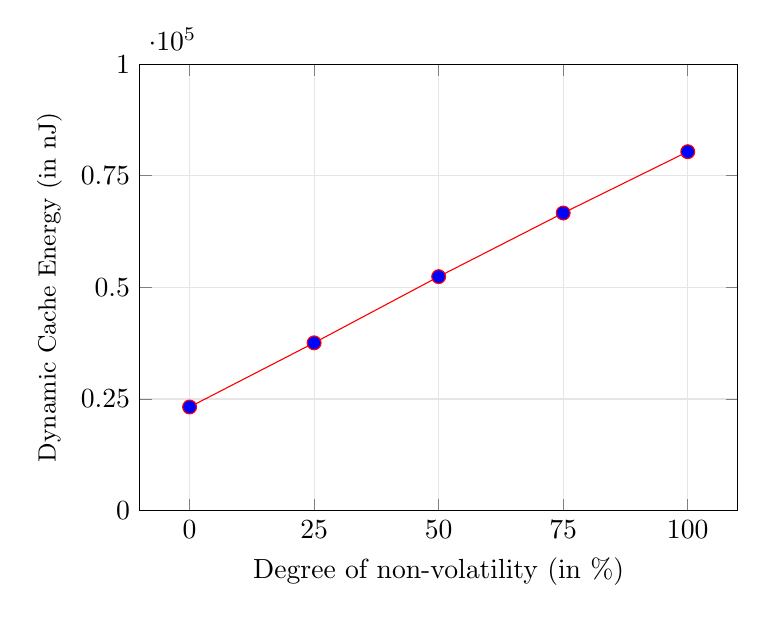
\begin{tikzpicture}
 
\begin{axis}[
	xmin = -10,
	xmax = 110,
	xtick distance = 25,
	ymin = 0,
	ymax = 100000,
	ytick distance = 25000,
    grid = both,
    major grid style = {gray!20},
    width = \columnwidth,
    height = 0.78\textwidth,
    xlabel = { \normalsize Degree of non-volatility (in \%)},
    ylabel = {\small Dynamic Cache Energy (in nJ)},
    scale = 0.72
    ]

\addplot[red,mark=*,mark options={scale=1.25, fill=blue},text mark as node=true,point meta=explicit symbolic] coordinates { (0,23217.578001) (25,37583.014876) (50,52414.414793) (75,66654.849654) (100,80393.959481)};

\end{axis}
\end{tikzpicture}
	\end{subfigure}
    \caption{Latency and dynamic energy consumption under different degrees of non-volatility for a write-intensive merge sort application.}
    \label{fig:FAUmsort}
\end{figure}

\begin{figure}
	\begin{subfigure}{0.475\textwidth}
		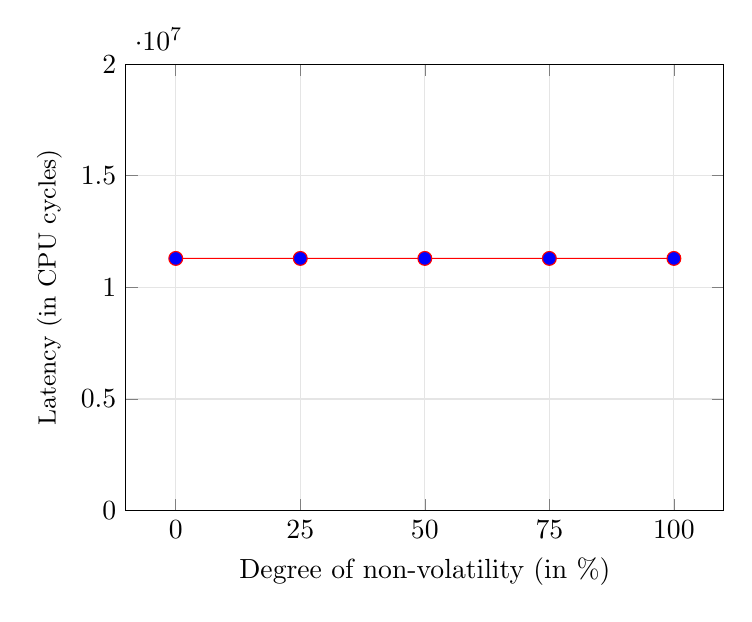
\begin{tikzpicture}
 
\begin{axis}[
	xmin = -10,
	xmax = 110,
	xtick distance = 25,
	ymin = 0,
	ymax = 20000000,
	ytick distance = 5000000,
    grid = both,
    major grid style = {gray!20},
    width = \columnwidth,
    height = 0.78\textwidth,
    xlabel = { \normalsize Degree of non-volatility (in \%)},
    ylabel = {\small Latency (in CPU cycles)},
    scale = 0.72
    ]

\addplot[red,mark=*,mark options={scale=1.25, fill=blue},text mark as node=true,point meta=explicit symbolic] coordinates { (0,11298120) (25,11298143) (50,11298143) (75,11298118) (100,11298118)};

\end{axis}
\end{tikzpicture}
	\end{subfigure}
	\begin{subfigure}{0.475\textwidth}
		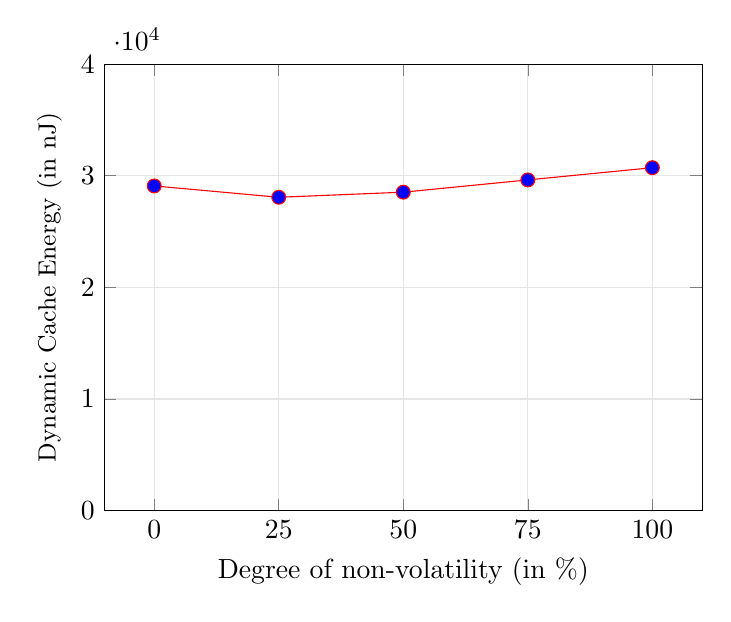
\begin{tikzpicture}
 
\begin{axis}[
	xmin = -10,
	xmax = 110,
	xtick distance = 25,
	ymin = 0,
	ymax = 40000,
	ytick distance = 10000,
    grid = both,
    major grid style = {gray!20},
    width = \columnwidth,
    height = 0.78\textwidth,
    xlabel = { \normalsize Degree of non-volatility (in \%)},
    ylabel = {\small Dynamic Cache Energy (in nJ)},
    scale = 0.72
    ]

\addplot[red,mark=*,mark options={scale=1.25, fill=blue},text mark as node=true,point meta=explicit symbolic] coordinates { (0,29088.925748) (25,28074.614715) (50,28530.362257) (75,29628.430611) (100,30723.784948)};

\end{axis}
\end{tikzpicture}
	\end{subfigure}
    \caption{Latency and dynamic energy consumption under different degrees of non-volatility for a read-intensive image processing application.}
    \label{fig:FAUip}
\end{figure}

\textit{Latency:} We can identify, that a higher degree of non-volatility barely influences the overall latency, despite the high NVM write latency.
This is explained by the fact, that in case of a cache write the CPU does not stall until the write is completed, unless data from the very same cache line is required in the meantime, which is rarely the case.

\textit{Dynamic Energy:} While the observation in the latency dimension holds for both applications, the dynamic energy under varying degrees of non-volatility behaves differently for the two applications.
For the write-intensive merge sort application, displayed in \cref{fig:FAUmsort}, the dynamic energy consumption rises proportionally with the increased degree of non-volatility.
This is to be expected, as the higher degree of non-volatility also implies a higher number of high energy NVM writes.
However, this is not the case for the image processing experiment, as seen in \cref{fig:FAUip}.
Here, as the application is highly read-intensive with read accesses in STT-RAM being more energy efficient than in SRAM, introducing NVM to a low degree can even reduce the dynamic energy consumption of the cache.
Using the toolchain with our hybrid cache extensions, we can thus analyze in which application scenarios and to which degree the introduction of NVM to the cache hierarchy proves the most beneficial.
Furthermore, for this case study, no replacement policies that consider the characteristics of the underlying memory technologies were analyzed.
These policies performing placement decisions according to, e.g., the predicted write intensity of future accesses, can further boost the performance of hybrid caches to a notable degree \cite{8716297,7110550, Wilbert:2024a}.

\subsubsection{Step-by-Step Instructions}
In the following we will provide a step-by-step guide on how hybrid caches are implemented in gem5.
First, we will create a \texttt{HybridCache} \texttt{SimObject} by inheriting the base methods from gem5's base cache class located in \texttt{src/mem/cache/base.cc}.
To account for the hybrid cache's asymmetric read/write latencies, we add additional parameters for the read and write latency of the non-volatile STT-RAM section.
Additionally, in order to generate meaningful statistics that allow for the analysis of hybrid caches, we add statistics for the dynamic energy consumption and number of accesses per section.
The gem5 \texttt{CacheBlk}, representing a cache line, is extended to a \texttt{HybridCacheBlk}, carrying the additional information whether the cache line is considered to be implemented in a volatile or non-volatile manner.
Whenever a cache line is accessed in the extended base cache class, we check for the volatility of the corresponding \texttt{HybridCacheBlk}.
Depending on whether the cache line is volatile or not, we thus take the latency and energy parameters for the SRAM or the STT-RAM section, respectively, as seen in the following listing where we exemplarily display the code for setting the latency and logging statistics following a write access to the hybrid cache.
\begin{lstlisting}[language=C]
HybridCacheBlk* hyblk = dynamic_cast<HybridCacheBlk*>(blk);
Cycles lat = hyblk->isVolatile() ? dataLatency : dataWriteLatency;
if (hyblk->isVolatile()) {
	hybrid_stats.noOfVolWrites++;
	hybrid_stats.dynEnergy += volWriteEnergy;
} else {
	hybrid_stats.noOfNonVolWrites++;
	hybrid_stats.dynEnergy += nonVolWriteEnergy;
}
\end{lstlisting}
The cache lines themselves are initialized and managed in the \texttt{BaseTags} class located in \texttt{src/mem/cache/tags/base.cc}.
To set the cache lines as volatile/non-volatile in accordance to the previously described \texttt{nvBlockRatio} parameter, we set the \texttt{HybridCacheBlk}'s volatile flag in the \texttt{HybridSetAssoc} class, which is derived from the \texttt{BaseTags} class.
\begin{lstlisting}[language=C]
int numNvBlocksPerSet = (nvBlockRatio/100)*assoc;
int numNvBlocksInSet = 0;
// Initialize all blocks
for (int blk_index = 0; blk_index < numBlocks; blk_index++) {
    HybridCacheBlk* blk = &blks[blk_index];
    if (blk_index 
        numNvBlocksInSet = 0;
    // Set whether block is volatile or non-volatile
    if (numNvBlocksInSet < numNvBlocksPerSet) {
        blk->setVolatile(false);
        numNvBlocksInSet++;
    } else {
        blk->setVolatile(true);
    }
}
\end{lstlisting}
On the Python configuration level in \texttt{configs/common/Caches.py}, we can define, e.g., L1 Data Caches as shown below, which are derived from the introduced \texttt{HybridCache} class, with hybrid-cache-specific parameters set to any desired value.
\begin{lstlisting}[language = Python]
class L1DCache(HybridCache):
    assoc = 4
    nv_block_ratio = 50
    data_read_latency = 2
    data_write_latency = 8
    ...
\end{lstlisting}
The connection between the C++ \texttt{SimObjects} containing the functional implementation and the Python classes setting a configuration is realized in \texttt{src/mem/cache/Cache.py} as follows.
\begin{lstlisting}[language = Python]
class HybridCache(ClockedObject):
    type = 'HybridCache'
    cxx_header = 'mem/cache/hybrid_cache.hh'
    cxx_class = 'gem5::HybridCache'
    data_read_latency = Param.Cycles("Data read access latency")
    data_write_latency = Param.Cycles("Data write access latency")
    ...
\end{lstlisting}
Furthermore, the additional hybrid-cache-specific parameters which can be set in the configuration files are named here.
For the \texttt{HybridSetAssoc} class, this is performed analogously in the \texttt{src/mem/cache/tags/Tags.py} file.
By running a gem5 simulation with Cache \texttt{SimObjects} of the \texttt{HybridCache} type, the analysis of heterogeneous cache architectures is thus made possible.
See \cref{app:fau}, for a more detailed description of the concrete command to perform and evaluate a simulation run.
\begin{insightbox}
In this case study, we have learned how gem5 can be extended to support caches incorporating both SRAM and STT-RAM cells.
We have observed in the experiments, that the write latency overhead of STT-RAM is barely noticeable in application scenarios.
While the introduction of NVM inherently lowers static power consumption in caches, even under conventional replacement policies, hybrid caches can further reduce dynamic energy consumption, depending on the characteristics of the application.
Owing to gem5's flexibility, our extension thus provides the opportunity to quickly evaluate the potential of hybrid caches when developing novel cache policies or investigating novel use-cases.

\end{insightbox}

\subsection{Compute-in-Memory (CiM)} \label{sec:nvm-cim}


\subsubsection{Overview}

Modern computing systems predominantly rely on the von Neumann architecture \cite{kit1}, where the CPU handles data processing and memory components are dedicated to storage \cite{kit2}. This design results in frequent data transfers between the CPU and memory, causing significant energy consumption and performance bottlenecks, collectively known as the ``memory wall.'' These transfers account for up to 60\% of system energy use, with memory access consuming far more energy than computational operations \cite{kit3,kit4,kit5}. Additionally, DRAM faces scaling limitations, with its capacity growth lagging behind increases in processing power, partly due to the shrinking reliability of DRAM cells \cite{kit/dramScale1,kit/dramScale2,kit/dramScale3}.

The Compute-in-Memory (CiM) architecture has emerged as a viable solution to reduce the energy cost of data movement. By bringing processing capabilities closer to the data, CiM reduces reliance on the CPU \cite{kit/ext1,kit/ext2,kit/ext3}. These architectures range from minimal hardware changes for simple operations, such as bulk data manipulation, to more complex designs integrating processing cores near memory arrays. While the latter supports a wide range of applications, challenges such as design complexity, frequent CPU interactions, and task-offloading inefficiencies limit their practicality \cite{kit/ext2}. Simplified CiM designs, focusing on specific applications, reduce information exchange with the CPU and ease programming challenges, making them ideal for parallelizable tasks like DNA sequencing \cite{kit/dna1,kit/dna2, hameed_tetc21}, image processing \cite{kit/img1,kit/img2}, and database operations \cite{kit/db1,kit/db2}.
As advanced memory technologies that tightly couple memory with logic units have entered mass production (e.g., HBM \cite{kit/hbm} and HMC \cite{kit/hmc}), CiM is the industry's next frontier~\cite{khan_cimlandscape_2024}.

However, current research has mostly focused on SRAM-based and DRAM-based CiM architectures, leaving a gap in tools for NVM-based CiM design and evaluation. NVMs, as discussed in \cref{sec:Introduction}, offer significant advantages such as reduced static power leakage, no need for data refreshing, and improved scalability. These properties make NVMs particularly promising for CiM, where energy efficiency and scalability are critical \cite{kit/ext1,kit/ext4}. NVM like ReRAM has resistive properties that enable efficient analog-based MAC and Boolean computations with minimal hardware modifications.


Recent advancements in NVM-based CiM modules demonstrate their potential for practical implementations. Leading foundries, including TSMC, Samsung, and IBM, have fabricated CiM modules using ReRAM, STT-MRAM, and PCM. For instance, TSMC has integrated ReRAM and STT-MRAM into CiM designs for neural network acceleration \cite{kit/stt-tsmc1,kit/reram-tsmc4}, while Samsung and IBM have demonstrated CiM modules using STT-MRAM and PCM \cite{kit/pcm-ibm3,kit/stt-samsung2}, respectively. These developments showcase the ability of NVM-based CiM architectures to address the performance and energy limitations of traditional computing systems, highlighting their potential to enable more efficient and scalable designs.



\subsubsection{Objective}

Existing CiM simulators, such as CIM-SIM \cite{CIM-SIM}, MNSIM \cite{MNSIM}, NeuroSiM \cite{NEUROSIM}, PiMulator \cite{PiMulator}, MultiPIM \cite{MultiPIM}, Sim2PIM \cite{Sim2PIM}, and PIMSim \cite{PIMSim}, offer capabilities like full-system simulation, reconfigurable technology and architecture, and cycle-accurate modeling.
However, our CiM extension is the first to integrate all these features specifically for NVM.
Designed with detailed modeling, modularity, and extensibility,
our extension prioritizes realistic design choices to ensure practical applicability in real-world scenarios.
The following subsections provide an in-depth exploration of these features.


\subsubsection{Methodology}

To gain a deeper understanding of the proposed CiM extension, we begin by discussing the general design choices, the available alternatives, and the reasoning behind these decisions. This approach helps readers comprehend the requirements for practical architectural design while enabling them to identify potential improvements and trade-offs. Subsequently, we provide a detailed implementation guide for the gem5 framework in the following subsections.

\textbf{CiM vs. PIM:}
A central distinction in this design is between CiM and PIM (Processing-in-Memory). PIM integrates processing cores near memory to support diverse applications but faces challenges such as complex design, frequent CPU data exchanges, and system support issues (e.g., coherency mechanisms and task-offloading granularity)  \cite{kit/ext1,kit/ext4,kit/ext5,kit/ext7}.
CiM, by contrast, focuses on minimal modifications to the memory periphery for specific tasks like bulk bitwise operations or data copying \cite{kit/rowclone}. This narrower scope simplifies programming, reduces CPU interaction, and enables a streamlined design. Additionally, CiM leverages the unique resistive properties of NVM for efficient analog computations, such as MAC and Boolean operations \cite{kit/ext4,kit/ext5,kit/ext8}, using simple crossbar circuitry modifications. This design resembles SIMD cores with much larger register sizes (equivalent to a memory bank’s row), making CiM highly efficient for parallelized, data-intensive applications.

\textbf{CPU-CiM Communication:}
This can be implemented in two ways:
\CRicon{1} Custom Instructions and \CRicon{2} Memory-Mapped I/O. While the The first approach is well-suited for accelerators closely connected to the CPU core. However, it requires significant CPU modifications (e.g., pipeline and control logic changes) and is tied to specific ISAs, which limits compatibility.
The second approach maps the CiM module’s physical address space into the virtual address space of applications. While it introduces communication delays due to OS involvement, it avoids the design challenges of custom instructions and is more flexible, making it the preferred choice in this case.

\textbf{Physical Placement of CiM Components:}
A critical design decision for CiM components is their physical placement within the main memory module, which consists of multiple memory chips. While integrating CiM circuitry directly into each chip allows for parallel processing of simple operations like logical AND, it faces challenges with operations like logical shifts that require contiguous data. Modeling CiM as a separate chip adjacent to memory chips addresses some issues but introduces power, latency, and communication protocol challenges due to the DDR interface’s lack of dedicated signal lines. Despite these trade-offs, using LRDIMM (Load-Reduced Dual In-Line Memory Module) modules, commonly found in server applications, offers a practical solution. LRDIMMs enhance signal integrity, reduce system modifications, and provide added benefits like error correction and improved simulation flexibility, making them ideal for CiM integration.

Finally, memory controllers, which are highly complex and integrated into modern CPUs, present a unique challenge for CiM implementation. Modifying these controllers requires careful consideration to avoid performance bottlenecks or compatibility issues. Proposals involving such changes must carefully balance hardware and software implications.
As with other extensions discussed in this article, we utilize the gem5 framework \cite{kit/gem5-1,kit/gem5-2} for modeling and simulation purposes.
\cref{kit:fig1a} shows a simplified X86 system where minimal changes are required for CiM integration. Only a few components within the LRDIMM module are modified, while the CPU-integrated memory controller and memory chips remain unchanged.

\begin{figure}[ht]
	\centering
	\begin{minipage}[c]{0.4\textwidth}
		\centering
		\includegraphics[width=\textwidth, page=1]{KIT-figures/mainSys.pdf} 
		\caption{x86 with CiM-capable memory}
		\label{kit:fig1a}
	\end{minipage}
	\hfill
	\begin{minipage}[c]{0.49\textwidth}
		\centering
		\includegraphics[width=\textwidth, page=2]{KIT-figures/mainSys.pdf} 
		\caption{Structure of the CiM chip}
		\label{kit:fig1b}
	\end{minipage}
\end{figure}


\subsubsection{Step-by-Step Instructions}\label{kit/label1}

This subsection discusses the programming model for the CiM extension, provides examples and supported operations, and concludes with a brief discussion on how it is enabled in gem5. The CiM extension operates similarly to a SIMD core, with CiM rows acting as registers and supporting only simple operations on column-aligned data. A CiM-capable chip resembles a conventional memory chip with modifications to row decoders (`\texttt{Dec.}', for multi-row activation) and sense amplifiers (`\texttt{SA}', for multi-reference voltages), as illustrated in \cref{kit:fig1b}. Simple operations, like bitwise AND, are performed by simultaneously activating rows and applying the appropriate reference voltage across the sense amplifiers.
To support more complex operations, CMOS-based CiM Logic is added after the column selector multiplexer, enabling tasks like bitwise NOT. Input signals for these units are managed by a state machine in the CiM controller, which processes commands from user applications. As illustrated in \cref{kit/fig2}, a NAND operation involves activating operand rows for a parallel AND (step \CRicon{1}), loading results into the CiM Logic for a NOT operation (steps \CRicon{2} to \CRicon{3}), and storing the final results back into memory (step \CRicon{4}). \cref{kit/lst1} shows the implementation of the NAND operation in a user application with the help of CiM API.
To provide a practical example that includes both a loop and a conditional statement, \cref{kit/lst2} presents a sequential \texttt{for} loop in regular C++ code that uses the ternary operator (`\texttt{?:}'), and \cref{kit/lst3} shows the conversion of this code into the CiM version, with the loop unrolled.

\begin{figure}[h]
	\centering
	\includegraphics[width=0.195\linewidth, page=1]{KIT-figures/steps.pdf}
	\includegraphics[width=0.195\linewidth, page=2]{KIT-figures/steps.pdf}
	\includegraphics[width=0.195\linewidth, page=3]{KIT-figures/steps.pdf}
	\includegraphics[width=0.195\linewidth, page=4]{KIT-figures/steps.pdf}
	\includegraphics[width=0.195\linewidth, page=5]{KIT-figures/steps.pdf}
	\caption{Steps required to perform a NAND operation.}
	\label{kit/fig2}
\end{figure}


\cref{kit-tb1} lists the essential operations implemented in the CiM extension. We have applied these operations to several real-world applications, including the following:
\CRicon{1} BitIndexing (BIT)\cite{kit/app1}: Bitmap-formatted database queries are ORed together, and the results are ANDed with another query.
\CRicon{2} BLASTN algorithm (BLS)\cite{kit/app2}: Used for searching short DNA sequences within large DNA or protein sequences.
\CRicon{3} Morphological Image Processing (MIP)\cite{kit/app3}: Implementation of Dilation and Erosion algorithms with binary-coded input images of various filter sizes.
\CRicon{4} Marching Squares (MSQ)\cite{kit/app4}: An algorithm designed to extract contour lines from 2D images.
\CRicon{5} Shifted Hamming Distance (SHD)\cite{kit/app5}: A well-known algorithm for calculating edit distances in short DNA sequences.
\CRicon{6} BitWeaving (BWV)\cite{kit/app6}: A technique developed for efficiently scanning database queries in memory.
These applications are categorized as \textit{Embarrassingly Parallel} \cite{kit/emb}, making them well-suited for CiM implementation.
Other operations, such as MAC for binarized vector-to-matrix multiplication, are also included in the source files to support the implementation of simple neural network applications.
Users can refer to the provided application examples, CiM API code and documentation, as well as other modules, such as OS drivers offered by the CiM API, to gain a better understanding of CiM implementation.


\begin{table}[h]
	\caption{Essential operations supported by the CiM extension.}
	\label{kit-tb1}
	\begin{tabular}{@{}ccccc@{}}
		\toprule
		Operation Type                                                                                     &
		Operation                                                                                          &
		Source                                                                                             &
		Destination                                                                                        &
		Description                                                                                                                               \\ \midrule
		In Memory Array                                                                                    &
		\texttt{AND, OR, XOR}                                                                              &
		A List of Rows                                                                                     &
		\begin{tabular}[c]{@{}c@{}}A Single Row\\ (Default: \texttt{SA} output)\end{tabular}                        &
		Perform bitwise operation                                                                                                             \\ \midrule
		\multirow{2}{*}[-6pt]{In CMOS Periphery}                                                           &
		\texttt{COPY}                                                                                      &
		\multirow{2}{*}[-6pt]{\begin{tabular}[c]{@{}c@{}}A Single Row\\ (Default: \texttt{SA} output)\end{tabular}} &
		\multirow{2}{*}[-6pt]{A Single Row}                                                                &
		\begin{tabular}[c]{@{}c@{}}Copies row content\\ Optional: bitwise rotation\end{tabular}                                               \\ \cmidrule(lr){2-2} \cmidrule(l){5-5}
		                                                                                                   &
		\texttt{NOT\_COND}                                                                                 &
		                                                                                                   &
		                                                                                                   &
		\begin{tabular}[c]{@{}c@{}}Performs bitwise NOT\\ Or vector mask operation.\end{tabular}                                              \\ \midrule
		\multirow{2}{*}[-3pt]{\begin{tabular}[c]{@{}c@{}}In CiM Controller\\ Or DMA-Related\end{tabular}}        &
		\texttt{copy\_to\_cim}                                                                             &
		A pointer to a vector                                                                              &
		CiM row number                                                                                     &
		\multirow{2}{*}[-3pt]{\begin{tabular}[c]{@{}c@{}}Copies vector to/from a CiM row\\ If DMA:  Main Memory $\leftrightarrow$ CiM\end{tabular}} \\ \cmidrule(lr){3-4}
		                                                                                                   &
		\texttt{copy\_to\_cpu}                                                                             &
		CiM row number                                                                                     &
		A pointer to a vector                                                                              &
		\\ \bottomrule
	\end{tabular}
\end{table}

To summarize, \cref{kit/fig3} illustrates the modifications made to the gem5 framework to enable the CiM extension. The only alterations to the gem5 codebase involve the \texttt{AbstractMemory} class, which has been adapted to monitor interactions with the CiM address space, and the \texttt{MemInterface} class, which has been updated to adjust the access time for any request associated with the CiM address space. The \texttt{CiMHandler} class serves as the primary component responsible for managing CiM commands. It accomplishes this by interpreting opcodes, configuring the state machine, assigning appropriate timing, and ultimately invoking the relevant operation function via the \texttt{CiMOperationInterface}.
The \texttt{CiMOperationInterface} acts as the base class for all CiM operations, providing a pure functional implementation. This class can be extended to incorporate detailed modeling or fault injection capabilities (e.g., the \texttt{CiMFaultInjection} class, as shown). Most parameters can be configured through the gem5 simulation configuration file, allowing users to select among different technologies or specify various timing values. Additionally, users can extend the source code by overriding the provided functions.
Finally, as with the previous extensions discussed in this article, either the `\texttt{CDNCcim=1}' or `\texttt{CDNCcimFS=1}' flag must be specified during the gem5 compilation process, depending on the desired simulation mode (system emulation/full-system simulation mode), to enable the CiM extension.
Detailed steps for setting up and running the CiM extension are provided in the Appendices section.


\begin{figure}[h]
	\centering
	\includegraphics[width=0.8\linewidth, page=3]{KIT-figures/mainSys.pdf}
	\caption{Summary of modifications, contributions, and communications regarding the CiM extension in gem5.}
	\label{kit/fig3}
\end{figure}

\begin{insightbox}
	This case study provides a comprehensive guide to the practical realization of CiM, highlighting key challenges and offering researchers clear directions for getting started.
	Our CiM extension stands out by combining full-system simulation, flexible technology and architecture, and detailed circuit modeling, specifically targeting NVM technologies.
	It focuses on accuracy, reconfigurability, and expandability, enabling realistic design decisions and facilitating hardware/software design-space exploration for CiM applications.
\end{insightbox}


\section{Conclusion}
In this collaborative work from the SPP 2377 priority program, we present a tutorial that demonstrates extensions to a toolchain based on gem5 and NVMain. We show how to use the toolchain for architectural exploration and development of co-design strategies for emerging memory technologies. Four case studies were discussed: hybrid main memory, trace-based wear-out analysis, heterogeneous cache design, and compute-in-memory architectures. These case studies not only demonstrate the toolchain's versatility and depth, but also provide researchers with the knowledge they need to extend and customize it for their specific applications. We also provide open access to the source code and setup instructions in the hope of increasing the reproducibility of research in NVM co-design.

\bibliographystyle{plain}
\bibliography{references}


\section{Notação do Espaço  $\ell _{p}$ das Normas}\label{Ap:normas1}

 A norma é uma função que mapeia números reais ou complexos para números não-negativos e apresenta as propriedades da desigualdade triangular, da homogeneidade absoluta e de ser positiva definida \cite[pág. 68-9]{golub2013matrix}. Quando a última propriedade tal não é respeitada, ou seja, que o resultado possa ser nulo, mesmo com o argumento não-nulo, ela é chamada de seminorma. 

No caso de vetores, seja $p \geq  1$ um número real, $n$ o número de elementos do vetor e $1\leq i \leq n$. A norma $\ell _{p}$ de um vetor $\mathbf{x} =(x_{1},\ldots ,x_{n})$ de números reais é definida por \cite[pág. 69]{golub2013matrix}
\begin{equation}
\begin{aligned}
| | \mathbf{x} ||_{p} & =   \left(\sum _{i=1}^{n}\left | x_{i}\right|^{p}\right)^{1/p}    \\
& =  \left(| x_{1}|^{p}+| x_{2}|^{p}+\dots +| x_{n}|^{p}\right)^{1/p},     
\end{aligned}
\label{eq:lpnorm}
  \end{equation}
  onde $\vert x_i\vert$ é o valor absoluto, ou módulo, do i-ésimo valor de $\mathbf{x}$.  
  
  Nesse caso, a norma pode ser entendida como uma medida de distância em relação à origem. Caso o argumento da norma seja uma diferença entre vetores $| | \mathbf{x} - \mathbf{y} ||_{p}$, a norma representa a distância entre eles. 
  
Seja também o caso em que a Equação \eqref{eq:lpnorm} é elevada à potência $p$, isto é, 
\begin{equation}
\vert \vert \mathbf{x} \vert\vert_{p}^p =    \vert x_{1}\vert^{p}+\vert x_{2}\vert^{p}+\dotsb +\vert x_{n}\vert^{p}.
\label{eq:lpnormp}
  \end{equation}
Partindo das Equações \eqref{eq:lpnorm} e \eqref{eq:lpnormp}, são destacados alguns casos específicos:
\begin{itemize}
 \item Para $p = 1$, tem-se a distância absoluta:
\begin{equation}
\begin{aligned}
\vert \vert \mathbf{x} \vert\vert_{1} & =   \left(\vert{x_{1}\vert}^{1}+{\vert x_{2}\vert}^{1}+\dotsb +{\vert x_{n}\vert}^{1}\right)^{1/1}  \\
     & =    \vert x_{1}\vert + \vert x_{2}\vert + \dotsb +\vert x_{n}\vert.
\end{aligned}
 \end{equation}
 Observa-se que $\vert \vert \mathbf{x} \vert\vert_{1} = \vert \vert \mathbf{x} \vert\vert_{1}^1$, onde o expoente $1$ é usualmente omitido.
 
    \item Para $p = 2$, tem-se a norma euclidiana:
  \begin{equation}
  \begin{aligned} 
\vert \vert \mathbf{x} \vert\vert_{2}& =  \left(\vert x_{1}\vert^{2}+\vert x_{2}\vert^{2}+\dotsb +\vert x_{n}\vert^{2}\right)^{1/2} \\       
& =  \left({x_{1}}^{2}+{x_{2}}^{2}+\dotsb +{x_{n}}^{2}\right)^{1/2}.
    \end{aligned}
\end{equation}
Outras representações e notações são obtidas com o produto interno conforme $\vert \vert \mathbf{x} \vert\vert_{2} = \sqrt{\langle \mathbf{x}, \mathbf{x} \rangle} = \sqrt{\mathbf{x} \cdot \mathbf{x}} = \sqrt{\mathbf{x}^T \mathbf{x}}$. 
 \item O quadrado da norma euclidiana é dado por:
\begin{equation}
\begin{aligned}
\vert \vert \mathbf{x} \vert\vert_{2}^2 & =   \mathbf{x}^T \mathbf{x} \\
& =   {x_{1}}^{2}+{x_{2}}^{2}+\dotsb +{x_{n}}^{2}.
\end{aligned}
\end{equation}
 
 \item O quadrado da norma euclidiana ponderada \cite[pág. 666]{Sayed2003} pode ser denotado:
\begin{equation}
\begin{aligned}
\vert \vert \mathbf{x} \vert\vert_{W}^2  & =   \mathbf{x}^T \mathbf{W} \mathbf{x} \\
 & = \vert \vert \mathbf{W}^{\frac{1}{2}} \mathbf{x} \vert\vert_{2}^2.
\label{eq:weighted}
\end{aligned}
\end{equation}
\item Para $p = \infty$, tem-se a chamada norma infinito, também conhecida como norma do supremo ou norma uniforme, que retorna a maior magnitude entre os elementos de um vetor. Matematicamente isso é representado por 
\begin{equation}
\vert \vert \mathbf{x} \vert\vert_{\infty }=\max \left\{\vert x_{1}\vert,\vert x_{2}\vert,\dotsc ,\vert x_{n}\vert\right\}.  
\end{equation}
\item Para $0 < p<1$, a propriedade da desigualdade triangular não é respeitada, de modo que neste caso não se tem uma norma propriamente dita. Para fins de visualização também será utilizada a Equação \eqref{eq:lpnorm}.
\item Para $p=0$, também não se tem uma norma pela definição, mas há autores que entendem $\vert \vert \mathbf{x} \vert\vert_{0}$ como a contagem de números não-nulos de $\mathbf{x}$ \cite{Donoho2006}.
\end{itemize}

\subsection{Visualização de diferentes normas $\ell_p$}
Seja o vetor com dois elementos $\mathbf{x} = (x_1, x_2)$ e seja $|| \mathbf{x} ||_{p} = 1$. Na Figura \ref{fig:my_labelaaa} são mostrados os gráficos da Equação \eqref{eq:lpnorm} para diferentes valores de $p$. 

\begin{figure}[H]
    \centering
    \includegraphics[width = 0.65\linewidth]{figures/modulo2.png}
    \caption[Normas visualizadas no círculo unitário.]{Normas visualizadas no círculo unitário. Fonte: Próprio Autor. }
    \label{fig:my_labelaaa}
   
\end{figure}
Valores de $p<1$ não definem uma norma, mas é importante a visualização da sua não-convexidade.  Extrapolando essa ideia, a norma para $p = 0$ estaria nos próprios eixos coordenados, que foram omitidos para melhor visualização dos demais gráficos. O outro caso limite é norma infinito, que nessa mesma figura é o quadrado com centro em (0,0) e lado de tamanho = 2, em volta dos demais gráficos. 

\subsubsection{Comparação entre as normas $\ell_2$, $\ell_1$ e $\ell_0$ }
A Figura \ref{fig:01_021} mostra duas visualizações\footnote{Provenientes do conceito de \textit{ball} \cite[Capítulo 2]{Gopal2020}, nesse caso uma \textit{ball} unitária com norma $\ell_p$.} semelhantes \cite[Subseção 2.10]{Gopal2020}. Elas são importantes para explicar a promoção da esparsidade, bem como utilizada para ilustrar a equivalência entre soluções de normas $\ell_1$ e $\ell_0$, pois, sob certas condições, a norma $\ell_0$ poderia resultar na mesma solução que a norma $\ell_1$ \cite[págs. 30-1]{majumdar2019compressed}. 

Na Figura \ref{fig:01_021a}, baseada em \cite[Figura 2.21]{Gopal2020}:
\begin{itemize}
\item A circunferência azul-escuro é obtida a partir de uma equação de norma $\ell_2$, $\vert \vert \mathbf{x} \vert \vert_2 = 1$ e o quadrado vermelho é obtido a partir de uma equação de norma $\ell_1$, $\vert \vert \mathbf{x} \vert \vert_1 = 1$;
\item Uma solução da minimização da norma $\ell_2$ restringida pela reta amarela $\mathbf{A} \mathbf{x}_1 = \mathbf{y}$ é o ponto onde a reta e a circunferência se tangenciam, com $\mathbf{x}$ e $\mathbf{y}$ não-nulos;
\item Uma solução da minimização da norma $\ell_1$ restringida pela reta roxa $\mathbf{A} \mathbf{x}_2 = \mathbf{y}$ também é o ponto onde elas se interceptam, agora no eixo $\mathbf{y}$, onde um parâmetro é nulo e um é não-nulo, uma solução mais esparsa do que $\mathbf{x}_1$ obtida com a norma $\ell_2$.
\end{itemize}

Na Figura \ref{fig:01_021b}, baseada em \cite[pág. 182]{aster2019parameter}, a ideia é a mesma, mas a norma do quadrado deixa de ser unitária para que a solução esteja contida na mesma reta azul, tangenciando tanto a circunferência quanto o quadrado simultaneamente.
\begin{figure}[H]
     \centering
     \begin{subfigure}[b]{0.45\textwidth}
         \centering
         \includegraphics[width=\textwidth]{figures/lp12.png}
         \caption{a) Primeira visualização}
         \label{fig:01_021a}
     \end{subfigure}
     \hfill
     \begin{subfigure}[b]{0.45\textwidth}
         \centering
         \includegraphics[width=\textwidth]{figures/lp22.png}
         \caption{b) Segunda visualização}
         \label{fig:01_021b}
     \end{subfigure}
         \caption[Duas visualizações para soluções com normas $\ell_1$ e $\ell_2$.]{Duas visualizações para soluções com normas $\ell_1$ e $\ell_2$. Fonte: Próprio autor.}
        \label{fig:01_021}
\end{figure}



\newpage
\section{Matrizes pseudoinversas} \label{Ap:sobredet}

Neste apêndice, são desenvolvidos os conceitos apresentados na Subseção \ref{sec:excess}. 

\subsection{Sistema sobredeterminado}
Seja um sistema linear de equações do tipo $\mathbf{A}\mathbf{x} = \mathbf{y}$.  Se a matriz $\mathbf{A}$ possuir mais equações do que variáveis (mais linhas do que colunas), um sistema sobredeterminado, não há solução exata e só é possível obter uma solução aproximada. Pode-se buscar, por exemplo, a solução que minimize a soma do quadrado entre os termos da esquerda e da direita do sistema linear \cite[pág. 29]{matrixcookbook}, conforme
\begin{equation}
\hat{\mathbf{x}} = \arg\min\limits_{\mathbf{x}} \left( \vert \vert \mathbf{A}\mathbf{x} - \mathbf{y} \vert \vert^2_2 \right).
    \label{eq:otimizacao12} 
\end{equation}
Pode-se reescrever a expressão anterior como
\begin{equation}
\begin{aligned}
    \vert \vert  \mathbf{A}\mathbf{x} - \mathbf{y}\vert \vert^2_2 & = \left( \mathbf{A}\mathbf{x} - \mathbf{y}\right)^T \left( \mathbf{A}\mathbf{x} - \mathbf{y}\right) \\
    & = \mathbf{y}^T\mathbf{y} - \mathbf{y}^T \mathbf{A}\mathbf{x} - \mathbf{x}^T \mathbf{A}^T \mathbf{y} + \mathbf{x}^T \mathbf{A}^T \mathbf{A} \mathbf{x},
    \label{eq:funcional_app}
      \end{aligned}
\end{equation}
de modo que o seu gradiente em relação a $\mathbf{x}$ é obtido conforme
\begin{equation}
\nabla_\mathbf{x} \left(\vert \vert  \mathbf{A}\mathbf{x} - \mathbf{y}\vert \vert^2_2\right) = - 2 \mathbf{A}^T\mathbf{y} + 2 \mathbf{A}^T \mathbf{A} \mathbf{x}.
    \label{eq:funcional_app2}
\end{equation}
Pela condição de otimalidade de primeira ordem \cite[Equação 4]{Gerth2021}, iguala-se a zero o gradiente em relação a $\mathbf{x}$, obtido na Equação \eqref{eq:funcional_app2}, de acordo com
\begin{equation}
\nabla_\mathbf{x} \left(\vert \vert  \mathbf{A}\mathbf{x} - \mathbf{y}\vert \vert^2_2\right) = \mathbf{0}.
    \label{eq:funcional_app2-2}
\end{equation}
 Em seguida, rearranjando os termos e multiplicando os dois lados por $\frac{1}{2}$ obtém-se
\begin{equation}
\mathbf{A}^T \mathbf{A}\mathbf{x} = \mathbf{A}^T \mathbf{y}.
\end{equation}
Logo, a solução para este problema é dada por
\begin{equation}
\hat{\mathbf{x}}   = \left(\mathbf{A}^T \mathbf{A} \right)^{-1} \mathbf{A}^T \mathbf{y}.
    \label{eq:normalequation_app}
\end{equation}
Em alguns trabalhos como \cite{hansen2010discrete}, a Equação \eqref{eq:otimizacao12} é apresentada apenas com a norma $\ell_2$, sem estar elevada ao quadrado, conforme
\begin{equation}
\vert \vert \mathbf{A}\mathbf{x} - \mathbf{y} \vert \vert_2 = \sqrt{ \sum_{i=1}^m  \vert\left(A x\right)_i - y_i \vert^2 }, 
\label{eq:normalequation67}
\end{equation}
onde $i$ indica a linha do vetor. 

Usualmente evita-se a raiz quadrada para resolver o problema computacionalmente mais simples. Apesar disso, o mínimo obtido pela otimização não se altera, pois a raiz quadrada é uma função monótona crescente.


\subsection{Sistema subdeterminado}\label{subdet} 
Seja o sistema $\mathbf{A}\mathbf{x} = \mathbf{y}$. Se a matriz $\mathbf{A}$ possui mais variáveis do que equações (mais colunas no que linhas), um sistema subdeterminado, e há infinitas soluções. Isso significa que muitas escolhas possíveis para $\mathbf{x}$ podem resultar no mesmo $\mathbf{y}$. Neste caso, uma opção é restringir as soluções cuja norma do vetor $\mathbf{x}$ seja mínima \cite[pág. 29]{matrixcookbook}, conforme
\begin{equation}
\hat{\mathbf{x}} = \underset{\mathbf{x}}{\arg\min}\vert \vert \mathbf{x} \vert \vert_2^2 \quad \text{s.t.} \quad \mathbf{A}\mathbf{x} = \mathbf{y}.
   \label{casosub_sol_app}
\end{equation}
Pode-se transformar este problema de otimização com restrições em um problema de otimização sem restrições utilizando o método dos multiplicadores de Lagrange. Seja
\begin{equation}
\mathcal{M}(\mathbf{x},\lambda) =   \vert \vert \mathbf{x} \vert \vert^2_2  + \lambda \left(\mathbf{y} - \mathbf{A}\mathbf{x} \right).
\end{equation}
A primeira condição de otimalidade é $\nabla_\mathbf{x}  \mathcal{M}(\mathbf{x},\lambda)  = 0$, de modo que
\begin{equation}
\begin{aligned}
\mathbf{0} & =  2\mathbf{x} + \mathbf{A}^T\lambda  \\
 \mathbf{x} & =  -\mathbf{A}^T \frac{\lambda }{2}.
   \label{eq:x}
 \end{aligned}
\end{equation}  
A segunda condição de otimalidade é $ \nabla_{\lambda}  \mathcal{M}(\mathbf{x},\lambda)  = 0$, resultando em
\begin{equation}
   \mathbf{A}\mathbf{x} - \mathbf{y} = \mathbf{0}.
\end{equation}
Substituindo $\mathbf{x}$ obtido na Equação \eqref{eq:x}, obtém-se
\begin{equation}
\begin{aligned}
  \mathbf{0}& =    \mathbf{A}\left( -\mathbf{A}^T  \frac{\lambda }{2}\right) - \mathbf{y}  \\
 \mathbf{y} & =         -\frac{\lambda }{2} \mathbf{A} \mathbf{A}^T  \\   
    \lambda & = -2(\mathbf{A} \mathbf{A}^T)^{-1} \mathbf{y}.   
        \end{aligned}
\end{equation}
Substituindo $\lambda$ de volta na Equação \eqref{eq:x}, a solução é obtida conforme
\begin{equation}
\hat{\mathbf{x}} = \mathbf{A}^T \left(\mathbf{A} \mathbf{A}^T\right)^{-1} \mathbf{y}.
    \label{normalequation4}
\end{equation}

\subsection{Interpolação com matriz pseudoinversa}\label{Ap:pseudo}

Suponha uma função $y(t) = cos(t) + cos(3t) + \delta$ para $\pi < t < 3\pi$ e $\delta  \sim \mathcal{N}(0, 0.1)$. A partir de medidas discretas $\mathbf{y}$ busca-se uma representação desse sinal em uma base de polinômios dada pela matriz $\mathbf{A}_1$ cujo vetor de parâmetros é $\mathbf{x}_1$, conforme Figura \ref{fig:02_100}.

\begin{figure}[H]
\centering
	    \includegraphics[width=0.75\textwidth]{figures/newmatrix.pdf}
\caption[Sistema de equações da interpolação com polinômios.]{Sistema de equações da interpolação com polinômios. Fonte: Próprio autor.}
\label{fig:02_100}
\end{figure}
Cada coluna da matriz $\mathbf{A}_1$ representa a ordem de um polinômio. Para $n= 10$, do grau zero até o polinômio de 9º grau. Ao invés de calcular seus valores no intervalo original, eles foram calculados em torno de zero, no intervalo $-1.7 < t < 1.7$, para evitar valores muito grandes. As primeiras colunas são mostradas na Figura \ref{fig:02_101}.

As colunas da matriz $\mathbf{A}_1$ são independentes, sendo possível realizar a interpolação como um problema de mínimos quadrados conforme Equação \eqref{eq:normalequation}. A saída $\mathbf{y}_{\mathbf{A}1} =  \mathbf{A}_1 \mathbf{x}_1$ é mostrada na Figura \ref{fig:02_102}. A aproximação acompanha a forma geral da curva original, mas não totalmente os pontos onde as direções mudam.  


\begin{figure}[H]
\centering

\begin{subfigure}[b]{0.49\textwidth}
\centering
	    \includegraphics[width=1\textwidth]{figures/interp1a.png}
\caption{Colunas de $\mathbf{A}_1$.}
\label{fig:02_101}
  \end{subfigure}  
\begin{subfigure}[b]{0.49\textwidth}
\centering
	    \includegraphics[width=1\textwidth]{figures/interp1b.png}
\caption{Resultado.}
\label{fig:02_102}
      \end{subfigure}  
\caption[Interpolação com polinômios.]{Interpolação com polinômios. Fonte: Próprio autor.}
\label{fig:02_10}
\end{figure}


Na sequência, o mesmo procedimento é realizado, mas através de uma matriz $\mathbf{A}_2$ cujas colunas são dadas por $cos(t)$, $cos(2t)$, $cos(3t)$, $sin(t)$, $sin(2t)$ e $sin(3t)$, ou seja, incluem a resposta certa. Na Figura \ref{fig:02_1088} há o esquema de interpolação e na Figura \ref{fig:02_111} há a visualização das três primeiras colunas dessa matriz. Dessa vez, os valores de suas colunas foram calculados no intervalo $-\pi < t < \pi$, que não é exatamente o mesmo, apesar de também ter comprimento de $2\pi$ como o sinal original.


\begin{figure}[H]
\centering
	    \includegraphics[width=0.75\textwidth]{figures/newmatrix2.pdf}
\caption[Sistema de equações da interpolação com senóides.]{Sistema de equações da interpolação com senóides. Fonte: Próprio autor.}
\label{fig:02_1088}
\end{figure}


Calculando-se os parâmetros a partir da Equação 
\begin{equation}
\mathbf{x}_2 = \left(\mathbf{A}_2^T \mathbf{A}_2 \right)^{-1} \mathbf{A}_2^T\mathbf{y},
\end{equation}
o resultado $\mathbf{y}_{\mathbf{A}2} =  \mathbf{A}_2 \mathbf{x}_2$ é mostrado na Figura \ref{fig:02_112}, indicando que essa é uma base melhor de representação para o sinal do que a de polinômios. Agora, o resultado é o esperado. 

\begin{figure}[H]
\centering

\begin{subfigure}[b]{0.49\textwidth}
\centering
	    \includegraphics[width=1\textwidth]{figures/interp1c.png}
\caption{Colunas de $\mathbf{A}_2$.}
\label{fig:02_111}
  \end{subfigure}  
\begin{subfigure}[b]{0.49\textwidth}
\centering
	    \includegraphics[width=1\textwidth]{figures/interp1d.png}
\caption{Resultado.}
\label{fig:02_112}
      \end{subfigure}  
\caption[Interpolação com senos e cossenos.]{Interpolação com senos e cossenos. Fonte: Próprio autor.}
\label{fig:02_11}
\end{figure}

Esse exemplo ilustra a importância do operador direto como uma base de representação. Quanto mais correto ele estiver, melhor será a representação do sinal. 


\newpage
\section{Inversão bayesiana}\label{Ap:estimador}

O método de regularização de Tikhonov traz soluções determinísticas, trazendo uma estimativa razoável das grandezas de interesse a partir dos dados disponíveis \cite[pág. 2]{kaipio2005statistical}. Em seu livro, Tikhonov já utilizava a norma quadrática como regularizador \cite[págs. 72-3]{tikhonov1977solutions}. Em certas aplicações, a busca por soluções suaves é esperada, mas outras informações disponíveis sobre a solução podem existir. 

Nesse contexto, a teoria de inversão estatística é relevante, pois também busca resolver problemas mal-postos, mas agora como um problema de inferência bayesiana, que exige uma densidade de probabilidade \textit{a priori} sobre a incógnita para eliminar modelos que não fazem sentido, mesmo que eles se ajustem aos dados. 

Essa informação \textit{a priori}\footnote{Vale notar que Tikhonov usava a expressão \textit{informações suplementares} \cite[págs. 9, 148]{tikhonov1977solutions} no contexto de regularização, ou mesmo usava a expressão informação \textit{a priori} quando se considerava as incógnitas e os ruídos como processos estocásticos \cite[pág. 149]{tikhonov1977solutions}, mas sem um \textit{framework} bayesiano.}, também conhecido como \textit{prior}, se refere às informações disponíveis que indiquem como a grandeza de interesse deve ser, mas antes do processo de medição. Isto é, o \textit{prior} deve ser independente dos dados $\mathbf{y}$ observados que serão utilizados na reconstrução \cite[Subseção 3.2]{calvetti2007introduction}, \cite[pág. 5]{Calvetti2018a}, \cite[págs. 51, 113]{kaipio2005statistical}. 

 Entre os \textit{priors} possíveis nesse \textit{framework}, estão aqueles que não são facilmente expressadas em termos quantitativos \cite{Calvetti2018a}, como os atlas anatômicos \cite{Moura2021}. Logo, a abordagem bayesiana também traz novas formas de incorporação de informação \textit{a priori} à solução do problema inverso. Conforme será visto, a escolha do \textit{prior} pode ser relacionado com o regularizador da solução de Tikhonov em uma solução determinística.

A inversão bayesiana também parte de um modelo $\mathbf{A}$ que relaciona os seus parâmetros $\mathbf{x}$ com dados $\mathbf{y}$ que apresentam ruídos $\bm{\delta}$, mas $\mathbf{x}$, $\mathbf{y}$ e $\bm{\delta}$ são considerados realizações de variáveis aleatórias. Modelar o problema considerando $\mathbf{A}$ conhecido significa partir da hipótese da validade do operador direto, mas também é possível incluir incertezas no modelo \cite[pág. 13]{Calvetti2018a}. Em resumo, \cite[pág. 52]{kaipio2005statistical}:
\begin{itemize}
\item Inicia-se pela definição de um modelo de ruído, na forma de uma densidade de probabilidade $\pi_E$. Assumindo que a informação disponível sobre $\mathbf{x}$ antes das medições também pode ser codificada em uma densidade de probabilidade, obtém-se a densidade \textit{a priori}  $\pi_{priori}(\mathbf{x})$; 
\item Definidos o modelo de ruído e o \textit{prior}, as observações $\mathbf{y}$ são relacionadas com as incógnitas $\mathbf{x}$ através de uma função de probabilidade condicional;
\item Por fim, são desenvolvidos estimadores para obter a densidade de probabilidade \textit{a posteriori} $\pi_{post}$. 
\end{itemize}

Nas próximas seções, cada uma dessas etapas será aprofundada. 

\subsection{Modelo de ruído}
Seja uma variável aleatória $Y$ observada através de um processo de medição, onde uma realização $Y = \mathbf{y}$ denotam os dados obtidos. A segunda variável aleatória $X$ é a incógnita que não pode ser observada diretamente, onde uma realização é descrita por $X = \mathbf{x}$. Há ainda um ruído aditivo $E$, da qual $E = \bm{\delta}$ é uma realização da variável aleatória, sendo $X$ e $E$ independentes entre si \cite[pág. 56]{kaipio2005statistical}. Supondo uma relação linear entre $X$ e $Y$, o modelo estocástico resultante é dado por
\begin{equation}
Y = \mathbf{A}X + E, 
\label{eq:esti1}
\end{equation}
onde $\mathbf{A}$ é o operador direto. Isolando-se $E$ na Equação \eqref{eq:esti1}, obtém-se o modelo de ruído
\begin{equation}
E = Y - \mathbf{A}X.
\label{eq:esti2}
\end{equation}
É possível, por exemplo, atribuir uma distribuição gaussiana para a variável aleatória $E$, com média $\mu = 0$, variância $s^2_{\bm{\delta}}$ e covariância $s^2_{\bm{\delta}} \mathbf{I}$ \cite[Exemplos 2 e 5]{kaipio2005statistical}, distribuição que pode ser denotada por $E \sim \mathcal{N}(0,s^2_{\bm{\delta}}\mathbf{I})$.

Para uma única realização de cada variável aleatória, a Equação \ref{eq:esti2} se torna
\begin{equation}
\bm{\delta} = \mathbf{y} - \mathbf{A}\mathbf{x}.
\label{eq:estix}
\end{equation}
 Considerando que as variáveis aleatórias sejam absolutamente contínuas, as suas distribuições de probabilidade podem ser expressas em termos das suas densidades de probabilidade \cite[pág. 50]{kaipio2005statistical}. Associando ao ruído uma densidade de probabilidade $\pi_E(\bm{\delta})$ gaussiana, obtém-se
\begin{equation}
\pi_E(\bm{\delta}) \propto \exp\left( -\frac{1}{2 s^2_{\bm{\delta}} } \vert \vert \bm{\delta}\vert\vert^2 \right).
\label{eq:esti4}
\end{equation}

\subsection{Obtenção da densidade de probabilidade condicional}

Definido o modelo de ruído, é possível obter a densidade de probabilidade condicional. Fixando-se em uma realização $X = \mathbf{x}$, o único fator aleatório em $Y$ é dado por E \cite[pág. 42]{calvetti2007introduction}, \cite[pág. 5]{Calvetti2018a}, \cite[pág. 56]{kaipio2005statistical},  e a densidade condicional de probabilidade se torna
\begin{equation}
\pi_{Y|X}(\mathbf{y}|\mathbf{x}) = \pi_E(\bm{\delta}).
\label{eq:esti5}
\end{equation}
Unindo-se a Equação \eqref{eq:esti4} com a Equação \eqref{eq:esti5} obtém-se
\begin{equation}
\pi_{Y|X}(\mathbf{y}|\mathbf{x}) \propto \exp\left( -\frac{1}{2 s^2_{\bm{\delta}} } \vert \vert \bm{\delta}\vert\vert^2 \right).
\label{eq:esti6}
\end{equation}
Com o modelo de observação linear da Equação \eqref{eq:esti2}, mas no caso de realizações $\mathbf{x}$ e $\mathbf{y}$ como na Equação \eqref{eq:estix}, a densidade condicional de probabilidade fica caracterizada a partir de $\pi_E(\mathbf{A}\mathbf{x}-\mathbf{y})$, isto é, 
\begin{equation}
\pi_{Y|X}(\mathbf{y}|\mathbf{x}) \propto \exp\left( -\frac{1}{2 s^2_{\bm{\delta}} } \vert \vert (\mathbf{A}\mathbf{x}-\mathbf{y})\vert\vert^2 \right),
\label{eq:esti7}
\end{equation}
mas ainda falta um estimador para que a $\mathbf{x}$ seja calculado.


\subsection{Estimador \textit{maximum likelihood}}
Um dos estimadores mais utilizados em estatística mais utilizados é o da máxima verossimilhança (MLE). O seu desenvolvimento matemático para o caso em que os valores observados são realizações independentes de uma mesma variável aleatória é encontrada em \cite[págs. 31-32]{calvetti2007introduction}. Em suma, o MLE é caracterizado por 
\begin{equation}
\hat{\mathbf{x}}_{ML} = \arg\max\limits_{\mathbf{x}} \left[\pi_{Y|X}\left(\mathbf{y} \vert \mathbf{x} \right) \right],
\label{eq:esti8}
\end{equation}
que busca o valor da incógnita $\mathbf{x}$ mais provável de produzir o dado $\mathbf{y}$ \cite[pág. 53]{kaipio2005statistical}. 

O termo $\pi_{Y|X}\left(\mathbf{y} \vert \mathbf{x} \right)$ da Equação \eqref{eq:esti8} é descrito por um produtório da densidade de probabilidade de cada uma das realizações \cite[pág. 31]{calvetti2007introduction}. Assim, quando essas distribuições são gaussianas, elas envolvem funções exponenciais, de modo que pode ser conveniente transformar o lado direito da Equação \eqref{eq:esti8} utilizando a função logaritmo. Como o logaritmo é estritamente crescente, a solução da Equação \eqref{eq:esti8} é equivalente a resolver o problema de minimização dado por
\begin{equation}
\hat{\mathbf{x}}_{ML} = \arg\min\limits_{\mathbf{x}} \left[-\log\left(\pi_{Y|X}\left(\mathbf{y} \vert \mathbf{x} \right) \right) \right],
\label{eq:esti9}
\end{equation}
conhecida como \textit{log-likelihood} \cite[págs. 32, 36]{calvetti2007introduction}.  

Admitindo que o modelo de ruído seja gaussiano e branco e que há um modelo linear que relaciona as variáveis, substituindo-se a Equação \eqref{eq:esti7} na Equação \eqref{eq:esti9}, o problema da máxima verossimilhança se reduz a \cite[págs. 35-7, 42]{calvetti2007introduction}
\begin{equation}
\hat{\mathbf{x}}_{ML} = \arg\min\limits_{\mathbf{x}} \vert \vert \mathbf{A}\mathbf{x} - \mathbf{y}  \vert \vert_2^2, 
\label{eq:esti10} 
\end{equation}
cuja solução é dada pelas equações normais \cite[Seção 9.2.1]{Deisenroth2020}
\begin{equation}
\hat{\mathbf{x}}_{ML} = (\mathbf{A}^T \mathbf{A})^{-1} \mathbf{A}^T \mathbf{y}.
\label{eq:esti11} 
\end{equation}
Logo, o MLE com tal modelo de ruído é equivalente a uma solução não-regularizada e não resolve a instabilidade do problema mal-posto \cite[pág. 28]{aster2019parameter},  \cite[págs. 146-7]{kaipio2005statistical}.


\subsection{Estimador \textit{maximum a posteriori}}

 Como $\mathbf{A}$ é mal-condicionada, são necessárias informações \textit{a priori} sobre $\mathbf{x}$ na forma de uma densidade de probabilidade $\pi_{priori}(\mathbf{x})$, o que era ausente no MLE. O termo $\pi_{priori}(\mathbf{x})$ depende de informações \textit{a priori} de $X$. Especificamente, busca-se $\pi_{priori}$ tal que 
 \begin{equation}
 \pi_{priori}(\mathbf{x}) \gg \pi_{priori}(\mathbf{x}'),
 \end{equation}
  quando $\mathbf{x} \in E$ e $\mathbf{x}' \in U$, onde $E$ é o conjunto dos valores que se pode esperar para realizações da incógnita $X$, enquanto $U$ são os valores de que não se pode esperar para $X$ \cite[pág. 62]{kaipio2005statistical}. A escolha de $\pi_{priori}$ é uma das etapas mais importantes e é possível mostrar que existem alguns casos em há correspondência entre métodos de regularização e o resultado obtido no \textit{framework} bayesiano.
 
 
 
 
 Pode-se estimar uma densidade \textit{a posteriori} $\pi_{post}(\mathbf{x})$ através do estimador máximo \textit{a posteriori} (MAP) conforme
\begin{equation}
\pi_{post}(\mathbf{x})=\pi_{X|Y}\left(\mathbf{x} \vert \mathbf{y} \right)
\label{eq:esti12}
\end{equation}
\begin{equation}
\hat{\mathbf{x}}_{MAP} = \arg\max\limits_{\mathbf{x}} \pi_{X|Y}\left(\mathbf{x} \vert \mathbf{y} \right).
\label{eq:esti13}
\end{equation}
Os subscritos ${Y|X}$ e ${X|Y}$ serão omitidos daqui para frente por simplicidade na notação.
 
Dada a definição de densidade de probabilidade condicional $\pi\left(\mathbf{x}  \vert  \mathbf{y} \right)$, é possível combinar as informações dos dados $\mathbf{y}$ com a informação \textit{a priori} $\pi_{priori}(\mathbf{x})$ através do teorema de Bayes \cite[pág. 10]{Benning2018}, \cite[pág. 5]{Calvetti2018a}, \cite[Teorema 3.1]{kaipio2005statistical}
\begin{equation}
\pi\left(\mathbf{x} \vert \mathbf{y} \right) = \frac{\pi_{priori}(\mathbf{x})  \pi\left(\mathbf{y} \vert \mathbf{x} \right) }{\pi\left(\mathbf{y} \right) }, 
\label{eq:esti14}
\end{equation}
onde $\pi\left(\mathbf{y} \right) = \int \pi_{priori}(\mathbf{x}) \pi\left(\mathbf{y}\vert \mathbf{x} \right) dx$, termo que pode ser calculado a partir do numerador da própria Equação \eqref{eq:esti14} \cite[pág. 5]{Calvetti2018a}. 

Substituindo a Equação \eqref{eq:esti14} na Equação \eqref{eq:esti13}, 
\begin{equation}
\hat{\mathbf{x}}_{MAP} = \arg\max\limits_{\mathbf{x}} \left( \frac{\pi_{priori}(\mathbf{x})  \pi\left(\mathbf{y} \vert \mathbf{x} \right) }{\pi\left(\mathbf{y} \right) } \right),
\label{eq:esti15}
\end{equation}
dado que o maximizador exista \cite[pág. 53]{kaipio2005statistical}. Em caso afirmativo, maximizar esse funcional é equivalente ao problema de minimização dado por  \cite[pág. 2819-20]{ Chen2002} 
\begin{equation}
\begin{aligned}
\hat{\mathbf{x}}_{MAP} & =   \arg\min\limits_{\mathbf{x}} \left(-\log \left[\frac{\pi_{priori}(\mathbf{x})  \pi\left(\mathbf{y} \vert \mathbf{x} \right) }{\pi\left(\mathbf{y} \right) } \right] \right) \\
& =   \arg\min\limits_{\mathbf{x}} \left[ -\log \pi\left(\mathbf{y} \vert  \mathbf{x}\right) -\log \pi_{priori}(\mathbf{x}) + \log \pi(\mathbf{y}) \right],
\label{eq:esti17}
\end{aligned}
\end{equation}
onde $\log \pi(\mathbf{y})$ resulta em uma constante e, portanto, não afeta o resultado da minimização da Equação \eqref{eq:esti17}, podendo ser desconsiderada \cite[pág. 52]{kaipio2005statistical}. 


Observa-se que o problema de otimização inclui uma componente $\pi\left(\mathbf{y} \vert  \mathbf{x}\right)$ igual ao encontrado na Equação \eqref{eq:esti9}, relativo ao termo de fidelidade entre o modelo, seus parâmetros e os dados medidos. Ou seja, partindo das mesmas hipóteses sobre o ruído ser gaussiano e independente de $X$, faz sentido que a expressão $-\log\left(\pi_{Y|X}\left(\mathbf{y} \vert \mathbf{x} \right) \right) $ apareça tanto na Equação \eqref{eq:esti17} quanto na Equação \eqref{eq:esti10}. 




\subsubsection{MAP com distribuições normais para ruído e \textit{prior}}\label{sec:normalMAP}
  Além do modelo de ruído ser branco e gaussiano, pode-se considerar que a variável $X$ também possui distribuição gaussiana com média $\mu=0$ e variância $s_{\mathbf{x}}$, definindo o \textit{prior} conforme $X \sim \mathcal{N}(0, s_{\mathbf{x}}^2 \mathbf{I})$. Essa opção resulta na expressão \cite[Seção 12]{Calvetti2018a}
\begin{equation}
\pi_{priori}(\mathbf{x}) \propto \exp\left( -\frac{1}{2 s_{\mathbf{x}}^2} ||\mathbf{x}||^2 \right).
\label{eq:esti19}
\end{equation}
Mesmo se referindo a um modelo de \textit{prior}, e não (necessariamente) ao modelo de ruído aditivo da Equação \eqref{eq:estix}, ele é chamado de \textit{white gaussian noise prior} \cite[pág. 79]{kaipio2005statistical}.
A partir das Equações \eqref{eq:esti7}, (modelo de ruído) e da Equação \eqref{eq:esti19} (\textit{prior}), a expressão da Equação \eqref{eq:esti17} pode ser reescrita como \cite[pág. 77]{kaipio2005statistical}
\begin{equation}
\pi_{priori}(\mathbf{x})  \pi\left(\mathbf{y} \vert \mathbf{x} \right) \propto \exp\left( -\frac{1}{2 s_{\mathbf{x}}^2} ||\mathbf{x}||^2 \right) \exp\left( -\frac{1}{2 s^2_{\bm{\delta}} } \vert \vert (\mathbf{A}\mathbf{x}-\mathbf{y})\vert\vert^2 \right).
\label{eq:esti20_2} 
\end{equation}
O estimador MAP resultante é \cite[pág. 56-7]{calvetti2007introduction}, \cite[Seção 9.2.3]{Deisenroth2020}
\begin{equation}
\begin{aligned}
\hat{\mathbf{x}}_{MAP} & =  \arg\min\limits_{\mathbf{x}} \left( -\log \left[\exp\left( -\frac{1}{2 s_{\mathbf{x}}^2} ||\mathbf{x}||^2 \right) \right] -\log \left[ \exp\left( -\frac{1}{2 s^2_{\bm{\delta}} } \vert \vert \mathbf{A}\mathbf{x}-\mathbf{y}\vert\vert^2 \right) \right] \right) \\
& =   \arg\min\limits_{\mathbf{x}} \left[ \left( \frac{1}{2 s_{\mathbf{x}}^2} ||\mathbf{x}||^2 \right) +\left( \frac{1}{2 s^2_{\bm{\delta}} } \vert \vert \mathbf{A}\mathbf{x}-\mathbf{y}\vert\vert^2 \right) \right] \\
& =   \arg\min\limits_{\mathbf{x}} \frac{1}{2}\left( \vert \vert \mathbf{A}\mathbf{x}-\mathbf{y}\vert\vert^2 + \frac{s^2_{\bm{\delta}}}{s_{\mathbf{x}}^2} ||\mathbf{x}||^2 \right).
\label{eq:esti23}
\end{aligned}
\end{equation}
Definindo $\lambda^2 = s^2_{\bm{\delta}} \backslash s_{\mathbf{x}}^2$, a solução da Equação \eqref{eq:esti23} é 
\begin{equation}
\hat{\mathbf{x}}_{MAP} = \left( \mathbf{A}^T \mathbf{A} + \lambda^2 \mathbf{I} \right)^{-1} \mathbf{A}^T \mathbf{y},
\label{eq:esti24}
\end{equation}
que possui a forma da regularização clássica de Tikhonov da Equação \eqref{eq:tikhonov1}, mas obtida a partir de outras hipóteses \cite[pág. 147]{kaipio2005statistical}. O parâmetro $\lambda^2 $ é entendido a razão entre as variâncias do ruído e do \textit{prior} e denota a confiança que se tem no \textit{prior} \cite{Romano2017}. O \textit{prior} gaussiano dá origem a um regularizador quadrático e a matriz de regularização nesse caso, matriz identidade $\mathbf{I}$, está relacionada com a variância de um modelo de \textit{prior}.  

\subsubsection{MAP com distribuições normais quando a média não é nula e a matriz de covariância não é uma matriz identidade}\label{eq:correcao}
Outro exemplo de modelo de ruído e \textit{prior} considera que a média não é nula e a matriz de covariância não é a matriz identidade, conforme $E \sim \mathcal{N}(\mu_e,s^2_{\bm{\delta}} \mathbf{\Gamma}_{e})$ e $X \sim \mathcal{N}(\mu_{\mathbf{x}},s_{\mathbf{x}}^2\mathbf{\Gamma}_{pr})$. É possível mostrar \cite[pág. 112]{calvetti2007introduction} que a densidade a posteriori é obtida através de
\begin{equation}
\hat{\mathbf{x}}_{MAP} = \arg\min\limits_{\mathbf{x}} \frac{1}{2}\left( \vert \vert \mathbf{L}_e (\mathbf{A}\mathbf{x}-\mathbf{y} - \mu_e)\vert\vert^2 + \lambda^2 \vert \vert \mathbf{L}_{pr}(\mathbf{x} - \mu_{\mathbf{x}}) \vert \vert^2 \right),
\label{eq:esti26}
\end{equation}
onde $\mathbf{\Gamma}_{e}^{-1} = \mathbf{L}_e^T \mathbf{L}_e$ e $\mathbf{\Gamma}_{pr}^{-1} = \mathbf{L}_{pr}^T \mathbf{L}_{pr}$, além das variâncias $s^2_{\bm{\delta}}$ e $s_{\mathbf{x}}^2$ foram englobadas no parâmetro de regularização $\lambda$. 

Ou seja, $\mathbf{\Gamma}_{e}$ torna o termo de fidelidade um termo de mínimos quadrados ponderado \cite[págs. 36-7]{calvetti2007introduction}, considerando também o erro $\mu_e$. Já $\mathbf{\Gamma}_{pr}$ faz com que o termo de regularização se assemelhe àquele da Equação \eqref{eq:eqmult3}, regularização generalizada com valor de referência, o que permite relacionar as distribuições gaussianas com matrizes de regularização na regularização generalizada de Tikhonov.


  
\subsection{Exemplos de \textit{priors} explícitos e diferença para \textit{priors} implícitos}\label{subsec:implicit}

A solução obtida através do MAP resulta no mesmo problema computacional que métodos de regularização, sendo nesse exemplo análoga à regularização clássica de Tikhonov \cite[pág. 11]{ Calvetti2018a}, \cite[Seção 9.2.4]{Deisenroth2020}, \cite[pág. 79, 146-7]{kaipio2005statistical}, mas trazendo também informações sobre incertezas associada aos seus componentes \cite[pág. 279]{aster2019parameter}. Por conta dessa semelhança, usualmente é feita a referência do termo de penalidade como uma forma de expressar informação \textit{a priori} \cite[pág. 58]{calvetti2007introduction}, \cite[pág. 11]{ Calvetti2018a}, \cite{LiyanMa2013}, mesmo sem referência à métodos bayesianos \cite[pág. 16]{ Calvetti2018a}. 

Retomando a Equação \eqref{eq:tikhonovgeral},  $\pi\left(\mathbf{y} \vert \mathbf{x} \right)$ é relacionado com o termo de fidelidade. No caso de uma densidade de ruído gaussiano branco resulta na sua forma quadrática e partindo de outras distribuições outros termos de fidelidade seriam obtidos. Já $\pi_{priori}(\mathbf{x})$ dá origem ao termo de regularização $\Omega(\mathbf{x})$ e também uma distribuição gaussiana branca resulta na regularização de Tikhonov. Mas, assim como o termo de regularização $\Omega(\mathbf{x})$ pode ter diferentes formas, a densidade da Equação \eqref{eq:esti19} não é a única forma possível e  tanto $ \pi\left(\mathbf{y} \vert \mathbf{x} \right)$ quanto $\pi_{priori}(\mathbf{x})$ podem ser diferentes. 
 
 
 Considerando a MAP, há \textit{priors} que resultam em termos de regularizações conhecidos (ou, pelo menos, muito semelhantes). Alguns deles são mostrados na Tabela \ref{table:prior} e resumem a relação possível entre a abordagem determinística e a bayesiana para problemas inversos.  Outros \textit{priors} e modelos de ruídos aditivos podem ser vistos em \cite[Tabelas 1 e 2]{Chen2002}, mas  quando o \textit{prior} não é gaussiano, o problema se torna não-linear e são necessários algoritmos iterativos para a sua solução \cite[pág. 15]{ Calvetti2018a}.
 
 Os \textit{priors} da Tabela \ref{table:prior} e das Subseções \ref{sec:normalMAP} e \ref{eq:correcao} são chamados de \textit{priors} explícitos, pois suas densidades de probabilidade são definidas por expressões explícitas (analíticas) \cite[pág. 68]{Arridge2019}, \cite[págs. 58, 62]{kaipio2005statistical}. Por outro lado, \textit{priors} implícitos são aqueles que não são explícitos \cite[pág. 157]{goodfellow2016deep}, de modo que métodos de regularização também podem ser explícitos ou implícitos \cite[pág. 2828]{Chen2002}. 
 
{\centering 
\begin{longtable}{|| l l l || }
\caption{Distribuições de \textit{priors} explícitos}
\label{table:prior}\\ \hline\hline
 \rowcolor{lightyellow} \textbf{\textit{Prior}} $\pi_{prior}(\mathbf{x})$ & \textbf{Ref.} \cite{kaipio2005statistical} & \textbf{Regularização} \\ \hline\hline
\textit{White noise} &Pág. 57& Clássica (Tikhonov) \\
\textit{Smoothness}& Pág. 80& Generalizada (Tikhonov)\\
\textit{Entropy density} & Pág. 64 & Máxima entropia \\
$\ell_1-\textit{norm}$ & Pág. 63 & Esparsa \\
$\ell_p-\textit{norm}$ & Pág. 63 & Esparsa  \\
\textit{Total Variation} & Pág. 68 & Variação total  \\ \hline
\end{longtable}
}





\subsection{Diferenças para a regularização de Tikhonov}


É necessário o cuidado de dizer que abordagens bayesianas podem até chegar em estimadores particulares que coincidem com métodos de regularização clássicos, mas que elas não se limitam a essas soluções\footnote{Por exemplo, comparar as Figuras 1 e 4 de \cite{Calvetti2018a} que trazem a visão geral de ambos.} \cite[pág. XI]{calvetti2007introduction}.  Inclusive, há autores que as consideram mais ricas do que metodologias tradicionais baseadas em regularização \cite{Calvetti2018a} e há autores que argumentam sobre a necessidade da inclusão de informação \textit{a priori} para soluções de problemas quando há infinitas soluções, mas sem citar as expressões de problemas mal-postos ou de regularização \cite{tarantola2005inverse}.

Em abordagens determinísticas, como na regularização de Tikhonov, o resultado é um valor único das incógnitas, além de sempre ser calculado \cite[pág. 112]{kaipio2005statistical}. Na abordagem estatística, o resultado é uma densidade de probabilidade, o que permite estimar o valor mais provável da variável aleatória $X$ ou intervalos de valores das incógnitas com certa probabilidade \cite[pág. 52]{kaipio2005statistical}. Outra diferença é que se pode obter uma densidade \textit{a posteriori} imprópria, o que indicaria que as informações \textit{a priori} junto com os dados não são suficientes para se obter uma estimativa confiável, em contraste com métodos de regularização, da qual sempre se obtém uma solução \cite[pág. 113]{kaipio2005statistical}. 

É também possível produzir diferentes estimativas e avaliar a sua confiabilidade \cite[pág. 2]{kaipio2005statistical}, bem como o cálculo de intervalos de confiança \cite[pág. 52]{kaipio2005statistical}, pois não se busca apenas o valor da variável, mas sim mais informações disponíveis sobre ela \cite[pág. 49]{kaipio2005statistical}.


 \newpage
\section{Interpolação com regularização}\label{Ap:interp}

No Apêndice \ref{Ap:pseudo} foi discutido o problema de interpolação utilizando-se a matriz pseudoinversa para sua solução, buscando comparar como a qualidade do resultado depende da bases de representação utilizadas. Agora, suponha o caso de interpolação cujo modelo não possa ser alterado. O exemplo a seguir permite ilustrar como a regularização pode ajudar a mitigar o \textit{overfitting}, mas também causar o \textit{underfitting}, dependendo da escolha de $\lambda$, relacionando a regularização clássica de Tikhonov com o  do \textit{trade-off} entre \textit{bias} e variância \cite[Exemplo 4.3.1]{alvarez2017digital}.

 Seja $-1.6 < t < 1.6$. O sinal é dado pela função $y(t) = -2 + 2t -t^5$,  representado por amostras que formam o vetor $\mathbf{y}$, cuja norma do vetor de parâmetros $\vert \vert (-2,2,-1) \vert\vert_2 = 3$. Em seguida, o  sinal é corrompido com ruído aditivo gaussiano $ \sim \mathcal{N}(0, 1)$ e o  objetivo é reconstruí-lo com um polinômio de quarta ordem $x_0 t^0+x_1 t^1 + x_2 t^2 + x_3 t^3 + x_4 t^4$, admitindo-se que o modelo não é perfeito. Em uma forma matricial, deseja-se calcular o resultado de $\mathbf{A} \mathbf{x}$, onde cada coluna de $\mathbf{A}$ representa um grau do polinômio e o vetor dos parâmetros é $\mathbf{x} = [x_1, x_2, ..., x_4]$. Mesmo que o modelo $\mathbf{A}$ seja capaz de representar o sinal original, quando há ruídos a solução do problema é prejudicada. Apenas para ilustrar, todas as reconstruções a seguir foram feitas para um mesma mesma realização do ruído. 

Seja a regularização de Tikhonov de ordem zero calculada conforme 
\begin{equation*}
    \mathbf{x}  = \left(\mathbf{A}^T  \mathbf{A}+\lambda \mathbf{I} \right)^{-1} \mathbf{A}^T \mathbf{y}. 
    \label{sinal4}
\end{equation*}
A solução não regularizada ($\lambda = 0$) é vista na Figura \ref{fit1}. Ela apresenta grandes ondulações e a norma euclidiana $\vert \vert \mathbf{x} \vert \vert_2 = 5.50$ é maior a dos que os parâmetros que geraram o sinal.
\begin{figure}[H]
    \centering
    \includegraphics[width = \textwidth]{figures/reg1.png}
    \caption[Regressão linear sem regularização.]{Regressão linear sem regularização. Fonte: Próprio autor.}
    \label{fit1}
\end{figure}

Na Figura \ref{fit2} é vista uma solução regularizada $\mathbf{x}_{\lambda} = 2$, com $\vert \vert \mathbf{x} \vert \vert_2 \approx 3.84$, valor que é menor do que o obtido com o polinômio original. Observa-se que a curva apresenta menos oscilações por conta dos ruídos, ficando mais próxima do sinal original. 

\begin{figure}[H]
    \centering
    \includegraphics[width = \textwidth]{figures/reg2.png}
    \caption[Regressão linear com regularização ($\lambda = 2$).]{Regressão linear com regularização($\lambda = 2$). Fonte: Próprio autor.}
    \label{fit2}
\end{figure}

Soluções mais regularizadas (com $\lambda$ maior) resultariam em normas ainda menores, o que não significa que as soluções seriam melhores. De fato, elas podem resultar no caso de \textit{underfitting}, ficando mais insensível à alterações nos dados originais. Um exemplo de reconstrução com $\lambda = 8$ é mostrado na Figura \ref{fig:fit3}, com  $\vert \vert \mathbf{x} \vert \vert_2 \approx 2.29$, o menor encontrado até então, mas cuja forma obtida apresenta oscilação menor do que a do sinal original.  
\begin{figure}[H]
    \centering
    \includegraphics[width = \textwidth]{figures/reg3.png}
    \caption[Regressão linear com regularização ($\lambda = 8$).]{Regressão linear com regularização ($\lambda = 8$). Fonte: Próprio autor.}
    \label{fig:fit3}
\end{figure}


\newpage
\section{\textit{Missing data} com matrizes de regularização derivativas}\label{Ap:missing}

No problema de \textit{missing data}, o objetivo é completar os dados indisponíveis. Em \cite[Figura 8.1]{hansen2010discrete}, o autor compara os resultados utilizando regularização de Tikhonov de ordem zero, de primeira ordem e de segunda ordem. Aqui será desenvolvido um caso análogo, focando em como a amplitude do ruído afeta as soluções regularizadas. 

Seja uma função $y(t) = \sin (t) + \delta$ para $0\leq t \leq 8\pi$. Na sequência, o valor da função é zerado em duas regiões. Seja $\mathbf{A}$ uma matriz identidade e $\mathbf{A_k}$ uma matriz diagonal que contém elementos $a_{ii}$ zerados de acordo com a posição dos dados perdidos. A Equação \eqref{eq:tiksolgen} foi utilizada considerando que $\mathbf{A}$ é conhecida e $\lambda = 0.0001$ na ausência de ruído. 


Na Figura \ref{fig:missing2} é mostrada a regularização clássica de Tikhonov, com $\mathbf{L} = \mathbf{I}$. Os valores que faltam não foram recuperados, eles continuaram como valores nulos. 
\begin{figure}[H]
\begin{center}
	    \includegraphics[width=0.8\linewidth]{figures/l0.png}
\caption[Regularização clássica de Tikhonov.]{Regularização clássica de Tikhonov. Fonte: Próprio autor.}
\label{fig:missing2}
  \end{center}
\end{figure}
A Figura \ref{fig:missing3} mostra a regularização de Tikhonov com $\mathbf{L}$ um operador de primeira derivada, Equação \eqref{eq:ld1}. Os valores interpolados lembram uma função linear. 
\begin{figure}[H]
    \begin{center}
	    \includegraphics[width=0.8\linewidth]{figures/l1.png}
\caption[Regularização de Tikhonov de primeira ordem.]{Regularização de Tikhonov de primeira ordem. Fonte: Próprio autor.}
\label{fig:missing3}
  \end{center}
\end{figure}

 Na Figura \ref{fig:missing4} é mostrada a regularização de Tikhonov, com $\mathbf{L}$ sendo um operador de segunda derivada, Equação \eqref{eq:ld2}. Os valores que faltam foram interpolados com uma função que se assemelha a um polinômio. 
\begin{figure}[H]
        \begin{center}
	    \includegraphics[width=0.8\linewidth]{figures/l2.png}
\caption[Regularização com de Tikhonov de segunda ordem.]{Regularização com de Tikhonov de segunda ordem. Fonte: Próprio autor.}
\label{fig:missing4}
   \end{center}
\end{figure}

Em problemas do mundo real, os dados apresentam ruído. Dependendo de sua amplitude, é necessário utilizar $\lambda$ com maiores valores. Na Figura \ref{fig:missing7} é mostrado o sinal original e o sinal corrompido, na qual primeiro os dados foram perdidos e depois houve a adição de um ruído gaussiano $\delta  \sim \mathcal{N}(0, 0.2)$, resultando que  mesmo os valores nulos fossem corrompidos.

\begin{figure}[H]
        \begin{center}
	    \includegraphics[width=0.9\linewidth]{figures/noise.png}
\caption[Sinal original e sinal com \textit{missing data} e ruídos]{Sinal original e sinal com \textit{missing data} e ruídos. Fonte: Próprio autor.}
\label{fig:missing7}
   \end{center}
\end{figure}


Na Figura \ref{fig:missing8} também é mostrada a regularização de Tikhonov com $\mathbf{L} = \mathbf{L}_{d2}$, só que com um pequeno valor de $\lambda = 0.01$, mostrando uma reconstrução que não representa o sinal esperado. Além disso, a cada realização do ruído, o sinal reconstruído fica diferente, o que mostra que para esse nível de ruído com esse $\lambda$ o algoritmo não é robusto. Quanto maior a ordem desse operador derivativo (como matrizes de regularização de operadores de terceira ou quarta ordem) menor era o seu posto e maior era a sensibilidade ao ruído e, portanto, não foram aqui mostradas.  

\begin{figure}[H]
        \begin{center}
	    \includegraphics[width=0.9\linewidth]{figures/l2noiselowlambda.png}
\caption[Regularização com $\mathbf{L} = \mathbf{L}_{d2}$ e $\lambda = 0.01$.]{Regularização com $\mathbf{L} = \mathbf{L}_{d2}$ e $\lambda = 0.01$. Fonte: Próprio autor.}
\label{fig:missing8}
   \end{center}
\end{figure}

Uma solução é tentar aumentar o valor de $\lambda$ para que essa informação \textit{a priori} mais forte compense a presença de ruídos. Na Figura \ref{fig:missing9} é mostrado o caso considerando $\lambda = 10$, em que tanto os pontos perdidos quanto as regiões com ruído foram recuperadas de modo mais adequado, suavizando os dados corrompidos. 
\begin{figure}[H]
        \begin{center}
	    \includegraphics[width=0.9\linewidth]{figures/l2noisehighlambda.png}
\caption[Regularização com $\mathbf{L} = \mathbf{L}_{d2}$ e $\lambda = 100$.]{Regularização com $\mathbf{L} = \mathbf{L}_{d2}$ e $\lambda = 100$. Fonte: Próprio autor.}
\label{fig:missing9}
   \end{center}
\end{figure}

  Outras duas observações podem ser feitas sobre esses exemplos:
  \begin{itemize}
  \item Diferente dos Apêndices \ref{Ap:pseudo} e \ref{Ap:interp}, $\mathbf{x}$ não representa os parâmetros de um modelo para representar $\mathbf{y}$, mas sim é o próprio $\mathbf{y}$ só que sem degradação;
  \item No presente exemplo, é direto de se visualizar que, quando se utiliza matrizes de regularização de primeira ou de segunda derivada, é interessante notar que não é possível inverter $\left( \mathbf{A}^T  \mathbf{A} \right)^{-1}$ nem $\left( \mathbf{L}^T \mathbf{L} \right)^{-1}$, mas que essas duas matrizes singulares permitem a solução através de $\left( \mathbf{A}^T  \mathbf{A} + \lambda_1^2 \mathbf{L}^T \mathbf{L} \right)^{-1} \mathbf{A}^T \mathbf{y}$. 
  \end{itemize}
  

\newpage
\section{\textit{Solvers} diretos e iterativos de sistemas de equações lineares}\label{sec:class}

 \subsection{Classificação da dimensionalidade do problema inverso}\label{sec:dimens}
 

No Capítulo \ref{sec:variational}, os conceitos foram apresentados sem discutir o tamanho do sistema resultante e o número de parâmetros que devem ser estimados. É necessário que se estude a performance da implementação computacional dos algoritmos propostos para regularização generalizada de Tikhonov, como o tempo de execução, requisitos de armazenamento e memória de acesso aleatório (RAM), com o objetivo de avaliar seus impactos computacionais.

 Em \cite{luenberger2015linear}, um problema de programação é classificado como um problema de:
 \begin{itemize}
 \item Pequena escala, com unidades de parâmetros; 
 \item Escala intermediária, com dezenas a centenas de variáveis; 
 \item Grande escala, com milhares ou mesmo milhões de variáveis. 
 \end{itemize}
  Esta classificação não é rígida, considerando que a tecnologia e os algoritmos são desenvolvidos possibilitando solução de sistemas cada vez maiores.
 
  No caso de problemas inversos lineares discretos, cada componente $x_i$ de  $\mathbf{x}$ deve ser estimado e depende da solução de um sistema linear de equações do tipo $\mathbf{A}\mathbf{x} = \mathbf{y}$, como por exemplo as Equações \eqref{eq:tikmult},\eqref{eq:irlsiterative1}, \eqref{eq:eqmult2} e \eqref{eq:tiksolx2}. Considerando problemas mal-postos, não se trata mais sobre o problema original $\mathbf{A}\mathbf{x} = \mathbf{y}$, mas sim de um sistema modificado (regularizado) $\tilde{\mathbf{A}}\mathbf{x} = \tilde{\mathbf{y}}$ cuja solução possa trazer informações relevantes sobre $\mathbf{x}$ original.  Logo, são relevantes o número de parâmetros atualizáveis de $\mathbf{x}$ e também o número de componentes não-nulos de $\mathbf{A}$ e  $\mathbf{L}$.
 
 Essa dimensionalidade de alguns problemas inversos pode ser ilustrada pela regularização generalizada de Tikhonov:
\begin{itemize}

\item \textbf{\textit{Deblurring}}: A matriz $\mathbf{A}$ representa a convolução com a PSF. A multiplicação matriz-vetor  $\mathbf{A}\mathbf{x}$ resulta na imagem borrada $\mathbf{y}$. Uma imagem com tamanho de $\left[ n \times n \right]$ \textit{pixels}, quando vetorizada, possui tamanho $\left[ n^2 \times 1\right]$, o que implica que a matriz $\mathbf{A}$ tem tamanho $\left[ n^2 \times n^2\right]$. Se a figura tem tamanho de $[250 \times 250]$ pixels, $\mathbf{A}$ é uma matriz de tamanho $[62500 \times 62500]$. Essa matriz não é cheia. Quanto menores as dimensões da PSF, mais esparsa será $\mathbf{A}$. Em cada caso, deve-se avaliar quando que é possível utilizar funções prontas de convolução para obter $\mathbf{y}$, sem precisar montar $\mathbf{A}$ explicitamente; 
\item  \textbf{Tomografia computadorizada}: Modelo na forma de $\mathbf{A}\mathbf{x} = \mathbf{y}$:
\begin{itemize}
 \item A imagem tomográfica é uma matriz e $ \mathbf{x}$ é essa matriz vetorizada.  A imagem padrão de um equipamento de Tomografia Computadorizada é discretizada no tamanho de $\left[512 \times 512\right]$ \textit{pixels}, de modo que $ \mathbf{x} \in [262144 \times 1]$  valores devem ser estimados. Existem imagens de alta resolução de até $\left[ 2048 \times 2048\right]$ \textit{pixels}, aumentando ainda mais esse número \cite{Hata2018};
 \item O sinograma é uma matriz. O número de linhas é relacionado ao número de ângulos utilizados na aquisição em volta do objeto através da expressão $(2 \times n^o\text{de ângulos} +1)$. O número de colunas é relacionado ao número de feixes/detectores utilizados. Supondo que estes sejam $560$, o tamanho do sinograma resultante é {$ (2 \times n^o\text{ de ângulos} +1) \times 560$}. Assim, $\mathbf{y} \in [((2 \times n^o\text{ de ângulos} +1)\times  560) \times 1]$ seria o sinograma vetorizado;

 \item O número de colunas de $\boldsymbol{A}$ depende da discretização da imagem. Em uma imagem padrão, seria de $512 \times 512 = 262144$ colunas. O número de linhas de $\boldsymbol{A}$ depende do número de amostras do detector de raios-X e dos ângulos disponíveis. Assim, o tamanho de $\boldsymbol{A}$ resultante nesse exemplo seria de $ (2\times n^o\text{ dos ângulos} +1) \times 560 \times 262144$, um problema de grande escala, mas com $\boldsymbol{A}$ sendo esparsa. Nota-se que quanto menor o número de ângulos utilizados na reconstrução, mais subdeterminado se torna o sistema. 

\end{itemize}
\item \textbf{Tomografia por impedância elétrica}: A solução do problema inverso  através do método dos elementos finitos pode ser de pequena, intermediária ou grande escala, a depender da malha utilizada. O seu problema linearizado traz que o modelo $\mathbf{A}$ é o jacobiano do operador direto. As dimensões deste jacobiano dependem da quantidade de eletrodos utilizada na aquisição dos dados (relacionado com o número de linhas) e do número de elementos da malha que serão atualizados (define o número de colunas). Ou seja, mantendo o número de eletrodos, mas utilizando uma malha mais refinada, obtém-se um sistema linear mais subdeterminado. Na literatura, o número de elementos de uma malha pode ter até milhões de elementos no caso 3D \cite{2018Corazza, Moura2021}, influenciando diretamente o tamanho de  $\mathbf{A}$; 
\item  \textbf{Problemas sísmicos}: Com o método das diferenças finitas são de grande escala \cite{Adler2021}.
\end{itemize}

Por tanto, deve-se avaliar se as soluções obtidas são as mais adequadas para o poder computacional disponível. As Equações \eqref{eq:tiksolgen}, \eqref{eq:eqmult3} ou \eqref{eq:eqmult2} podem trazer dificuldades na montagem e inversão explícita de grandes matrizes, lembrando que a matriz de regularização $\mathbf{L}$ teria tamanho da mesma ordem de grandeza de $\mathbf{A}$.

Métodos para solução de sistemas lineares podem ser classificados em métodos diretos e os métodos iterativos, conforme discutido a seguir. Mais do que a classificação entre \textit{solvers} diretos e iterativos, o importante é entender cada um tem suas vantagens e desvantagens e que eles podem trazer  \textit{insights} para novos algoritmos e propostas.


 \subsection{Métodos diretos para solução de sistemas lineares}
 
 
 \textit{Solvers} diretos, ou métodos diretos, são aqueles que primeiro fatoram a matriz $\mathbf{A}$ (ou $\mathbf{A}^T$) para depois resolver o problema por sistemas lineares mais simples, sendo necessário que as matrizes $\mathbf{A}$ e $\mathbf{L}$ estejam disponíveis explicitamente \cite[pág. 63]{calvetti2007introduction}. Isso demanda memória para alocação das matrizes, sendo mais adequado para problemas de pequena e média escala. Dependendo da forma de $\mathbf{A}$ e se ela é mal-condicionada ou não, técnicas de decomposição possíveis incluem a decomposição LU, a fatorização de Cholesky, a fatorização QR e a SVD. Em problemas de grande escala, o uso de técnicas de fatoração matricial, como a SVD de $\mathbf{A}$, podem ser inviáveis \cite[pág. 115]{hansen2010discrete}. Mesmo que $\mathbf{A}$ seja esparsa, possivelmente tanto a matriz $\mathbf{U}$ quanto a matriz $\mathbf{V}^T$ serão cheias, trazendo a necessidade de se armazenar matrizes por vezes mais densas que as matrizes originais \cite[pág. 151]{aster2019parameter}.  
 
A solução da Equação \eqref{eq:tiksolgen} traz operações como multiplicações $\mathbf{A}^T \mathbf{A}$ e inversões de matrizes, que são custosos em problemas de grande escala. Por outro lado, observa-se que eles possuem um passo apenas, uma solução fechada, o que é explicado tanto pela presença de termos quadráticos, quanto pelo fato do modelo $\mathbf{A}$ ser linear e do regularizador também depender de uma matriz $\mathbf{L}$ linear com os parâmetros $\mathbf{x}$ (na forma da multiplicação matriz-vetor). Logo, mesmo que existam algoritmos em um só passo para solução problemas inversos lineares, nem sempre eles são adequados. 

\subsection{Métodos iterativos para solução de sistemas lineares}

De modo diferente, algoritmos iterativos geram uma sequência de soluções que, idealmente, convergem para a solução ótima da função custo desejada \cite[pág. 109]{hansen2010discrete}, \cite[Subseção 4.3]{calvetti2007introduction}. Eles são importantes quando a dimensionalidade do problema é muito grande, quando $\mathbf{A}$ não é dada explicitamente ou quando se deseja apenas uma solução aproximada do sistema linear \cite[pág. 67]{calvetti2007introduction}. Nesse contexto, métodos iterativos  podem trazer vantagens na solução dos mesmos funcionais, como menor tempo para reconstrução ou exigir menos poder computacional. 

Há uma grande variedade de algoritmos iterativos, como o CGLS  \cite[págs. 165-6]{aster2019parameter},  o GMRES \cite[págs. 72-7]{calvetti2007introduction}, iterações de Landweber e iterações de Cimmino \cite[Subseção 6.1.1]{hansen2010discrete}. Eles permitem incluir outras formas de restrições na otimização, como restrições rígidas, para que se garanta a representação correta de alguma característica física. As diferenças entre a regularização de Tikhonov e métodos iterativos são ilustradas em \cite[Figura 1]{Calvetti2018a}.  A escolha entre eles depende de características da matriz $\mathbf{A}$, como ela ser quadrada ou retangular, ser esparsa ou cheia e ela apresentar algum padrão na sua estrutura como simetria, para citar alguns. No caso de problemas de mínimos quadrados, diversos métodos são encontrados em \cite{Bjrck1996}.

Na regularização clássica de Tikhonov, Equação \eqref{eq:tiksol}, ao isolar $\mathbf{x}$ é necessária a inversão explícita de $\left( \mathbf{A}^T \mathbf{A} + \lambda^2 \mathbf{I}^T \mathbf{I} \right)^{-1}$. Para evitar isso, é possível utilizar algoritmos iterativos que resolvem sistemas lineares $\mathbf{A}\mathbf{x} = \mathbf{y}$, escrevendo 
\begin{equation}
\begin{aligned}
\left( \mathbf{A}^T \mathbf{A} + \lambda^2 \mathbf{I}^T \mathbf{I} \right) \mathbf{x} & = \mathbf{A}^T \mathbf{y} \\
\tilde{\mathbf{A}} \mathbf{x} & = \tilde{\mathbf{y}},
\label{eq:tiksolalt1}
\end{aligned}
\end{equation}
e então resolver o sistema. Além disso, calcular $\mathbf{A}^T \mathbf{A}$ ou $\mathbf{L}^T \mathbf{L}$ pode ser inviável para grandes matrizes. Assim, em \cite[Subseção 5.2]{Mueller2012}, os autores discutem que a solução dada pela Equação \eqref{eq:eqmult3} pode ser obtida a partir da seguinte forma empilhada 
\begin{equation}
\begin{bmatrix}
\textbf{A} \\
\lambda \textbf{L}\\
\end{bmatrix} \mathbf{x} = \begin{bmatrix}
\mathbf{y} \\
\lambda \mathbf{L} \mathbf{x}^* \\
\end{bmatrix},
\label{eq:stacked2}
\end{equation}
uma formulação que pode ser computacionalmente eficiente para resolver sistemas lineares retangulares. Então, utiliza-se algum algoritmo de solução de sistema de equações lineares \cite[Exemplo 8.1]{calvetti2007introduction} segundo o critério dos mínimos quadrados, sendo equivalente a resolver a Equação \eqref{eq:tiksolalt1}. Nota-se ainda que $\mathbf{A}$ e $\mathbf{L}$ podem ser matrizes retangulares na Equação \eqref{eq:stacked2}, sob a condição de que $\mathbf{L}$ tenha posto linha completo\footnote{Posto da matriz igual ao número de linhas.}. 

\subsection{Semiconvergência e algoritmos iterativos truncados}\label{sec:semic}


Alguns algoritmos iterativos são baseados no conceito da semiconvergência \cite[Figura 6.1]{hansen2010discrete}. Idealmente, eles convergem para a solução exata quando os dados não tem ruídos. Se os dados são ruidosos, o algoritmo parece convergir para a solução correta inicialmente, mas depois diverge, sem apresentar convergência assimptótica para um número infinito de iterações.  Nesse caso, encerrar as iterações antes da convergência assimptótica apresentaria um efeito de regularização \cite[pág. 154]{engl1996regularization}, sendo portanto métodos iterativos truncados \cite[pág. 80]{calvetti2007introduction}, \cite[Subseção 2.4]{kaipio2005statistical}. 

Um método baseado apenas em semiconvergência não apresenta termo de regularização e não se espera que ele apresente convergência assintótica. Logo, o papel do parâmetro de regularização $\lambda$ é substituído pelo número de iterações \cite[pág. 109-10]{hansen2010discrete}, sendo necessário um critério de parada com tal objetivo. Isso pode diminuir o custo computacional da solução ao evitar a obtenção de $\lambda$ por métodos como Curva-L ou GCV, que necessitam que a solução seja calculada para diferentes valores de $\lambda$. 



\newpage
\section{Implementação computacional de alguns algoritmos em problemas inversos}\label{sec:otimi1}

 Seja um funcional escrito como a soma de duas partes, conforme
\begin{equation}
\mathcal{R}(\lambda) = \arg\min\limits_{\mathbf{x}} \left[ \mathcal{L} \left(\mathbf{A}, \mathbf{x}, \mathbf{y} \right) +  \Omega(\mathbf{x}, \lambda) \right].
 \label{eq:tikhonovgeralx}
\end{equation}
De início, escolhe-se os termos da Equação \eqref{eq:tikhonovgeralx}  a partir das características esperadas da solução. Por outro lado, a sua utilização depende da capacidade de solução do problema de otimização resultante através de algoritmos numericamente efetivos \cite{Daubechies2016}. O problema de otimização resultante depende das propriedades de $\mathcal{L}(\cdot)$ e $\Omega(\cdot)$: se ambos são lineares em relação à $\mathbf{x}$, se eles convexos e se são diferenciáveis. Por exemplo, se o funcional for convexo e diferenciável, iterações de gradiente descendente podem ser suficientes. Caso algumas dessas características não se verifique, são necessários algoritmos especializados:
\begin{itemize}
    \item Em \cite[Apêndice A]{Arridge2019}, \cite[Seção 3.1]{Boyd2011}, \cite[Seção 4.4]{Parikh2014},  os autores discutem algoritmos para o caso em que tanto $\mathcal{L}(\cdot)$ quanto $\Omega(\cdot)$ são convexos, mas podem não ser diferenciáveis (ou não-suaves);
    \item Em \cite[Seção 9.1]{Benning2018}, os autores discutem algoritmos para quando  $\mathcal{L}(\cdot)$ não é convexo.
    \end{itemize}

Uma das grandes vantagens da otimização convexa é que um mínimo local também é um mínimo global, mas nem sempre o problema é convexo. Um exemplo é na solução de problemas mal-postos, quando o regularizador $\Omega(\mathbf{x})$ apresenta norma $\ell_0$ para explorar a característica de esparsidade da solução, mas essa escolha torna o problema NP-difícil e a otimização não-convexa. 

Outra questão é que existe mais de um algoritmo para minimizar o mesmo funcional, após definição dos termos da Equação \eqref{eq:tikhonovgeralx}. Um exemplo é quando $\Omega(\mathbf{x})$ utiliza norma $\ell_1$, problema convexo para explorar a característica de esparsidade da solução. Nesse caso, algoritmos como ISTA, FISTA, ADMM ou IRLS podem ser utilizados, o que não significa que vão resultar nas mesmas soluções, até porque cada um depende de seus (vários) próprios parâmetros e os algoritmos não apresentam as mesmas garantias teóricas. 

Nesse sentido, a comparação entre otimizadores se torna relevante, seja em termos das suas garantias teóricas ou da sua eficiência computacional. A partir do momento que se conhece as suas vantagens e desvantagens, pode-se escolher aquele que é melhor para a aplicação desejada. Na regularização generalizada de Tikhonov, com normas $\ell_2^2$ em $\Omega(\mathbf{x})$ e $\mathcal{L} \left(\mathbf{A}, \mathbf{x}, \mathbf{y} \right)$, há tanto soluções em apenas um passo como algoritmos iterativos. Entre eles, como escolher o mais adequado?  

Todas essas escolhas são relevantes quando se estudam novas propostas de regularização, incluindo questões de dimensionalidade e dos requisitos computacionais. O ideal seria que existisse um algoritmo de otimização universal, que fosse possível mudar o termo de fidelidade ou o regularizador e ele fosse capaz de resolver de forma adequada. Mesmo o gradiente descendente, amplamente utilizado, requer que a função seja diferenciável. Quando ela não é, adaptações são necessárias. Na prática, cada funcional requer uma estratégia específica. 

  Na Tabela \ref{table:opt-matlab} há exemplos de \textit{toolboxes} para problemas inversos discretos na qual só é necessário fornecer matrizes e vetores para teste de algoritmos de reconstrução, usualmente $\mathbf{A}$, $\mathbf{A}^T$, $\mathbf{x}_0$ e $\mathbf{y}_{\delta}$, além dos parâmetros de reconstrução de cada algoritmo em si. 
 
{\centering 
\begin{longtable}{|| l  c  c|| }
\caption{Exemplos de \textit{toolboxes} para problemas inversos.}
\label{table:opt-matlab}  \\ \hline \hline
 \rowcolor{lightyellow} \textbf{Nome da \textit{toolbox}} & \textbf{Ref.} & \textbf{Ano} \\
 [0.5ex] 
\hline\hline
$\ell_1$-magic\footnote{\url{https://candes.su.domains/software/l1magic/}}  &\cite{l1magic} & 2005 \\
Deblurring images \footnote{\url{http://www.imm.dtu.dk/~pcha/HNO/}}  &\cite{hansen2006deblurring} & 2006 \\
Regularization tools (regtools)\footnote{\url{https://www.mathworks.com/matlabcentral/fileexchange/52-regtools}}  &\cite{Hansen2007} & 2007 \\ 
Linear and nonlinear inverse problems\footnote{\url{https://wiki.helsinki.fi/xwiki/bin/view/mathstatHenkilokunta/Henkil\%C3\%B6t/Siltanen\%2C\%20Samuli/Inverse\%20Problems\%20Book\%20Page/}}  &\cite{Mueller2012} & 2007 \\
IR tools\footnote{\url{https://github.com/jnagy1/IRtools}}  &\cite{Gazzola2018} & 2018 \\
Parameter estimation and inverse problems\footnote{\url{https://github.com/brianborchers/PEIP}}  &\cite{aster2019parameter} & 2019 \\
Compressed sensing for engineers\footnote{Códigos disponíveis no próprio livro}  &\cite{majumdar2019compressed} & 2019 \\ \hline
\end{longtable}
}
Esses algoritmos podem ser entendidos no contexto da álgebra linear, já que na regularização generalizada de Tikhonov, a Equação \eqref{eq:tiksolgen} pode ser reescrita como \begin{equation}
\tilde{\mathbf{A}}^{T} \tilde{\mathbf{A}} \mathbf{x}  = \tilde{\mathbf{A}} \tilde{\mathbf{y}},
\end{equation} 
associado ao problema de mínimos quadrados $\vert \vert \tilde{\mathbf{A}} \mathbf{x} - \tilde{\mathbf{y}} \vert \vert^2_2$, onde os termos foram agrupados conforme $\tilde{\mathbf{A}} = \left[ \mathbf{A} \quad  \lambda \mathbf{L} \right]^T$ e $\tilde{\mathbf{y}} = \left[ \mathbf{y} \quad  \mathbf{0} \right]^T$. Transformações análogas também podem ser feitas para as Equações \eqref{eq:eqmult3} e \eqref{eq:eqmult2}. Isso significa que, neste método, a solução de um sistema de equações lineares mal-condicionado depende da solução de outro sistema de equações lineares, dessa vez melhor condicionado. 

 O presente capítulo discute o método de Newton, a Equação \eqref{eq:eqmult2} da regularização multiparâmetros e o IRLS para aproximar a norma $\ell_1$.   


\subsection{Método de Newton na regularização de Tikhonov}\label{Ap:newton}

O método de Newton é um método iterativo de otimização geralmente em problemas não-lineares, cuja forma geral \cite[Subseção 2.1.3]{paivi} é dada por
\begin{equation}
\mathbf{x}_{k+1}=\mathbf{x}_{k}-\alpha_{k}(\nabla^2_\mathbf{x} \mathcal{M}(\mathbf{x}_{k}))^{-1} \nabla_\mathbf{x} \mathcal{M}(\mathbf{x}_{k}),
\label{eq:grad1}
\end{equation}
onde $\nabla^2_\mathbf{x}$ é a matriz hessiana $\alpha_{k}$ é um escalar positivo que define o tamanho do passo, que pode ser fixo ou variável ao longo das iterações $k$. Se $\nabla^2_\mathbf{x} \mathcal{M}(\mathbf{x}_{k})$ é positiva definida e $\mathcal{M}(\mathbf{x}_{k})$ é quadrático, a solução é obtida em apenas um passo \cite[pág. 20]{paivi}. 

Seja a regularização generalizada de Tikhonov para um problema linear  descrita pela Equação \eqref{eq:tikhonov12}, onde $\mathcal{M}(\lambda, \mathbf{x}, \mathbf{y}) = \vert \vert \mathbf{A} \mathbf{x} - \mathbf{y} \vert \vert^2_2 + \lambda^2 \vert \vert \mathbf{L} \mathbf{x} \vert \vert_2^2$. Com termos quadráticos,  $\mathcal{M}(\lambda, \mathbf{x}, \mathbf{y})$  é diferenciável duas vezes em relação à $\mathbf{x}$, obtendo-se
\begin{equation}
\begin{aligned}
\nabla_\mathbf{x} \mathcal{M}(\lambda, \mathbf{x}, \mathbf{y}) & = 2 \left(\mathbf{A}^{T}\mathbf{A}\mathbf{x} - \mathbf{A}^{T}\mathbf{y} + \lambda^2\mathbf{L}^T\mathbf{L}\mathbf{x}\right)\\
\nabla^2_\mathbf{x} \mathcal{M}(\lambda, \mathbf{x}, \mathbf{y}) & = 2 \left(\mathbf{A}^{T}\mathbf{A}  + \lambda^2\mathbf{L}^T\mathbf{L} \right).
\label{eq:grad3}
\end{aligned}
\end{equation}
Considerando $\mathbf{x}_{0} = \mathbf{0}$, $\alpha_k = 1$ e desconsiderando a constante multiplicativa $2$, pois não afeta o resultado final da otimização, o primeiro passo do método de Newton ($k =1$) é dado pela Equação \eqref{eq:gradpasso1}, que é igual à Equação \eqref{eq:tiksolgen} descrita anteriormente.  
\begin{equation}
\begin{aligned}
\mathbf{x}_{1}& = \mathbf{0} - 1 \left(\mathbf{A}^{T}\mathbf{A}  + \lambda^2\mathbf{L}^T\mathbf{L}\right)^{-1}\left(\mathbf{A}^{T}\mathbf{A}\mathbf{0} - \mathbf{A}^{T}\mathbf{y} + \lambda^2\mathbf{L}^T\mathbf{L}\mathbf{0}\right)\\
\mathbf{x}_{1}& = - \left(\mathbf{A}^{T}\mathbf{A}  + \lambda^2\mathbf{L}^T\mathbf{L}\right)^{-1}\left(- \mathbf{A}^{T}\mathbf{y}\right)\\
\mathbf{x}_{1}& = \left(\mathbf{A}^{T}\mathbf{A}  + \lambda^2\mathbf{L}^T\mathbf{L}\right)^{-1}\mathbf{A}^{T}\mathbf{y}.
\label{eq:gradpasso1}
\end{aligned}
\end{equation} 
\subsection{Regularização multiparâmetros de Tikhonov}\label{Ap:multi}

Seja o funcional dado por 
\begin{equation}
\mathcal{M}(\lambda, \mathbf{x}, \mathbf{y}) = \left( \vert \vert \mathbf{A} \mathbf{x} - \mathbf{y} \vert \vert^2_2 
+ \lambda^2_1 \vert \vert \textbf{L}_{1} \left(\mathbf{x} - \mathbf{x}^*_1\right)\vert \vert^2_2
+ \lambda^2_2 \vert \vert \textbf{L}_{2} \left(\mathbf{x} - \mathbf{x}^*_2\right)\vert \vert^2_2 \right).
\label{eq:multiapp2}
\end{equation}
A minimização da Equação \eqref{eq:multiapp2} em relação à $\mathbf{x}$ define a regularização generalizada de Tikhonov com dois regularizadores. Como todos os termos são quadráticos, ela é escrita como um problema de mínimos quadrados linear em relação a $\mathbf{x}$ \cite[pág. 61]{hansen2010discrete}, conforme
\begin{equation}
\hat{\mathbf{x}} = \arg\min\limits_{\mathbf{x}} 
\left|\left|
\begin{pmatrix}
\mathbf{y}\\ 
\lambda_1 \textbf{L}_1 \mathbf{x}_1^*\\ 
\lambda_2 \textbf{L}_2 \mathbf{x}_2^*\\ 
\end{pmatrix} - \begin{pmatrix}
\mathbf{A}\\ 
\lambda_1 \textbf{L}_1\\ 
\lambda_2 \textbf{L}_2\\ 
\end{pmatrix} \mathbf{x} \right| \right|^2_2.
\label{eq:apmult1}
\end{equation} 
Definindo $\tilde{\mathbf{y}} = \begin{pmatrix}
\mathbf{y} ,& 
\lambda_1 \textbf{L}_1 \mathbf{x}_1^*,&
\lambda_2 \textbf{L}_2 \mathbf{x}_2^* 
\end{pmatrix}^T$ e $\tilde{\mathbf{A}} = \begin{pmatrix}
\mathbf{A}, & 
\lambda_1 \textbf{L}_1 ,& 
\lambda_2 \textbf{L}_2 
\end{pmatrix}^T$, reconhece-se um problema de mínimos quadrados dado por
\begin{equation}
\hat{\mathbf{x}} = \arg\min\limits_{\mathbf{x}} \vert\vert \tilde{\mathbf{y}} - \tilde{\mathbf{A}} \mathbf{x} \vert \vert^2_2.
\end{equation}


Prosseguindo da mesma forma que as Equações \eqref{eq:funcional_app}, \eqref{eq:funcional_app2}, \eqref{eq:normalequation_app} e \eqref{eq:otimizacao12}, 
igualando o gradiente a zero, obtém-se as equações normais
\begin{equation}
\tilde{\mathbf{A}}^T \tilde{\mathbf{A}} \mathbf{x} = \tilde{\mathbf{A}}^T \tilde{\mathbf{y}}.
\end{equation}
Substituindo $\tilde{\mathbf{A}}$ e $\tilde{\mathbf{y}}$ de volta, obtém-se
\begin{equation}
\begin{pmatrix}
\textbf{A}^T, \lambda_1 \textbf{L}_1^T, \lambda_2 \textbf{L}_2^T\\ \end{pmatrix}
\begin{pmatrix}
\mathbf{A} \\ 
\lambda_1 \textbf{L}_1 \\ 
\lambda_2 \textbf{L}_2 
\end{pmatrix} \mathbf{x} = \begin{pmatrix}
\textbf{A}^T, \lambda_1 \textbf{L}_1^T, \lambda_2 \textbf{L}_2^T\\ \end{pmatrix}
\begin{pmatrix}
\mathbf{y} \\ 
\lambda_1 \textbf{L}_1 \mathbf{x}_1^* \\
\lambda_2 \textbf{L}_2 \mathbf{x}_2^* 
\end{pmatrix} 
\end{equation}
\begin{equation}
\left( \mathbf{A}^T \mathbf{A} + \lambda_1^2 \textbf{L}_1^T \textbf{L}_1 + \lambda_2^2 \textbf{L}_2^T \textbf{L}_2 \right) \hat{\mathbf{x}} = \left(\mathbf{A}^T \mathbf{y} + \lambda_1^2 \textbf{L}_1^T \textbf{L}_1 \mathbf{x}_1^* + \lambda_2^2 \textbf{L}_2^T \textbf{L}_2 \mathbf{x}_2^*\right),
\label{eq:tikmult}
\end{equation}
que por sua vez pode ser entendida como um sistema linear de equações do tipo $\mathbf{A}\mathbf{x} = \mathbf{y}$ na qual se deseja obter $\mathbf{x}$. É claro que é possível isolar $\mathbf{x}$ para obter a solução fechada da Equação \eqref{eq:eqmult2}, mas dependendo da dimensionalidade do problema utilizar algoritmos iterativos diretamente na Equação \eqref{eq:tikmult} pode trazer vantagens de performance.

\subsection{Considerações sobre a notação utilizada}

Considerando a notação utilizada nesta subseção e no restante do texto, algumas observações podem ser feitas:
\begin{itemize}
\item Nas Equações \eqref{eq:tikhonov1} e \eqref{eq:multiapp2},  os parâmetros de regularização $\lambda_i$ aparecem ao quadrado, de modo que eles aparecem apenas como $\lambda$ quando colocados para dentro da norma quadrática nas Equações \eqref{eq:tikhonov18} E \eqref{eq:apmult1}, respectivamente.  Ressalta-se que essa notação é variada na literatura. Em \cite[Subseção 5.2] {Mueller2012}, denotou-se apenas $\lambda$ na Equação \eqref{eq:tikhonov1}, de modo que na Equação \eqref{eq:tikhonov18} ele teria que aparecer como $\sqrt{\lambda}$. Numericamente não faz diferença, mas optou-se por não utilizar a raiz quadrada;
\item No termo de fidelidade ou no agrupamento de termos em uma norma $\ell_2^2$, a Equação \eqref{eq:funcional_app} mostra que é equivalente escrever $\vert\vert \tilde{\mathbf{y}} - \tilde{\mathbf{A}} \mathbf{x} \vert \vert^2_2$ e $\vert\vert \tilde{\mathbf{A}} \mathbf{x}-\tilde{\mathbf{y}} \vert \vert^2_2$;
\item O cálculo do gradiente em relação a $\mathbf{x}$ da Equação \eqref{eq:apmult1} resulta na constante multiplicativa $= 2$ por conta da norma $\ell_2^2$. Em alguns trabalhos, como \cite[Equação 2.1]{Benning2018}, o funcional $\mathcal{M}(\lambda, \mathbf{x}, \mathbf{y})$ aparece multiplicado por $\frac{1}{2}$, de tal modo que as constantes no numerador e denominador se compensariam. Em outros trabalhos, como \cite[Equação 4.8]{hansen2010discrete}, não há $\frac{1}{2}$. No entanto, o resultado da minimização de $\frac{1}{2} \mathcal{M}(\lambda, \mathbf{x}, \mathbf{y})$ e de  $\mathcal{M}(\lambda, \mathbf{x}, \mathbf{y})$ é o mesmo, a constante multiplicativa não o altera. Assim, optou-se por não incluir $\frac{1}{2}$;
\end{itemize}



\subsection{\textit{Iteratively Reweighted Least Squares}}\label{Ap:IRLS}

\subsubsection{Algoritmo IRLS para norma $\ell_1$ no termo de fidelidade}\label{Ap:IRLSsub1}

Seja o problema de otimização dado por um termo de fidelidade  com norma $\ell_1$ conforme
 \begin{equation}
\hat{\mathbf{x}} = \arg\min\limits_{\mathbf{x}}  \vert \vert \mathbf{A}\mathbf{x} - \mathbf{y} \vert \vert_1. 
\label{eq:IRLS1}
\end{equation}
Essa expressão não é diferenciável em todos os pontos e não há solução fechada para obtenção de $\hat{\mathbf{x}}$. A ideia central do algoritmo \textit{iteratively reweighted least squares} (IRLS) é a de aproximar a solução da Equação \eqref{eq:IRLS1} através de um algoritmo iterativo \cite[págs. 46-7]{aster2019parameter}. A sua utilização no regularizador e para norma $\ell_p$  são análogos e serão mostrados na sequência. Seja $\mathbf{r}$ um vetor residual que representa o argumento da norma,  
\begin{equation}
\mathbf{r}(\mathbf{x}) = \mathbf{A} \mathbf{x} - \mathbf{y}.
\label{eq:IRLS2}
\end{equation}
Dessa forma, o termo de fidelidade com norma $\ell_1$ pode ser reescrito como
\begin{equation}
\vert \vert \mathbf{A} \mathbf{x} - \mathbf{y}\vert \vert_1 = \vert \vert \mathbf{r}(\mathbf{x}) \vert \vert_1
\label{eq:IRLS3}
\end{equation}
\begin{equation}
\vert \vert \mathbf{r}(\mathbf{x}) \vert \vert_1 = \sum_i^m \vert r_i \vert,
\label{eq:IRLS4}
\end{equation}
 onde $r_i$, para $i = 1,\dots,m$ são os componentes do vetor $\mathbf{r}$. De agora em diante o vetor residual é escrito apenas como $\mathbf{r}(\mathbf{x}) = \mathbf{r}$, a menos que se deseje destacar essa relação.

Aplicando a regra da cadeia no lado direito da Equação \eqref{eq:IRLS4} (para considerar tanto o valor absoluto quanto $\mathbf{r}$ que depende de $\mathbf{x}$)  para calcular as derivadas parciais em relação aos componentes do vetor de parâmetros $\mathbf{x}$, é possível mostrar que
\begin{equation}
\frac{\partial \sum_{i=1}^m \vert r_i\vert}{\partial x_j}=  -\sum_{i=1}^m A_{i,j} \sgn(r_i),
\label{eq:IRLS5}
\end{equation}
onde $A_{i,j}$ denota o valor do $(i, j)$-ésimo elemento da matriz $\mathbf{A}$ e $\sgn(\cdot)$ denota a função sinal, que retorna o valor $1$ para entradas positivas e o valor $-1$ para entradas negativas. Considerando que $\sgn(\mathbf{r}_i) = \frac{r_i}{\vert r_i\vert}$, o gradiente do lado direito da Equação \eqref{eq:IRLS3} pode ser calculado e escrito na forma matricial conforme
\begin{equation}
\nabla \vert \vert \mathbf{r} \vert \vert_1 =  - \mathbf{A}^T \mathbf{W}\mathbf{r},
\label{eq:IRLS6}
\end{equation}
onde a matriz de pesos $\mathbf{W}$ é uma matriz diagonal calculada através de
\begin{equation}
W_{i,i} = diag\left( 1\backslash \vert r_i \vert \right).
\label{eq:IRLS7}
\end{equation}
A Equação \eqref{eq:IRLS7}  é válida quando os componentes $r_i \neq 0$, evitando a  divisão por zero. Caso isso não se verifique, é possível definir uma tolerância $\varepsilon > 0$ tal que
\begin{equation}
W_{i,i} = \begin{cases}
    1\backslash \vert r_i \vert,   & \text{para }  \vert r_i \vert \geq \varepsilon \\
    1\backslash \varepsilon, & \text{para } \vert r_i \vert < \varepsilon.
  \end{cases}
  \label{eq:IRLS8}
\end{equation}
Igualando a Equação \eqref{eq:IRLS6} a zero, substituindo $\mathbf{r}$ de volta  e isolando $\mathbf{x}$, obtém-se  
\begin{equation}
\hat{\mathbf{x}}   = \left( \mathbf{A}^T \mathbf{W} \mathbf{A} \right)^{-1}\mathbf{A}^T  \mathbf{W} \mathbf{y},
\label{eq:IRLS9}
\end{equation}
que é a solução de equações normais para
 \begin{equation}
\hat{\mathbf{x}} = \arg\min\limits_{\mathbf{x}}  \vert \vert \sqrt{ \mathbf{W}} (\mathbf{A}\mathbf{x} - \mathbf{y}) \vert \vert_2^2,
\label{eq:IRLS11}
\end{equation} mas agora reponderadas pela matriz $\mathbf{W}$. Assim, no IRLS
 a aproximação da norma $\ell_1$ por um termo quadrático é feita através de
\begin{equation}
\vert \vert \mathbf{A}\mathbf{x} - \mathbf{y} \vert \vert_1 = \vert \vert \sqrt{ \mathbf{W}} (\mathbf{A}\mathbf{x} - \mathbf{y}) \vert \vert_2^2,
\label{eq:IRLS10}
\end{equation}
onde  $\mathbf{W}$ também depende de $\mathbf{x}$, sendo necessária atualizá-laa cada iteração. 

Seja $k = 1, \dots, n$, onde $n$ é o número de iterações. Para enfatizar a característica iterativa do IRLS, reescreve-se a Equação \eqref{eq:IRLS9} como
\begin{equation}
\begin{aligned}
\left( \mathbf{A}^T \mathbf{W}_{k-1} \mathbf{A} \right) \mathbf{x}_{k}  & = \mathbf{A}^T  \mathbf{W}_{k-1} \mathbf{y} \\
\tilde{\mathbf{A}}_{k-1}\mathbf{x}_k & = \tilde{\mathbf{y}}_{k-1},
\end{aligned}
\label{eq:irlsiterative1}
\end{equation}
de modo que após $n$ iterações a aproximação já seja adequada. A inicialização de $\mathbf{W}$ pode ser como matriz identidade \cite[pág. 49]{majumdar2019compressed} ou já de acordo com o residual $\mathbf{r}$  \cite[pág. 197]{aster2019parameter}.



Disso vem o nome do algoritmo, \textit{iteratively reweighted least squares}, pois a Equação \eqref{eq:IRLS11} é um problema de mínimos quadrados e mesmo que o operador direto seja linear, a sua solução deve ser calculada várias vezes, atualizando $\mathbf{W}$ a cada iteração. Na sequência, o caminho para se obter a Equação \eqref{eq:irlsiterative1} será novamente utilizado para aproximar outros termos do funcional.




 


\subsubsection{Interpretação alternativa do IRLS}
Seja $\mathbf{W}$ calculada pela Equação \eqref{eq:IRLS8}. Conforme  \cite[pág. 173]{Bjrck1996}, outra interpretação da aproximação realizada na Equação \eqref{eq:IRLS10} é possível reescrevendo a Equação \eqref{eq:IRLS4} como
\begin{equation}
\begin{aligned}
\vert \vert \mathbf{r} \vert \vert_1 & = \sum_i^m \frac{\vert r_i\vert^2}{\vert r_i \vert} \quad \\
 & =   \sum_i^m \frac{r_i^2}{\vert r_i \vert}  \\
  & =  \mathbf{r}^T \mathbf{W} \mathbf{r} \\ 
  & =   \vert \vert \sqrt{\mathbf{W}} \mathbf{r} \vert \vert^2_2.
\label{eq:IRLS12}
\end{aligned}
\end{equation}
Ou seja, éoutra forma de se entender a aproximação de termos de norma $\ell_1$ através de termos com norma $\ell_2^2$. 

\subsubsection{IRLS no regularizador} 

Seja o problema linear regularizado dado pelo funcional
\begin{equation}
\hat{\mathbf{x}} = \arg\min\limits_{\mathbf{x}} \left[ \vert \vert \mathbf{A}\mathbf{x} - \mathbf{y} \vert \vert_2^2
+ \lambda^2 \Omega(\mathbf{x}) \right].
\label{eq:IRLS13}
\end{equation}
Seguindo o procedimento da Seção \ref{Ap:IRLSsub1}, é possível obter expressões do IRLS também:
\begin{itemize}
\item Quando $\Omega(\mathbf{x}) = \vert \vert \mathbf{x}  \vert \vert_1$, que remete à regularização clássica de Tikhonov. Pode-se seguir a sequência da Seção \ref{Ap:IRLSsub1} e calcular $\mathbf{W}$ segundo a Equação \eqref{eq:IRLS8}, mas considerando $\mathbf{r} = \mathbf{x}$ ao invés de calcular os pesos da matriz $\mathbf{W}$ em função do residual $\mathbf{r}$ da Equação \eqref{eq:IRLS2}. Nesse caso, o gradiente pode ser escrito na forma matricial
\begin{equation}
\nabla \vert \vert \mathbf{x} \vert \vert_1 =  \mathbf{W}\mathbf{x}.
\label{eq:IRLS14}
\end{equation}
Após cálculo do gradiente em relação a $\mathbf{x}$ da Equação \eqref{eq:IRLS13} como um todo e igualado a zero \cite[págs. 196-7]{aster2019parameter}, uma iteração do IRLS seria
\begin{equation}
\hat{\mathbf{x}}  = \left(2 \mathbf{A}^T \mathbf{A} + \lambda^2 \mathbf{W}\right)^{-1}2\mathbf{A}^T  \mathbf{y},
\label{eq:IRLS15}
\end{equation}
da qual os fatores multiplicativos $=2$ aparecem pois apenas um dos termos do funcional era quadrático, mas é possível reescrever como
\begin{equation}
\begin{aligned}
\hat{\mathbf{x}}  & = \left(2 \left(\mathbf{A}^T \mathbf{A} + \frac{1}{2}\lambda^2 \mathbf{W}\right)  \right)^{-1}2\mathbf{A}^T  \mathbf{y}\\
 & = \left(\mathbf{A}^T \mathbf{A} + \frac{1}{2}\lambda^2 \mathbf{W}\right)^{-1}\mathbf{A}^T  \mathbf{y},
\end{aligned}
\label{eq:IRLS16}
\end{equation}
pois $(c \mathbf{A})^{-1} = c^{-1} \mathbf{A}^{-1}$. Em todo caso, ainda é necessária alguma regra para escolher $\lambda^2$ ou $\lambda^2 \backslash 2 $, mas daqui em diante será escrito apenas como $\lambda^2$.  

A aproximação nesse regularizador (ou em outros) só muda a forma como os pesos de $\mathbf{W}$ são calculados, mas no final 
uma relação análoga à Equação \eqref{eq:IRLS10} é obtida,
 \begin{equation}
\vert \vert \mathbf{x}  \vert \vert_1 = \vert \vert \sqrt{ \mathbf{W}}\mathbf{x} \vert \vert_2^2,
\label{eq:IRLS17}
\end{equation}
o que significa que a Equação \eqref{eq:IRLS16} apresenta a mesma forma da Equação \eqref{eq:tiksolgen} quando $\mathbf{L} = \sqrt{ \mathbf{W}}$.



\item Quando $\Omega(\mathbf{x}) = \vert \vert \mathbf{L}\mathbf{x}  \vert \vert_1$, que remete à regularização generalizada de Tikhonov. Em \cite[págs. 196-7]{aster2019parameter}, o procedimento da Seção \ref{Ap:IRLSsub1} é adotado, mas os valores da matriz $\mathbf{W}$ são calculados considerando $\mathbf{r} = \mathbf{L}\mathbf{x}$, de modo que
\begin{equation}
\vert \vert \mathbf{L}\mathbf{x}  \vert \vert_1 = \vert \vert \sqrt{\mathbf{W}} \mathbf{L} \mathbf{x} \vert \vert_2^2,
\label{eq:IRLS18}
\end{equation}
e como $\left(\sqrt{ \mathbf{W} \mathbf{L}}\right)^T =  \mathbf{L}^T \sqrt{\mathbf{W}}^T$, um passo da solução se torna
 \begin{equation}
\hat{\mathbf{x}}  = \left( \mathbf{A}^T \mathbf{A} + \lambda^2  \mathbf{L}^T\mathbf{W}\mathbf{L}\right)^{-1}\mathbf{A}^T  \mathbf{y}.
\label{eq:IRLS19}
\end{equation}
\item Quando $\Omega(\mathbf{x}) = \vert \vert \mathbf{L}(\mathbf{x}-\mathbf{x}^*) \vert \vert_1$, que remete à regularização generalizada com valor de referência. Deve-se considerar $\mathbf{r} =\mathbf{L}(\mathbf{x}-\mathbf{x}^*)$ de modo que
\begin{equation}
\vert \vert \mathbf{L}(\mathbf{x}-\mathbf{x}^*)  \vert \vert_1 = \vert \vert \sqrt{\mathbf{W}} \mathbf{L} (\mathbf{x}-\mathbf{x}^*) \vert \vert_2^2.
\label{eq:IRLS20}
\end{equation}
Um passo da solução da Equação \eqref{eq:IRLS20}, conforme dedução análoga ao desenvolvido na Subseção \ref{Ap:multi},  é dada por 
 \begin{equation}
\hat{\mathbf{x}} = \left( \mathbf{A}^T \mathbf{A} + \lambda^2  \mathbf{L}^T\mathbf{W}\mathbf{L}\right)^{-1}\left(\mathbf{A}^T  \mathbf{y} + \lambda^2\mathbf{L}^T\mathbf{W}\mathbf{L} \mathbf{x}^* \right).
\label{eq:IRLS21}
\end{equation}
\end{itemize}

Implementar as Equações \eqref{eq:IRLS16}, \eqref{eq:IRLS19} e \eqref{eq:IRLS21} pode não ser eficiente computacionalmente. Uma alternativa é considerar que
\begin{equation}
\hat{\mathbf{x}} = \arg\min\limits_{\mathbf{x}} 
\left|\left|
\begin{pmatrix}
\mathbf{A}\\ 
\lambda \sqrt{\mathbf{W}} \textbf{L}\\ 
\end{pmatrix}\mathbf{x} -\begin{pmatrix}
\mathbf{y}\\ 
\lambda \sqrt{\mathbf{W}}\textbf{L} \mathbf{x}^*\\ 
\end{pmatrix}   \right| \right|^2_2
\label{eq:IRLS22}
\end{equation} 
e resolvê-lo de outra forma, como o método LSQR \cite[pág. 197]{aster2019parameter}.


\subsubsection{IRLS em todos os termos do funcional}
Juntando as abordagens das seções anteriores, é possível a abordagem do IRLS tanto no termo de fidelidade quanto no regularizador 
\begin{equation}
\hat{\mathbf{x}} = \arg\min\limits_{\mathbf{x}} \left[ \vert \vert \mathbf{A}\mathbf{x} - \mathbf{y} \vert \vert_1
+ \lambda^2 \vert \vert \mathbf{L}(\mathbf{x}-\mathbf{x}^*)  \vert \vert_1\right],
\label{eq:IRLS23}
\end{equation}
cuja solução é aproximada por
\begin{equation}
\hat{\mathbf{x}} = \arg\min\limits_{\mathbf{x}} \left[ \vert \vert \sqrt{ \mathbf{W}_1} (\mathbf{A}\mathbf{x} - \mathbf{y}) \vert \vert_2^2 + \lambda^2 \vert \vert  \sqrt{ \mathbf{W}_2} \mathbf{L}(\mathbf{x}-\mathbf{x}^*)  \vert \vert_2^2\right],
\label{eq:IRLS24}
\end{equation}
onde $\mathbf{W}_1$ e $\mathbf{W}_2$ são calculadas separadamente. Um passo da solução da Equação \eqref{eq:IRLS24} é 
\begin{equation}
\hat{\mathbf{x}}   = \left( \mathbf{A}^T \mathbf{W}_1 \mathbf{A} + \lambda^2  \mathbf{L}^T\mathbf{W}_2 \mathbf{L} \right)^{-1}  \left(\mathbf{A}^T  \mathbf{W}_1 \mathbf{y} + \lambda^2\mathbf{L}^T\mathbf{W}_2\mathbf{L} \mathbf{x}^* \right).
\label{eq:IRLS25}
\end{equation}

\subsubsection{IRLS: Aproximação da norma $\ell_p$}
O IRLS  pode aproximar uma norma $\ell_p$ para $p$ qualquer, definida no Apêndice \ref{Ap:normas1}, como um termo quadrático e novamente isto só afeta a forma como os pesos de $\mathbf{W}$ são calculados \cite[pág. 173]{Bjrck1996}, \cite[págs. 48-9]{majumdar2019compressed}.  Seguindo a apresentação de \cite[Apêndice]{Scales1988FastLP}, seja 
\begin{equation}
\vert \vert \mathbf{r}(\mathbf{x}) \vert \vert_p^p = \sum_{i=1}^m \vert r_i\vert^p.
\label{eq:IRLS26}
\end{equation}
Neste caso, quando se deriva essa expressão em relação aos componentes de $\mathbf{x}$ é necessário utilizar a regra da cadeia para uma composição de três funções: o expoente $p$, o valor absoluto e o vetor residual $ \mathbf{r}$ em si que depende de $\mathbf{x}$, isto é
\begin{equation}
\frac{\partial \sum_{i=1}^m \vert r_i\vert^p}{\partial x_j}=  \sum_{i=1}^m  p \vert r_i \vert^{p-1}  \sgn(r_i)   \frac{\partial \sum_{i=1}^m  r_i}{\partial x_j},
\label{eq:IRLS27}
\end{equation}
onde a expressão $\frac{\partial \sum_{i=1}^m  r_i}{\partial x}$ depende da forma de $\mathbf{r}(\mathbf{x})$ adotada. Como $\sgn(\mathbf{r}_i) = \frac{r_i}{\vert r_i\vert}$, 
\begin{equation}
\frac{\partial \sum_{i=1}^m \vert r_i\vert^p}{\partial x_j}=  \sum_{i=1}^m r_i  p \vert r_i \vert^{p-2}   \frac{\partial \sum_{i=1}^m  r_i}{\partial x_j}.
\label{eq:IRLS28}
\end{equation} 
Quando $\mathbf{r}(\mathbf{x}) = \mathbf{x}$, $\frac{\partial \sum_{i=1}^m  x_i}{\partial x_j}$ resulta em uma matriz identidade e 
\begin{equation}
\frac{\partial \sum_{i=1}^m \vert r_i\vert^p}{\partial x_j}=  \sum_{i=1}^m   p \vert x_i \vert^{p-2} x_i.
\label{eq:IRLS29}
\end{equation}
Assim, a Equação \eqref{eq:IRLS29} em notação matricial e igualando a zero se torna
\begin{equation}
\nabla \vert \vert \mathbf{r} \vert \vert_p^p =  \mathbf{W} \mathbf{x}, 
\label{eq:IRLS30}
\end{equation}
\begin{equation}
\mathbf{W} = diag(p \vert x_i \vert^{p-2}),
\label{eq:IRLS31}
\end{equation}
onde se define uma tolerância para não dividir por zero. Da Equação \eqref{eq:IRLS31}:
\begin{itemize}
\item Em \cite{Scales1988FastLP}, a proposta de norma $\ell_p$ considerava $p=0$, mas a Equação \eqref{eq:IRLS29} possui $p$ multiplicando no numerador, anulando-o. Mesmo assim, os autores dizem que essa constante $p$ pode ser ignorada \cite[pág. 332]{Scales1988FastLP} e definem $\mathbf{W} = diag(\vert x_i \vert^{p-2})$ quando utilizaram $p=0$;
\item Quando $p=1$, $\mathbf{W}$ apresenta a mesma forma da Equação \eqref{eq:IRLS8}, mas para serem iguais deve-se definir $\mathbf{r}$ conforme Equação \eqref{eq:IRLS2}, o que não é obrigatório (outros  $\mathbf{r}$ podem ser considerados) ;
\item Quando $p=2$, $\mathbf{W} = 2\mathbf{I}$, mas a constante $=2$ não faria diferença quando a equação fosse igualada a zero. Assim, a solução seria vista como a de mínimos quadrados ordinária.

\end{itemize}


\newpage
\section{Regularização de Tikhonov como filtragem espectral}\label{App:svd2}


Retomando a Subseção \ref{app-svd}, a SVD também permite\footnote{Sejam duas matrizes $\mathbf{A}$ e $\mathbf{B}$ quadradas e não-singulares. Assim, $\left(\mathbf{A} \mathbf{B} \mathbf{A}^T\right)^{-1} = \mathbf{A}^{-T} \mathbf{B}^{-1} \mathbf{A}^{-1}.$} buscar a inversão de $\mathbf{A}$:
\begin{equation}
\begin{aligned}
\mathbf{A}^{-1}  & =   \left(\mathbf{U} \mathbf{\Sigma} \mathbf{V}^T \right)^{-1} \\
& =  \mathbf{V}^{-T} \mathbf{\Sigma}^{-1} \mathbf{U}^{-1} \\
& = \mathbf{V} \mathbf{\Sigma}^{-1} \mathbf{U}^T \\ 
\end{aligned}
\end{equation}
Quando $\mathbf{A}$ é quadrada,  a sua inversa $\mathbf{A}^{-1}$ pode ser escrita como
\begin{equation}
\begin{aligned}
\putunder{\mathbf{A}^{-1}}{m \times m} & = \putunder{\begin{pmatrix}
\vert & & \vert\\
\mathbf{v}_1 & \cdots & \mathbf{v}_n\\
\vert & & \vert\\
\end{pmatrix}}{m \times m}
\putunder{\begin{pmatrix}
\frac{1}{\sigma_1} & & 0\\
& \ddots & \\
0 & & \frac{1}{\sigma_m}\\
\end{pmatrix}}{m \times m}
\putunder{\begin{pmatrix}
\vert & & \vert\\
\mathbf{u}_1 & \cdots & \mathbf{u}_n\\
\vert & & \vert\\
\end{pmatrix}^{T}}{m \times m}.
\label{eq:dvs_inv0}
\end{aligned}
\end{equation}
A SVD de matrizes retangulares resulta em valores singulares nulos. Vetores singulares à direita e à esquerda associados aos valores singulares nulos não são eles próprios nulos e ainda podem não ser únicos \cite[Seção 58]{Hogben2013}, \cite[pág. 49]{Mueller2012}.

\subsection{Solução ingênua}


Se $\mathbf{A}$ é mal-condicionada, o valor numérico da solução pode até ser inadequado. Ainda assim, escreve-se a solução ingênua pela SVD \cite[Equação 2.6.1]{golub2013matrix} conforme
\begin{equation}
\begin{aligned}
\mathbf{x} & =    \left(\mathbf{V} \mathbf{\Sigma}^{-1} \mathbf{U}^{T} \right) \mathbf{y}_{\delta} \\
& =  \putunder{\left(\sum_{i=1}^n \mathbf{v}_i \frac{1}{\sigma_i} \mathbf{u}_i^T\right)}{m \times m} \putunder{\mathbf{y}_{\delta}}{m \times 1} \\
& = \sum^k_{i=1} \frac{\mathbf{u}_i^T \mathbf{y}_{\delta}}{\sigma_i}  \mathbf{v}_i.
\label{eq:dsv11}
\end{aligned}
\end{equation}
No caso de um ruído aditivo, tem-se
\begin{equation}
\mathbf{x} =  \sum_{i=1}^n \frac{\mathbf{u}_i^T \mathbf{y}}{\sigma_i} \mathbf{v}_i + \sum_{i=1}^n \frac{\mathbf{u}_i^T\bm{\delta}}{\sigma_i} \mathbf{v}_i, 
\label{xnaive}
\end{equation}
cujo resultado depende da divisão dos termos do numerador pelos $\sigma_i$, amplificando $\bm{\delta}$ quando há a SVD de $\mathbf{A}$ resulta em pequenos $\sigma_i$ \cite[pág. 30]{hansen2010discrete}. 

\subsection{Regularização clássica de Tikhonov}\label{sec:svdtikh}

A solução $\mathbf{x}_{\lambda}$ da Equação \eqref{eq:tiksol} pode ser reescrita considerando a SVD de $\mathbf{A}$ da Equação \eqref{eq:dvs_inv0}, conforme
\begin{equation}
\begin{aligned}
\mathbf{x}_{\lambda} & = \left( \mathbf{V} \mathbf{\Sigma} \mathbf{U}^T \mathbf{U} \mathbf{\Sigma} \mathbf{V}^T + \lambda^2 \mathbf{I} \right)^{-1} \left(\mathbf{U} \mathbf{\Sigma} \mathbf{V}^T \right)^T \mathbf{y}_{\delta} \\
 & = \left( \mathbf{V} \mathbf{\Sigma}^2 \mathbf{V}^T + \lambda^2 \mathbf{I} \right)^{-1} \left(\mathbf{U} \mathbf{\Sigma} \mathbf{V}^T \right)^T \mathbf{y}_{\delta}.
\end{aligned}
\end{equation}
Considerando que $\mathbf{I} = \mathbf{V} \mathbf{V}^T$ da SVD de $\mathbf{A}$, a solução regularizada se torna \cite[pág. 62]{hansen2010discrete}
\begin{equation}
\begin{aligned}
\mathbf{x}_{\lambda} & =  \left( \mathbf{V} \mathbf{\Sigma}^2 \mathbf{V}^T + \lambda^2 \mathbf{V} \mathbf{V}^T \right)^{-1} \left(\mathbf{U} \mathbf{\Sigma} \mathbf{V}^T \right)^T \mathbf{y}_{\delta} \\
 & =  \left( \mathbf{V}  \left( \mathbf{\Sigma}^2 + \lambda^2 \mathbf{I} \right) \mathbf{V}^T \right)^{-1} \mathbf{V} \mathbf{\Sigma} \mathbf{U}^T \mathbf{y}_{\delta} \\
& =  \mathbf{V}^{-T} \left( \mathbf{\Sigma}^2 + \lambda^2 \mathbf{I} \right)^{-1} \mathbf{V}^{-1} \mathbf{V} \mathbf{\Sigma} \mathbf{U}^T \mathbf{y}_{\delta} \\
& =  \mathbf{V} \left( \mathbf{\Sigma}^2 + \lambda^2 \mathbf{I} \right)^{-1} \mathbf{V}^{T} \mathbf{V} \mathbf{\Sigma} \mathbf{U}^T \mathbf{y}_{\delta} \\
& =\mathbf{V} \left(\mathbf{\Sigma}^2 + \lambda^2\mathbf{I} \right)^{-1} \mathbf{\Sigma} \mathbf{U}^T \mathbf{y}_{\delta}.
\end{aligned} 
\end{equation}
Esta, por sua vez, pode ser escrita em função de vetores e valores singulares, conforme
 \begin{equation}
\begin{aligned}
\hat{\mathbf{x}}_{\lambda} & =  \sum_{i=1}^n \left(\frac{1}{\sigma_i^2 + \lambda^2}\right) \sigma_i \mathbf{u}_i^T \mathbf{y}_{\delta} \mathbf{v}_i \\
& =  \sum_{i=1}^n \left(\frac{1}{\sigma_i^2 + \lambda^2}\right)\left( \frac{\sigma_i}{\sigma_i}\right) \sigma_i \mathbf{u}_i^T \mathbf{y}_{\delta} \mathbf{v}_i \\
& =  \sum_{i=1}^n \left(\frac{\sigma_i^2}{\sigma_i^2 + \lambda^2}\right) \frac{\mathbf{u}_i^T \mathbf{y}_{\delta} }{\sigma_i} \mathbf{v}_i.
\label{eq:svdtikh0}
\end{aligned}
\end{equation}
De modo mais geral, a relação anterior é escrita como 
\begin{equation}
\hat{\mathbf{x}}_{\lambda} =  \sum_{i=1}^n \phi \frac{\mathbf{u}_i^T \mathbf{y}_{\delta} }{\sigma_i} \mathbf{v}_i,
\label{tiksvdsol_repeat05}
\end{equation}
onde $\phi$ são os fatores de filtro \cite[pág. 62]{hansen2010discrete}. 

No caso da regularização clássica de Tikhonov, $\phi$ tem a forma de
\begin{equation}
\phi = \frac{\sigma_i^2}{\sigma_i^2 + \lambda^2} \approx \begin{cases} 
1, & \sigma_i\gg \lambda \\
\sigma_i^2 \backslash \lambda^2, & \sigma_i\ll \lambda.
\end{cases}
\label{eq:filterfactor_text}
\end{equation}
A solução $\hat{\mathbf{x}}_{\lambda}$ da Equação \eqref{tiksvdsol_repeat05} pode ser entendida como uma soma ponderada dos vetores singulares a direita, que formam uma base de representação do sinal:
\begin{itemize}
\item Quanto maior $\lambda$, maior é o peso de $\vert \vert \mathbf{x} \vert \vert_2^2$ e a solução $\hat{\mathbf{x}}_{\lambda}$ será composta de menos coeficientes da SVD (com apenas os maiores $\sigma$), e como seus vetores a direita $\mathbf{v}_i$ apresentam menor frequência, a solução é mais suavizada; 
\item Quanto menor $\lambda$, maior é o peso de $\vert \vert \mathbf{A} \mathbf{x} - \mathbf{y} \vert \vert^2_2$ e mais valores singulares são adicionados à solução $x_{\lambda}$, e seus vetores a direita $\mathbf{v}_i$ associados, incluindo aqueles de maior frequência, e a solução pode ser menos suavizada do que o necessário. 
\end{itemize} 
Uma vez que valores singulares menores são atenuados, e relacionando essa informação com a Figura \ref{fig:01_006}, observa-se que a informação perdida nesse processo de filtragem é relativa às altas frequências da base espectral. 




\subsection{Variações sobre a SVD}

Além da regularização clássica de Tikhonov, diversos algoritmos de reconstrução podem ser obtidos a partir da SVD \cite{Hansen2007}, como a regularização a partir do princípio da discrepância de Morozov, e variações como a SVD amortecida, na qual os fatores de filtro decaem mais lentamente do que aqueles da Equação \eqref{eq:filterfactor_text} \cite{Hansen2007}. A escolha eficiente entre os algoritmos depende do problema que se quer resolver e de sua dimensionalidade. Especificamente, pode não ser eficiente o cálculo da SVD de operadores diretos de grande dimensionalidade.

Na regularização generalizada de Tikhonov, é possível realizar a análise da inversão regularizada a partir da decomposição em valores singulares generalizada (GSVD), uma decomposição matricial em conjunto de $\mathbf{A}$ e $\mathbf{L}$ \cite[pág. 104]{aster2019parameter}. Ela permite ver, por exemplo, quando que o ruído é melhor suprimido \cite[pág. 180]{hansen2010discrete}. Em \cite[pág. 103]{zhang2010machine}, os autores obtiveram os fatores de filtro dessa descomposição. Além disso, uma discussão sobre como valores de referência influenciam a solução sob a perspectiva da SVD é encontrada em \cite[págs. 61-3]{Neto2005}.


\newpage
\section{Métodos de projeção}\label{Ap:projection}


Diversos algoritmos iterativos são baseados em métodos de projeção. Esse \textit{framework} traz a possibilidade de levar a solução de um problema inverso para outro espaço quando isso traz vantagens, como ressaltar características desejadas ou em problemas de grande escala. A descrição do método de projeção aqui mostrada foi baseada em \cite[Subseção 6.2]{hansen2010discrete} e é mais computacional. Uma visão mais matemática está disponível em \cite[Subseção 3.3]{engl1996regularization}. Dentro dos métodos de projeção existe ainda a regularização por discretização, cujo efeito da regularização é obtido apenas pela discretização do modelo contínuo, utilizando-se técnicas conhecidas, como colocação, Galerkin ou a aproximação de Ritz \cite[pág. 63]{engl1996regularization}, \cite[Capítulo 3]{Kirsch2011}. No entanto, elas não serão aprofundadas aqui. 

Um método de projeção \cite[págs. 114-6]{hansen2010discrete} busca resolver 
\begin{equation}
\hat{\mathbf{x}} = \arg\min\limits_{\mathbf{x}} \left[ \vert \vert \mathbf{A} \mathbf{x} - \mathbf{y} \vert \vert^2_2 \right] \quad \text{s.t.} \quad \mathbf{x} \in \mathcal{D},
\label{eq:proj1}
\end{equation}
onde $\mathcal{D}$ é o espaço escolhido. Para saber a melhor base é necessário conhecer o sinal de interesse, ao mesmo tempo que o acesso a esse sinal é o problema inverso que se deseja resolver \cite{LewisD2019}. A pergunta que se quer responder é: Qual é a melhor base de representação para uma determinada aplicação? Alguns exemplos são discutidos a seguir. 

\subsection{Subespaços de Krylov}
O subespaço de Krylov $\mathcal{K}_k$ é considerado uma boa escolha para utilização em método de projeção \cite[Subseção 6.3.1]{hansen2010discrete} e é frequentemente utilizado em algoritmos iterativos para problemas de grande escala. Ele é um subespaço que depende tanto do modelo $\mathbf{A}$ quanto dos vetores de medida $\mathbf{y}$ \cite[pág. 119]{hansen2010discrete}, sendo portanto um método adaptativo que constrói uma base específica para aquela aplicação. Ele pode ser formulado como 
\begin{equation}
\hat{\mathbf{x}} = \arg\min\limits_{\mathbf{x}} \left[ \vert \vert \mathbf{A} \mathbf{x} - \mathbf{y} \vert \vert^2_2 \right], \quad \text{s.t.} \quad \mathbf{x} \in \mathcal{K}_k,
\label{eq:cgls}
\end{equation}
onde $\mathcal{K}_k$ é o espaço gerado a partir dos vetores 
\begin{equation}
\mathcal{K}_k = span\{ \mathbf{A} \mathbf{y}, \left(\mathbf{A}^T \mathbf{A} \right)^1\mathbf{A} \mathbf{y}, \left(\mathbf{A}^T \mathbf{A} \right)^2\mathbf{A} \mathbf{y}, \dots, \left(\mathbf{A}^T \mathbf{A} \right)^{k-1}\mathbf{A} \mathbf{y} \},
\label{eq:Krylov}
\end{equation}
buscando levar o problema para um espaço de menor dimensão, mas que seja capaz de carregar informação sobre os dados \cite[pág. 131]{hansen2010discrete}. 

Um exemplo de algoritmo é o CGLS baseado nos subspaços de Krylov \cite[pág. 121]{hansen2010discrete}, que busca resolver as equações normais $\mathbf{A}^T \mathbf{A} \mathbf{x}  = \mathbf{A} \mathbf{y}$ associadas ao problema de mínimos quadrados $\vert \vert \mathbf{A} \mathbf{x} - \mathbf{y} \vert \vert^2_2$. No CGLS, a projeção acontece pela própria definição dos passos do algoritmo iterativo.

\subsection{Métodos de projeção na forma matricial}

Para reescrever a Equação \eqref{eq:proj1} de modo que seja mais fácil de implementá-la computacionalmente \cite[pág. 116]{hansen2010discrete}, seja a equação de síntese \cite[pág. 57]{majumdar2019compressed}, 
\begin{equation}
\mathbf{x} = \mathbf{D} \mathbf{s}_D,
\label{eq:CS1}
\end{equation}
onde $\mathbf{D} = \left( \mathbf{d}_1, \mathbf{d}_2, \dots, \mathbf{d}_k \right) $, as $k$ colunas de $\mathbf{D}$ são vetores da base que geram o espaço $\mathcal{D}$ e $\mathbf{s}_D$ é um vetor contendo os coeficientes de ponderação da base $\mathbf{D}$ de projeção. Enquanto $\mathbf{x}$ é a representação de um sinal no domínio original, $\mathbf{s}_D$ é uma nova representação. Na literatura, $\mathbf{D}$ é chamado de dicionário (ou \textit{frame}) e seus vetores de base são os átomos \cite[pág. 377]{ikeuchi2014computer}. 

Para recuperar o sinal em seu domínio original, a equação de análise traz a relação inversa entre $\mathbf{x}$ e $\mathbf{s}$ conforme
\begin{equation}
\mathbf{s}_D = \mathbf{D}^{-1} \mathbf{x},
\label{eq:CS11}
\end{equation}
dado que $\mathbf{D}^{-1}$ exista, sendo interessante que $\mathbf{D}$ seja ortogonais para que $\mathbf{D}^{-1} = \mathbf{D}^{T}$. 

Em vez de resolver o problema de otimização com restrições da Equação \eqref{eq:proj1}, uma ideia é também tratá-lo como um problema de mínimos quadrados, mas substituindo-se $\mathbf{x}$ conforme Equação \eqref{eq:CS11}, obtendo-se
\begin{equation}
\mathbf{\hat{s}}_D = \arg\min\limits_{s} \left[ \vert \vert \mathbf{A} \mathbf{D} \mathbf{s}_D - \mathbf{y} \vert \vert^2_2 \right],
\label{eq:proj2}
\end{equation}
de modo que a solução desejada seja obtida posteriormente pela Equação \eqref{eq:CS1}.  Vendo uma matriz como uma função, a multiplicação $\mathbf{A} \mathbf{D}$ é a composição de diferentes funções \cite[pág. 153]{interactive}.  Isso é ilustrado na Figura \ref{fig:02_042} e pode ser comparada com a Figura \ref{fig:my_label}.

\begin{figure}[H]
\begin{centering}
\includegraphics[width=0.9\textwidth]{figures/matrix2.pdf}
\caption[Mudança da base de representação de um sinal.]{Mudança da base de representação de um sinal. Fonte: Próprio autor.}
\label{fig:02_042}
\end{centering}
\end{figure}

Há algoritmos que são baseados tanto na forma da Equação \eqref{eq:proj1}  quanto \eqref{eq:proj2}. Nos dois casos, é necessário levar em consideração a base de representação, mesmo que nem sempre seja necessário ou eficiente obter $\mathbf{D}$ explicitamente. 



\subsection{Decomposição em valores singulares truncada}

Um problema deficiente em posto apresenta uma queda suave dos valores singulares, seguida de uma queda brusca \cite[pág. 45]{Mueller2012}. Seja a solução ingênua a partir da SVD de $\mathbf{A}$ conforme Equação \eqref{xnaive}. Uma proposta de solução para um problema deficiente em posto é truncar os componentes da SVD antes da queda para conter apenas os maiores valores singulares, pois estes não são dominados pelos ruídos nos primeiros $k$ componentes \cite[pág. 78]{hansen2010discrete}. Retomando e alterando a Equação \eqref{eq:dvs_inv0}, obtém-se 
\begin{equation}
\mathbf{\hat{x}_k} = \sum_{i=1}^k \frac{\mathbf{u}_i^T \mathbf{y}_{\delta} }{\sigma_i} \mathbf{v}_i,
\label{eq:dvs_tsvd}
\end{equation} onde $k$ é o número de componentes da SVD utilizados, usualmente igual ao posto de $\mathbf{A}$.

Este método, chamado de SVD truncada (TSVD),  é intuitivo e fácil de implementar uma vez que a SVD foi calculada, pois os seus fatores de filtro são apenas valores zero e um, dependendo de quantos se deseja incluir. A solução pela TSVD não é iterativa e nem baseada na semiconvergência, sendo importante essa diferenciação de quem nem todo método de projeção resulta em um algoritmo iterativo. Uma desvantagem é a necessidade de se calcular a SVD inteira de $\mathbf{A}$ ou de $k$ valores e vetores singulares. 

Para outro ponto de vista da TSVD, parte-se da Equação \eqref{eq:proj2}, $\mathbf{A}$ é reescrita em termos de seus valores singulares e considera-se $\mathbf{D}$ os primeiros $k$ vetores singulares a direita. Dessa forma, é possível mostrar que a TSVD é um método de projeção  \cite[pág. 116]{hansen2010discrete}.  Comparando os fatores de filtro das Equações \eqref{eq:dvs_tsvd} e \eqref{eq:filterfactor_text}, observa-se a diferença entre a TSVD (apenas projeção) e a regularização clássica de Tikhonov, respectivamente.

Nota-se que, no subespaço da SVD, a matriz $\mathbf{A}$ é decomposta em outras três matrizes, mas o vetor $\mathbf{x}$ continua o mesmo. Como será visto a seguir, a projeção também pode fazer com que o problema seja resolvido em termos de $\mathbf{s}_D$, e $\mathbf{x}$ deve ser recuperado depois. 
 

\subsection{Representação esparsa com bases fixas}


É possível escolher $\mathbf{D}$ de modo que a representação $\mathbf{s}$ seja esparsa nela, inclusive para sinais que originalmente não o eram esparsos na base original. Para isso, é necessária a definição de um sinal compressível, já que na prática os sinais tendem a ser compressíveis, não esparsos \cite{tropp2010}.  A partir da definição de sinal K-esparso, um sinal é compressível quando $\mathbf{s}$ possui alguns poucos coeficientes de grande valor e vários coeficientes pequenos \cite{baraniuk2007}, ou seja, quando $K \gg n$, o que significa que são necessários poucos vetores de base para representá-lo, uma representação mais parcimoniosa. 

O objetivo é obter a representação mais esparsa do sinal. Para isso, não há um dicionário único, pois depende, por exemplo, do número de vetores de base que compõe o dicionário. Seja o dicionário $\mathbf{D}$ de tamanho [$d \times n$]. No caso em que $n < d$, ele é \textit{undercomplete} e no caso em que $n > d$ ele é \textit{overcomplete}. Se o melhor dicionário é aquele consegue a representação mais esparsa, pode-se pensar na busca de um dicionário em que $n \ggg d$, mas isso necessitaria um tempo e requisitos computacionais proibitivos, o que é um \textit{trade-off} com a sua complexidade.

Existem dicionários que são especificados analiticamente, definindo a matriz $\mathbf{D}$ explicitamente e sem necessidade de atualizá-la. Por exemplo, as transformadas discretas de cosseno podem tornar imagens esparsas \cite{aster2019parameter}. Outros modelos podem ser melhores representados pela transformada de Fourier, a transformada Gabor \cite[pág. 139]{majumdar2019compressed}, ou Curvelets \cite{Frikel2013}. A transformada Wavelet também é bastante utilizada dentro de regularização no espaço de Besov \cite[Seção 7.3]{Mueller2012}. 

\subsection{Representação esparsa com bases adaptativas ou aprendidas}\label{sec:baseslearned}

Pode-se também calcular dicionários $\mathbf{D}$ a partir de exemplos de dados \cite[pág. 54]{Arridge2019}. Na aprendizagem de dicionário esparsa, ilustrada na Figura \ref{fig:04_2}, concatena-se vetores de $\mathbf{x}$ em uma matriz $\mathbf{X} = (\mathbf{x}_1, \mathbf{x}_2, \cdots, \mathbf{x}_p)$, que depois é fatorada em duas outras, uma o dicionário $\mathbf{D}$ e a outra matriz $\mathbf{S} = (\mathbf{s}_1, \mathbf{s}_2, \cdots, \mathbf{s}_p)$ da representação esparsa. A fatoração é tratada como um problema de otimização \cite[pág. 46]{alvarez2017digital} e possibilita que $\mathbf{D}$ seja específica de uma aplicação, trazendo melhores resultados \cite[pág. 139]{majumdar2019compressed}. 

\vspace{-5mm}

\begin{figure}[H]
\begin{centering}
\includegraphics[width=0.75\textwidth]{figures/matrix10.pdf}
\caption[Ilustração da aprendizagem de dicionário.]{Ilustração da aprendizagem de dicionário. Fonte: Próprio autor.}
\label{fig:04_2}
\end{centering}
\end{figure}

Na aprendizagem de dicionário, ainda é importante que os dados utilizados para o cálculo do dicionário sejam independentes dos dados que serão utilizados na reconstrução, para ser uma informação \textit{a priori} do sinal. Mesmo assim, existe a aprendizagem de dicionário simultânea à reconstrução \cite[pág. 54]{Arridge2019}, \cite{LewisD2019}.

Por fim, existe ainda a aprendizagem da transformada, onde se busca uma transformação $\mathbf{D}$ para analisar o vetor $\mathbf{x}$ e produzir os coeficientes $\mathbf{s}$. A aprendizagem de transformada pode ser vista como um problema direto, enquanto a aprendizagem de dicionário um problema inverso \cite[pág. 142]{majumdar2019compressed}. 

\subsection{Amostragem comprimida}\label{Ap:CS}

Um exemplo de problema onde é importante obter uma base de representação esparsa do final é a amostragem comprimida. Em resumo, a amostragem comprimida lida com a solução de sistemas de equações lineares subdeterminados quando se sabe que a solução é esparsa e sua formulação matemática de reconstrução é muito semelhante ao de problemas inversos quando se quer promover a esparsidade do resultado. Uma revisão de suas aplicações pode ser vista em \cite[Figura 19]{Rani2018}.

Suponha que se deseja comprimir um sinal $\mathbf{x}$. Na transformação por codificação, é feita a aquisição de um sinal completo, com todas as $n$ amostras e depois ele é comprimido nesse domínio em um vetor $\mathbf{s}$, através de um dicionário $\mathbf{D}$ onde ele seja esparso. Supondo que $\mathbf{D}$ seja ortonormal, $\mathbf{D}^{-1} = \mathbf{D}^T$, então
\begin{equation}
\mathbf{s} = \mathbf{D}^T \mathbf{x}.
\label{CS2}
\end{equation}
Nessa abordagem, há a necessidade de aquisição de todas as amostras do sinal, do cálculo de todos os coeficientes de $\mathbf{s}$, para depois descartar alguns (ou muitos) desses coeficientes, mas isso não é eficiente \cite{baraniuk2007}. Um dos objetivos na amostragem comprimida é melhorar essa ineficiência através da aquisição direta do sinal comprimido para depois reconstruir o sinal original através de um problema de otimização. 

Para isso, pode-se supor um sinal $\mathbf{x}$ que é amostrado por uma matriz de medição $\bm{\Phi}$, aleatória  e retangular, resultando em um vetor $\mathbf{y}$ com muito menos componentes do que o sinal original \cite{baraniuk2007}. Um sinal é dito $K$-esparso se o vetor $\mathbf{s}$ apresenta apenas $K$ valores não-nulos (em outras palavras, $K$ é o número de coeficientes da representação esparsa do sinal). Assim, o sinal $\mathbf{y}$ de tamanho $[ m \times 1]$ é obtido a partir de
\begin{equation}
\mathbf{y} = \mathbf{\Phi} \mathbf{x},
\label{CS3}
\end{equation}
onde $ \mathbf{\Phi}$ é uma matriz de medições de tamanho $[ m \times n]$ não-adaptativa (fixa e independente do sinal $\mathbf{x}$), na qual $K < m \lll n$. Dado que $\mathbf{x} = \mathbf{D}\mathbf{s}$, obtém-se 
\begin{equation}
\mathbf{y} = \mathbf{\Phi} \mathbf{D} \mathbf{s}, 
\label{CS4}
\end{equation}
que leva em conta cada etapa do processo, conforme Figura \ref{fig:02_046}. 
\begin{figure}[htpb]
\centering
\includegraphics[width = 0.8\textwidth]{figures/matrix3.pdf}
\caption[Ilustração da amostragem comprimida.]{Ilustração da amostragem comprimida. Fonte: Próprio autor.}
\label{fig:02_046}
\end{figure}

Existem três etapas para soluções em CS:
\begin{enumerate}
\item Definição do dicionário para representação esparsa do sinal \cite{Starck2009}; 

\item Aquisição do sinal sem a necessidade de todas as $n$ amostras que o sinal original teria. Isso é feito através de uma matriz de medições $\mathbf{\Phi}$ que preserve a estrutura do sinal original apesar da redução de dimensionalidade. Foi demonstrado em  \cite{Candes2006} que existem matrizes $\mathbf{\Phi}$ que satisfazem a propriedade de isometria restrita (RIP), porém tanto a construção quanto a verificação dessa propriedade são muito custosas \cite{Oliveri2017}. Uma matriz de fácil construção que satisfaz a RIP é a matriz de medições aleatória \cite{baraniuk2007, Candes2006}, sendo necessária a coleta de amostras aleatórias do sinal. Há diversas estratégias propostas com tal finalidade \cite[Tabela 2]{Rani2018}; 

\item Reconstrução do sinal a partir de apenas $K$ amostras. Ao invés da interpolação do sinal com uma função do tipo $\text{sinc} = \frac{sin(\mathbf{x})}{\mathbf{x}}$, conforme teorema de Nyquist, são necessários outros métodos para a sua solução, mas diversos métodos já foram propostos \cite{majumdar2019compressed}, \cite[Figura 4, Tabela 1]{Qaisar2013}, \cite[Tabela 3]{Rani2018}. Nessa aplicação, o desejado seria utilizar norma $\ell_0$ \cite{Donoho2006} no termo de regularização, mas um dos resultados importantes obtidos foi que quando a matriz $\bm{\Phi}$ respeita a condição RIP, é possível mostrar que resolver o problema com uma norma $\ell_1$ que será equivalente à norma $\ell_0$ \cite{Donoho2006}, \cite[pág. 30]{majumdar2019compressed}. Isso é chamado de relaxação convexa da norma $\ell_0$ e faz sentido porque a norma $\ell_1$ é a função convexa mais próxima da norma $\ell_0$ \cite{tropp2010} e o funcional acaba se tornando semelhante ao da Equação \eqref{eq:norma1}. 
\end{enumerate}

\subsubsection{Reconstrução de imagem nítida com CS}
 A partir da notação da Equação \ref{CS4}, seja a imagem nítida de tamanho $[100 \times 100]$ mostrada na Figura \ref{fig:02_csa}. Ela é vetorizada passando a ser um vetor $\mathbf{x}$ de tamanho $[10000 \times 1]$ e suponha que ela tenha uma representação esparsa no domínio da transformada discreta de cosseno (DCT). O objetivo é reconstruir $\mathbf{x}$ a partir de um vetor de medidas $\mathbf{y}$ de tamanho $[1250 \times 1]$, oito vezes menor, obtido a partir da Equação \eqref{CS3} com uma matriz aleatória de medição $\mathbf{\Phi}$  de tamanho $[1250 \times 10000]$. 

A Figura \ref{fig:02_csb} mostra a reconstrução com a utilização de $\mathbf{s} = (\mathbf{\Phi} \mathbf{D})^+\mathbf{y}$ e depois recuperada com $\mathbf{x} = \mathbf{D}^{-1} \mathbf{s}$. A Figura \ref{fig:02_csc} mostra a reconstrução obtida com a relaxação convexa da Equação \eqref{eq:norma0}, também conhecido como \textit{basis pursuit}, conforme
\begin{equation}
\arg\min\limits_{\mathbf{x}} \vert \vert \mathbf{x} \vert \vert_1 \hspace{3mm} \text{ sujeito a }\mathbf{A} \mathbf{x} = \mathbf{y},
\label{eq:normaconvex}
\end{equation}
reescrita com um programa linear e depois utilizando um método de otimização de ponto interior primal-dual \cite{l1magic}. 


\begin{figure}[H]
     \centering
     \begin{subfigure}[b]{0.3\textwidth}
         \centering
         \includegraphics[width=0.9\textwidth]{figures/CS1.png}
         \caption{Imagem original}
         \label{fig:02_csa}
     \end{subfigure}
     \hfill
     \begin{subfigure}[b]{0.3\textwidth}
         \centering
                  \includegraphics[width=0.9\textwidth]{figures/CS2.png}
         \caption{Mínimos quadrados}
         \label{fig:02_csb}
     \end{subfigure}
     \hfill
          \begin{subfigure}[b]{0.3\textwidth}
         \centering
                  \includegraphics[width=0.9\textwidth]{figures/CS3.png}
         \caption{Basis pursuit}
         \label{fig:02_csc}
     \end{subfigure}
\caption[Reconstrução de uma figura subamostrada.]{Reconstrução de uma figura subamostrada. Fonte: Próprio autor.}
\label{fig:02_cs}
\end{figure}


\subsection{Amostragem comprimida de problemas inversos}
Pode-se buscar a amostragem comprimida de um problema inverso mal-posto \cite{Herrholz2014, Herrholz_2010}, conforme Figura \ref{fig:02_065}.  Observa-se que há 3 matrizes de transformação, uma relativa à matriz de medições (usualmente aleatória), uma matriz relativa ao modelo do problema inverso e um dicionário que traga a representação esparsa do sinal de interesse. A amostragem comprimida resulta em uma equação de otimização semelhante à encontrada em problemas inversos, mas parte de um contexto diferente.

\begin{figure}[H]
\centering
\includegraphics[width = 1\textwidth]{figures/matrix4.pdf}
\caption[Amostragem comprimida de problemas inversos.]{Amostragem comprimida de problemas inversos. Fonte: Próprio autor.}
\label{fig:02_065}
\end{figure}

Nessa união, há trabalhos que discutem o caso de dados incompletos e problemas de grande escala \cite{Herrholz2014}. Há estudos em imagens médicas que discutem desafios como a não-linearidade do problema direto, a falta de uma representação esparsa intrínseca das imagens ou a dificuldade de se usar a informação \textit{a priori} de que a matriz $\mathbf{A}$ deve respeitar a RIP, já que ela vem de um modelo físico do processo \cite{Oliveri2017}, mas se o problema for mal-posto, ele deixa de respeitar a RIP \cite{Herrholz2014, Herrholz_2010}.

\newpage
 \section{\textit{Checklist} de reprodutibilidade para propostas que unem métodos \textit{model-based} e \textit{data-driven}}\label{ap:checklist}

Durante o desenvolvimento de um projeto de pesquisa, inicia-se com uma breve descrição do estado da arte da área de pesquisa e qual é a perspectiva de contribuição científica da proposta. Conforme \cite[págs. 160-3]{hansen2010discrete}, para o \textit{design} e implementação de algoritmos de regularização de problemas lineares mal-postos, ou \textit{solvers}, são necessárias escolhas que incluem a definição do método de regularização, um método de escolha do parâmetro $\lambda$ e sua implementação computacional. Essas escolhas não são únicas. Da própria noção subjetiva de \textit{prior}, pode-se não haver uma escolha sempre melhor do que a outra, mas sim que levam a resultados diferentes. A clareza das escolhas e das hipóteses subjacentes a elas é muito importante para adequar o \textit{solver} ao problema. 

O presente guia tem como objetivo a organização de um \textit{solver} na área de problemas inversos que utilizam técnicas de regularização em conjunto com aprendizagem profunda, ampliando a discussão realizada em \cite[págs. 160-3]{hansen2010discrete}. Sendo importante para o próprio pesquisador e para os demais leitores do trabalho, essas informações são perguntas importantes. Como não existe fórmula pronta para definir uma metodologia, a lista deve ser utilizada e atualizada de acordo com as necessidades de cada um. 

Na implementação computacional, há características desejadas e boas práticas, como a escolha da linguagem de programação adequada, foco em modularidade, clareza do código, mensurar performance e eficiência, como tempo de execução e requisitos de armazenamento \cite[págs. 160-3]{hansen2010discrete}. Este guia aborda detalhes técnicos computacionais, ele apenas parte da organização do próprio autor da proposta visando o leitor.

Finalmente, pode-se argumentar a favor da disponibilização dos códigos implementados, mas apenas isso pode não ser suficiente. Quando se quer estudar e reproduzir de resultados de trabalhos de outros grupos de pesquisa, isso pode envolver versões diferentes dos \textit{softwares} disponíveis, \textit{softwares} pagos e infraestrutura indisponíveis para todos. Além disso, o mesmo código com diferentes bases de dados pode não ter a performance esperada, ou quando há variação nos parâmetros e hiperparâmetros. No limite, um código que gere exatamente as imagens de um artigo seria um caminho, mas dificilmente eles são disponibilizados desta forma. Em todo caso, todo material suplementar ao trabalho que ajude a entendê-lo é bem-vindo. 

\subsection{Checklist de perguntas para reprodutibilidade}
\subsubsection{Solução do problema direto:}
A definição do modelo computacional é necessária tanto para o processo de inversão quanto para geração de dados simulados. A partir da discretização do modelo contínuo, obtém-se uma matriz de transformação linear $\mathbf{A}$ e um vetor de parâmetros $\mathbf{x}$, ou uma transformação não-linear $\mathbf{A}(\mathbf{x})$ dos parâmetros de interesse. 
\begin{itemize}
	\item \textbf{Formulação matemática geral}
		\begin{itemize}
				\item Quais são as informações disponíveis no problema e o que se deseja estimar?  
				\item Quais são as equações físico-matemáticas (modelo contínuo) do problema? 					
				\item Entre quais espaços o operador direto realiza a transformação?
			 	 \item O problema é linear ou não-linear em relação aos parâmetros de interesse? 
				\item Quais são as hipóteses simplificadoras do modelo? 
				\item Quais foram as condições de contorno utilizadas? 
				\item O problema é mal-posto? 
 	 		\end{itemize} 
 	 		\item\textbf{Discretização}
 	 	\begin{itemize} 		 
 		 \item Qual foi o método utilizado para a discretização do operador direto contínuo? 
 		 \item Foi utilizado algum \textit{software} para realizar a discretização? 
 		 \item São necessários arquivos auxiliares, como malhas de elementos finitos, para definição do domínio discreto? Eles foram disponibilizados?
 		  		 \item Há diferenças na discretização do domínio e das condições de contorno?
 		  		 \item O modelo resultante é um problema de grande escala? Qual é o tamanho da maior matriz envolvida?
 \end{itemize} 
 
 \item \textbf{Problemas lineares}:   
		\begin{itemize} 
 \item Qual é o significado da matriz $\mathbf{A}$ (linhas, colunas) e do vetor $\mathbf{x}$?
 \item Sobre essas grandezas, quais são as unidades de medida adequadas?
	 \item A matriz $\mathbf{A}$ é quadrada ou retangular? 
	 \item Qual é o número de condição da matriz $\mathbf{A}$? 
	 \item A matriz $\mathbf{A}$ é inversível?
 \item Há alguma estrutura ou padrão de $\mathbf{A}$ que permita sua implementação de modo eficiente? Exemplos: simetria, esparsidade, circulante, matriz de Toeplitz. 
 \item A visualização das colunas da decomposição em valores singulares (SVD) do problema direto é informativa? 
 \item A partir da visualização da velocidade da queda dos valores singulares de $\mathbf{A}$, qual a classificação do problema inverso? 
 \item Foi gerada a visualização do Gráfico de Picard para verificar a condição de Picard, com e sem ruído? O que o resultado indica?
		\end{itemize}	 
    \item No caso de problemas não-lineares, qual é o significado da matriz $\mathbf{A}(\mathbf{x})$? Existe alguma informação ou padrão que se pode extrair de $\mathbf{A}(\mathbf{x})$ nesse caso?
   \end{itemize}

\subsubsection{Infraestrutura e \textit{softwares}}

\begin{itemize}
\item O poder computacional disponível é suficiente para resolver o problema? Foram necessárias adaptações?
\item Foi utilizado um computador pessoal, uma máquina virtual ou alguma infraestrutura diferente? Quais são suas características?
\item Os \textit{softwares} utilizados são livres ou pagos?
\item Foram utilizadas \textit{toolboxes} adicionais? 
\item É possível utilizá-las quando não há intenção comercial?
\item Em todos os casos, é necessário indicar \textit{copyrights}?
\item Foram disponibilizados os códigos finais utilizados?
\item Nesse caso, há uma lista das versões dos pacotes, \textit{softwares} e \textit{toolboxes} utilizados? 
\end{itemize}

\subsubsection{Dados}
Definida a pergunta, é necessário ter uma base de dados que permita a sua resposta. 
\begin{itemize}
\item \textbf{Disponibilidade}
\begin{itemize}
\item Os dados foram simulados? Nesse caso, como foi evitado o crime de inversão?
\item Os dados serão coletados pelo próprio pesquisador? Como?
\item Os dados foram obtidos de repositórios existentes? 
\item Em caso de dados experimentais, há descrição de como os dados foram coletados e por quais equipamentos?
\item Foi utilizado mais de um repositório para comparação dos resultados? 
\item Quais as licenças ou \textit{copyrights} definidas nos repositórios para os dados? 
\item É possível utilizar os dados quando não há intenção comercial? 
\item Há informações sensíveis nos dados?
\item Há algum código de comitê de ética que deve ser citado?
\end{itemize}

\item \textbf{Manipulação}
\begin{itemize}
\item Há dados em grande quantidade? 
\item A natureza e a quantidade dos dados são adequadas para o poder computacional disponível? 
\item Quais são as extensões dos arquivos? 
\item Os \textit{softwares} necessários para manipular esses dados estão disponíveis? 
\item Há exemplos duplicados, valores ausentes ou \textit{outliers}?
\item Foi necessário extrair, selecionar ou filtrar os dados? Como isso foi realizado?
\item Foi necessário pré-processamento dos dados? Como isso foi realizado?
\end{itemize}

\item \textbf{Caracterização}
\begin{itemize}
\item Os dados foram visualizados? Essa visualização auxilia na interpretação dos fenômenos? 
\item Há gabarito do problema, i.e. dados \textit{ground truth} ou \textit{labels}?
\item Os dados formam pares entrada-saída? É possível utilizar técnicas de aprendizagem supervisionada?
\item Como foi feita a separação em conjunto de treinamento, validação e teste?
\item Os sinais são esparsos? Os sinais são esparsos em alguma base outra base, seja ela fixa ou aprendida?
\item Há ruídos nos dados experimentais? Caso eles sejam conhecidos, qual foi o modelo de ruído considerado? Caso eles sejam desconhecidos, houve tentativa de estimá-los?
\end{itemize}
\end{itemize}

\subsubsection{Definição do problema inverso} 
É necessário definir qual é a forma utilizada para inversão do operador direto. Aqui, o foco será nos métodos variacionais. 

\begin{itemize}
\item Foi utilizado um método de regularização para inversão? Qual sua forma?
\item Esse método é comprovadamente um método de regularização? Ou as conclusões são baseadas nos resultados experimentais?
\item \textbf{Métodos variacionais}:
\begin{itemize}
\item Qual é a função custo utilizada na proposta?
\item Caracterizar o termo de regularização: Ele é linear em relação aos parâmetros? É convexo? É diferenciável? É suave?
\item Caracterizar o funcional resultante como um todo, sob os mesmos termos.
\item O que se esperava com essa função custo? Quais eram as características desejadas na reconstrução ao utilizá-la? 
\end{itemize} 

\item \textbf{Abordagem estatística}:
\begin{itemize}
\item O método utilizado é determinístico ou estatístico? 
\item A estimativa é única ou o resultado é uma variável aleatória?
\item Caso a abordagem utilizada seja estatística, qual foram os modelos de ruído e \textit{prior} utilizados? 
\item É possível gerar visualizações do \textit{prior}?
\item Foram estimados intervalos de confiança dos resultados? 
\item Foram estimadas as incertezas dos resultados?
\end{itemize} 

\item \textbf{Regularização generalizada de Tikhonov}:
\begin{itemize} 
\item O termo de regularização é dado pela regularização generalizada de Tikhonov, com a matriz de regularização $\mathbf{L}$ explícita?
\item Ela foi ``feita à mão'' (\textit{handcrafted}), foi baseada em amostras ou foram utilizadas técnicas de aprendizagem de máquina?
\item Se for uma matriz $\mathbf{L}$ de regularização explícita, como ela foi montada? Há parâmetros dela que devem ser descritos? 
\item É possível utilizá-la indiretamente, como um operador $\mathbf{L} \mathbf{x}$, sem necessidade de sua montagem explícita? Como?
\item O que ela representa? Qual resultado se espera?
\item Além da matriz de regularização, foi utilizado algum valor de referência $\mathbf{x}^*$? O que ele representa? Como ele foi obtido?
\end{itemize} 

\item \textbf{Parâmetro de regularização} $\lambda$
\begin{itemize}
\item Foi necessário um parâmetro de regularização ou foi possível utilizar métodos baseados na semiconvergência?
\item Se sim, como foi escolhido o parâmetro de regularização $\lambda$? Foi utilizado um ou mais critérios objetivos para isso?
\item Há informações sobre o ruído visando calcular $\lambda$?
\item No caso de um parâmetro constante, foi utilizada alguma heurística como critério, como curva-L ou GCV?
\item O parâmetro $\lambda$ é constante ou varia com o número de iterações? 
\end{itemize} 

\item \textbf{Métodos híbridos com regularização e projeção} $\lambda$
\begin{itemize}
\item O método de regularização foi utilizado em conjunto com métodos de projeção? Com qual objetivo?
\item Foi utilizada uma forma de síntese ou de análise?
\item Para qual espaço foi realizada a projeção? Qual vantagem ele traz?
 \end{itemize} 
 \end{itemize} 
 
 \subsubsection{Problema inverso: Otimização}
A partir da definição do funcional, é necessário escolher um otimizador adequado para resolvê-lo, pois não adianta eu propor um método que eu não consiga otimizar. 
\begin{itemize}
\item \textbf{Caracterização geral}
\begin{itemize}
\item Qual é o algoritmo de otimização escolhido?
\item Quais as vantagens e desvantagens do otimizador escolhido?
\item Dadas as características da função custo, há soluções em apenas um passo ou são necessários algoritmos iterativos? 
\item Foram consideradas restrições adicionais?
\item No caso da necessidade de solução de sistema linear de equações, qual foi o método utilizado para sua solução?
\item Foi detectada alguma etapa com maior custo computacional (gargalo)?
\end{itemize}
\item \textbf{Parâmetros do algoritmo de otimização}
\begin{itemize}
\item Qual o tamanho do passo? É variável ou fixo ao longo das iterações?
\item Qual foi o critério de parada utilizado para as iterações? O número de iterações foi fixo ou relativo ao monitoramento de algum erro? Em ambos os casos, qual foi o número de iterações necessárias, em média? 
\item Há outros parâmetros que devem ser definidos? Quais? 
\end{itemize}
\end{itemize}

 \subsubsection{Integração com métodos de aprendizagem profunda}
 Tendo como objetivo unir métodos de regularização e técnicas de aprendizagem profunda, algumas boas práticas em reprodutibilidade são mostradas a seguir. 
 \begin{itemize}
\item \textbf{Definição e treinamento da ANN}
\begin{itemize}
\item Foi utilizada alguma técnica de aprendizagem profunda?
\item A aprendizagem foi supervisionada, não-supervisionada ou outro tipo?
\item Qual foi a arquitetura da ANN utilizada? Qual foi o motivo de sua escolha? 
\item A ANN tem quantos parâmetros treináveis? 
\item Quais são os hiperparâmetros da ANN? Como eles foram definidos? Foi realizado ajuste de hiperparâmetros?
\item Qual foi a função de perda utilizada? Por que ela foi escolhida?
\item Em relação à quantidade de dados disponíveis, a utilização de aprendizagem profunda será propensa ao \textit{overfitting}? 
\item Foi utilizada alguma estratégia de regularização durante o treinamento? 
\item A partir das características do funcional de treinamento da ANN, qual foi o otimizador utilizado? Quais foram seus parâmetros?
\item É possível disponibilizar os pesos obtidos após o treinamento? E a sua implementação como um todo?
\end{itemize}

\item \textbf{Visão geral da proposta}
\begin{itemize}
\item O que se esperada obter ao incluir a ANN na solução do problema?
 \item Por que não usar só modelos com método de regularização ou soluções de ponta a ponta com ANNs? 
 \item Qual é a vantagem esperada do método combinado proposto? 
 \item Qual é a novidade do método combinado proposto? 
\item O método proposto pode ser utilizado em diferentes aplicações? Ou seja, ele é de propósito geral, variando-se apenas a base de dados utilizada no treinamento? Ou ele é específico da aplicação?
\item É possível dizer que a solução que inclui a ANN é interpretável, explicável e reprodutível? Em caso afirmativo, como isso foi avaliado? 
\end{itemize}
\end{itemize}

\subsubsection{Resultados}
Tão importante quanto gerar os resultados é apresentá-los de forma adequada aos leitores.
\begin{itemize}
\item \textbf{Avaliações gerais}
\begin{itemize}
\item Quanto tempo para realizar uma reconstrução da aplicação desejada?
\item Em dados simulados, foi avaliado se o algoritmo é robusto a ruídos? Foram comparados os resultados com e sem ruído, reconstruções para diferentes realizações e níveis de ruído e reconstruções com diferentes tipos de ruídos?
\item Foi realizado um estudo de resolução da proposta?
\item É possível relacionar os resultados com o que se esperava do funcional e \textit{priors}? A performance foi como esperada?
\end{itemize}

\item \textbf{Convergência de algoritmos iterativos}
\begin{itemize}
\item Foi feita uma avaliação formal de convergência do algoritmo proposto?
\item A convergência do algoritmo iterativo (gráficos do valor do funcional em relação ao número de iterações) foi visualizada? 
\item Os resultados obtidos foram avaliados em relação à convergência com respeito ao nível do erro e a taxa de convergência? 
\end{itemize}

\item \textbf{Visualização dos resultados finais}
\begin{itemize}
\item As descrições nos eixos e as unidades de medida estão adequadas?
\item Foram geradas visualizações em domínios diferentes do original?
\item Apresentar casos de falhas, além dos resultados que deram certo
\item Após a reconstrução, foram necessárias etapas de pós-processamento?
\item A partir das imagens reconstruídas, foram feitas análises qualitativas ou quantitativas das imagens, para extração de mais informações?
\end{itemize}

\item \textbf{Performance a partir de métricas}: 
\begin{itemize}
\item Foram utilizadas métricas com referência? Quais?
\item Foram utilizadas métricas sem referência? Quais?
\end{itemize}

\item \textbf{Performance a partir de comparação}: 
\begin{itemize}
\item Foram feitas comparações com métodos de regularização tradicionais? Quais? 
\item Foram feitas comparações com o resultado de ANNs de ponta a ponta? Quais? 
\item Nos dois casos, em que ano os métodos foram propostos? 
\item É possível dizer que eles são métodos de estado da arte para comparação?
\end{itemize}
\end{itemize}

\newpage

\section{Regularização na frequência e  filtragem de Wiener}\label{AP:Wiener}
 
É possível mostrar que sistemas lineares e invariantes no tempo podem  ser expressos como convoluções \cite[págs. 211-2]{aster2019parameter}, de modo que a integral de convolução da Equação \eqref{eq:deco} pode representar diversos problemas inversos lineares. 

A deconvolução é a operação inversa da convolução. Operações de convolução e deconvolução podem ser analisadas no contexto da teoria de Fourier de uma forma efetiva, pois convolução entre duas funções no domínio original se torna uma multiplicação das mesmas na frequência\footnote{Outras propriedades são encontradas em \cite[Tabelas 4.3 e 4.4]{gonzalez2018}}. Com tal objetivo, no caso discreto, pode-se utilizar a transformada discreta de Fourier (DFT) $\mathcal{F}(\cdot)$  e sua respectiva transformação inversa $\mathcal{F}^{-1}(\cdot)$. Outra vantagem da  representação na frequência é que há uma forma computacionalmente eficiente da DFT, conhecida como transformada rápida de Fourier (FFT), e também para sua inversa \cite[pág. 230]{aster2019parameter}. 

\subsection{Inversão ingênua na frequência}\label{app-ingenua}

Para ilustrar o uso do domínio da frequência em problemas inversos, o exemplo do \textit{deblurring} 2D é considerado. Seja $\mathbf{X}_{1}$ a matriz da imagem nítida verdadeira e $\mathbf{X}_{2}$ o resultado do algoritmo de reconstrução. Deseja-se que $\mathbf{X}_{1} \approx \mathbf{X}_{2}$ da melhor maneira possível. No entanto, apenas a imagem degradada está disponível. 

Supondo que exista a PSF verdadeira do sistema $\mathbf{H}_1$ e que o ruído $\mathbf{N}_1$ seja aditivo, o modelo verdadeiro para representar a imagem degradada $\mathbf{Y}_{1}$ é dado por 
 \begin{equation}
\left(\mathbf{X}_{1}*\mathbf{H}_1 + \mathbf{N}_1\right) =  \mathbf{Y}_{1}.
\label{eq:fft000}
\end{equation}
Na prática, parte-se de um modelo disponível, uma PSF $\mathbf{H}_2$ e um modelo de ruído $\mathbf{N}_2$,  para tentar aproximar os dados reais da Equação \eqref{eq:fft000}, conforme
 \begin{equation}
\left(\mathbf{X}_{2}*\mathbf{H}_2  + \mathbf{N}_2\right) \approx \mathbf{Y_1}.
\label{eq:fft001}
\end{equation}
 No domínio da frequência, deseja-se obter $\mathcal{F}(\mathbf{X}_{2})$ a partir de $\mathcal{F}(\mathbf{Y}_{1})$ e de $\mathcal{F}(\mathbf{H}_2)$. Calculando-se a DFT de cada termo da Equação \eqref{eq:fft001} e isolando-se $ \mathcal{F}(\mathbf{X}_2)$, obtém-se
 \begin{equation}
 \begin{aligned}
 \mathcal{F}(\mathbf{X}_2) & =  \left[\mathcal{F}(\mathbf{Y}_{1}) \oslash \mathcal{F}(\mathbf{H}_2)\right] - \left[\mathcal{F}(\mathbf{N}_2) \oslash \mathcal{F}(\mathbf{H}_2)\right]\\
 & = \left[(\mathcal{F}(\mathbf{X}_1) \odot \mathcal{F}(\mathbf{H}_1) + \mathcal{F}(\mathbf{N}_1)) \oslash \mathcal{F}(\mathbf{H}_2)\right] - \left[\mathcal{F}(\mathbf{N}_2) \oslash \mathcal{F}(\mathbf{H}_2)\right] \\
  & = \left[\mathcal{F}(\mathbf{X}_1) \odot \mathcal{F}(\mathbf{H}_1)  \oslash \mathcal{F}(\mathbf{H}_2) \right] +  \left[\mathcal{F}(\mathbf{N}_1) \oslash \mathcal{F}(\mathbf{H}_2)\right] - \left[\mathcal{F}(\mathbf{N}_2) \oslash \mathcal{F}(\mathbf{H}_2)\right],
\label{eq:fft2ssc}
\end{aligned}
\end{equation}
onde $\oslash$ é a divisão ponto a ponto (ou divisão de Hadamard) e $\odot$ é o produto ponto a ponto (ou produto de Hadamard),  seguindo a notação adotada em \cite[págs. 225-7]{aster2019parameter}.



A Equação \eqref{eq:fft2ssc} traz um paralelo com a Equação \eqref{eq:caso1_sol3} da inversão ingênua. A reconstrução é perfeita cometendo-se o crime de inversão com PSF perfeita ($\mathbf{H}_1 = \mathbf{H}_2$) e modelo de ruído perfeito ($\mathbf{N}_1 = \mathbf{N}_2$), ou ruído ausente ($\mathbf{N}_1 = \mathbf{N}_2$ = 0).

No entanto, em dados reais, $\mathbf{H}_1 \neq \mathbf{H}_2$ e $\mathbf{N}_1 \neq 0$,  o que amplifica ruídos quando os valores de $\mathcal{F}(\mathbf{H}_2)$ são próximos de zero. De fato, o próprio modelo de ruído aditivo nem sempre é adequado para representar o problema em questão. Assim, são necessárias outras propostas de solução. 

 

\subsection{Regularização clássica de Tikhonov na frequência}\label{Chap4-wiener}

Problemas inversos lineares usualmente são escritos na forma de um sistema de equações $\mathbf{A}\mathbf{x} = \mathbf{y}$. Ou seja, a convolução poderia ser também representada por uma multiplicação matriz-vetor. Mesmo nesse caso, a regularização clássica de Tikhonov da Equação \eqref{eq:tiksol} pode ser realizada no domínio da frequência \cite[pág. 225]{aster2019parameter}, mas é importante que $\mathbf{A}$ apresente certas propriedades para representação adequada na frequência.  

Quando $\mathbf{A}$ é uma matriz de Toeplitz, como são as matrizes circulantes utilizadas para representar a convolução \cite{Gray2005}, elas são diagonalizáveis pela matriz de Fourier discreta \cite{Murli1999}. Assim, considerando que $\mathbf{A}$ pode ser uma matriz com valores complexos, obtém-se
\begin{equation}
\mathbf{A} = \mathbf{F} \mathbf{D} \mathbf{F}^*, 
\label{eq:tikhfft0}
\end{equation}
onde $\mathbf{D}$ é uma matriz diagonal, $\mathbf{F}$ denota a transformada discreta de Fourier como matriz de transformação, conhecida como matriz DFT \cite{Rao2001}; e $\mathbf{F}^*$ é a matriz transposta do complexo conjugado de $\mathbf{F}$. 

É possível mostrar \cite[Seção 4]{Murli1999}, \cite[pág. 225]{aster2019parameter} que a solução se torna
\begin{equation}
\mathcal{F}(\hat{\mathbf{x}}) =\left(\mathbf{D}^* \odot \mathcal{F}(\mathbf{y})\right) \oslash \left( \mathbf{D}^* \mathbf{D} + \lambda^2 \mathbf{I} \right) ,
\label{eq:tikhfft1}
\end{equation}
de modo que os componentes nulos ou quase nulos de $\mathbf{D}$ não prejudiquem a divisão. Quando $\mathbf{A}$ for uma matriz de Toeplitz com apenas valores reais, utiliza-se a matriz transposta ao invés da transposta conjugada na Equação \eqref{eq:tikhfft1}. 

Conforme Subseção \ref{app-ingenua}, quando o problema é 2D, também é possível escrever o problema direto apenas com matrizes. Na prática, deve-se realizar \textit{zero padding} em $\mathbf{H}$ antes do cálculo da FFT\footnote{Além da razão do \textit{wraparound}, também por uma questão de compatibilidade entre as dimensões das matrizes, já que o \textit{kernel} de convolução costuma ser bem menor do que a imagem em si.}. Então, a relação se torna
\begin{equation}
\mathbf{Y}_{medido} = \left(\mathbf{X} * \mathbf{H}\right) + \mathbf{N}
 \end{equation}
\begin{equation}
\mathcal{F}(\mathbf{Y}) = \mathcal{F}(\mathbf{X}) \odot \mathcal{F}(\mathbf{H}) + \mathcal{F}(\mathbf{N}).
\end{equation}
Seja a notação $\mathcal{F}^*(\mathbf{H})$ referente ao conjugado transposto da matriz $\mathcal{F}(\mathbf{H})$. Nesse caso, a regularização de Tikhonov na frequência seria dada por
\begin{equation}
\mathcal{F}(\mathbf{X}) = \left[\mathcal{F}^*(\mathbf{H}) \odot \mathcal{F}(\mathbf{Y})\right] \oslash \left[ \mathcal{F}^*(\mathbf{H})\odot\mathcal{F}(\mathbf{H}) + \lambda^2  \mathcal{F}(\mathbf{I}) \right].
\label{eq:frequencyvogel}
\end{equation}
Nesse caso, a matriz de regularização é uma matriz identidade $\mathbf{I}$, de modo que $\mathcal{F}(\mathbf{I})$ é uma matriz com todos os valores unitários \cite[págs. 75-6]{Vogel2002}. Na prática, ela atua como uma constante adicionada para evitar a divisão por zero no denominador. 

Em suma, a regularização de Tikhonov na frequência busca reduzir amplitudes de componentes de Fourier de alta frequência \cite[págs. 229-30]{aster2019parameter}. Além da solução clássica, também existem propostas de regularização generalizada de Tikhonov a partir da representação na frequência de $\mathbf{L}$, como \textit{priors} de suavidade \cite{Thibaut2005}, gradientes verticais e horizontais \cite{Schuler2013} ou novas propostas de regularização \cite{Dogariu2021}.

\subsection{Equalizador de Wiener no domínio da frequência}

Na perspectiva da filtragem linear, a reconstrução do sinal desejado é realizada a partir da aplicação de um filtro $\mathbf{H}_{inv}$ ao sinal observado, tal que $\mathbf{Y}*\mathbf{H}_{inv} \approx \mathbf{X}$. Em outras palavras, busca-se um filtro inverso $\mathbf{H}_{inv}$ que anule o efeito de $\mathbf{H}$. Para isso, é necessária a escolha de um critério de otimalidade do filtro e essa escolha é fortemente relacionada com a sua aplicação. 

Uma aplicação é a equalização de canais, que busca a restauração de um sinal distorcido transmitido através de um canal de comunicação. O sinal original $\hat{\mathbf{x}}_W$ recuperado pelo filtro de Wiener é dado por
\begin{equation}
 \hat{\mathbf{x}}_W = \mathbf{h}^{-1}_{W} * \mathbf{y},
\label{eq:tikhfft14}
\end{equation}  
escrevendo $\mathbf{x}$, $\mathbf{y}$ e $\mathbf{h}$ como vetores para cálculo da FFT\footnote{Se é calculada a FFT de uma matriz, cada coluna é tratada de modo independente.} quando necessário.

Um critério para obter o equalizador de Wiener no domínio da frequência é o critério quadrático, na qual se busca minimizar a diferença entre o sinal desejado e o sinal reconstruído considerando $\mathbb{E}(\vert \mathcal{F}(\hat{\mathbf{x}}_W) - \mathcal{F}(\mathbf{x}) \vert^2) $.  Algumas referências que desenvolvem esse resultado são \cite[págs. 547-9]{press1992numerical}, \cite[págs. 402-3]{Thibaut2005} e \cite[págs. 191-2, 197-8, 425-6]{vaseghi2000advanced}. A seguir, as operações matriciais não serão escritas ponto a ponto. Será utilizada uma notação que é mais convencional da área de processamento de sinais. 

Seja a frequência denotada por $f$, o espectro de potência cruzado entre sinal de entrada do canal (que se deseja obter) e a saída do canal (sinal observado) denotado por $P_{XY}(f)$ e o espectro de potência do sinal observado $P_{YY}(f)$. O equalizador de Wiener domínio da frequência passa a ser descrito por 
\begin{equation}
\mathcal{F}(\mathbf{h}^{-1}_{W}) = \frac{P_{XY}(f)}{P_{YY}(f)}.
\label{eq:tikhfft5s}
\end{equation}   
Essa relação pode ser reescrita \cite[págs. 198, 426]{vaseghi2000advanced} em termos do espectro de potência do sinal $P_{XX}(f)$ e do ruído $P_{NN}(f)$, conforme
\begin{equation}
\mathcal{F}(\mathbf{h}^{-1}_{W}) = \frac{P_{XX}(f) \mathcal{F}(\mathbf{h})^*}{P_{XX}(f) \vert \mathcal{F}(\mathbf{h}) \vert^2+P_{NN}(f)}. 
\label{eq:tikhfft5}
\end{equation}      
Após solução da Equação \eqref{eq:tikhfft5}, realiza-se a divisão ponto a ponto na frequência entre o sinal observado $\mathcal{F}(\mathbf{y})$ e o filtro inverso $\mathcal{F}(\mathbf{h}^{-1}_{W})$. Calculando-se a FFT inversa do resultado dessa divisão, $\hat{\mathbf{x}}_W$ é obtido. 

Alguns comentários podem ser feitos sobre isso:
\begin{itemize}
\item A implementação da Equação \eqref{eq:tikhfft5} depende do conhecimento de $P_{XX}(f)$ e $P_{NN}(f)$ é necessário para desenvolvimento do filtro, mas nem sempre elas estão disponíveis \cite{Thibaut2005}, como já identificava o próprio Tikhonov \cite[Subeção 5.1]{tikhonov1977solutions};
 \item Observando as Equações \eqref{eq:tikhfft1} e \eqref{eq:tikhfft5}, se o ruído for branco,  $P_{NN}(f)$ é constante e depende da variância do ruído. Dessa forma, assim como na Equação \eqref{eq:esti23}, $\lambda$ acaba sendo relacionado com informações sobre o ruído;
 \item Existem autores\footnote{ \url{https://blogs.mathworks.com/steve/2007/11/02/image-deblurring-wiener-filter}}$^{,}$\footnote{ \url{https://blogs.mathworks.com/steve/2008/07/21/image-deblurring-using-regularization}} que reconhecem os resultados do filtro de Wiener e da regularização de Tikhonov como semelhantes, mas discutindo que eles partem de pontos de vista diferentes;
 \item A utilização do filtro de Wiener para \textit{deblurring} é discutida em \cite[Seção 5.8]{gonzalez2018}. Em \cite[Seção 5.9]{gonzalez2018} os autores discutem filtros de mínimos quadrados com restrições utilizando \textit{kernel} laplaciano para realizar \textit{deblurring}. Eles não mencionam, mas essa forma também pode ser relacionada à regularização de Tikhonov.
 \end{itemize}

\subsection{Filtragem de Wiener no domínio espacial}





A equalização de canais também pode ser escrita no domínio original. Seja a forma matricial do tipo $\mathbf{A} \mathbf{x} + \bm{\delta} = \mathbf{y}$, onde $\mathbf{y}$ é a saída do canal,  $\mathbf{x}$ é a entrada do canal, $\mathbf{A}$ é a matriz de distorção do canal e $\bm{\delta}$ é um ruído aditivo aleatório, independente de $\mathbf{x}$ \cite[pág. 425]{vaseghi2000advanced}. Agora é necessário considerar que $\mathbf{x}$, $\mathbf{y}$ e $\bm{\delta}$ são realizações de processos estocásticos.

Segundo \cite[págs. 425-6]{vaseghi2000advanced}, para obter o filtro de Wiener, é necessário calcular a matriz de autocorrelação $\mathbf{R}_{yy} = \mathbb{E}(\mathbf{y} \mathbf{y}^t)$ da saída do canal conforme
\begin{equation}
\mathbf{R}_{yy} = \mathbf{A} \mathbf{R}_{xx}\mathbf{A}^T + \mathbf{R}_{nn},
\label{eq:tikhfft11}
\end{equation}  
onde $\mathbb{E}(\cdot)$ é o valor esperado, $\mathbf{R}_{xx}$ é a matriz de autocorrelação da entrada do canal e $\mathbf{R}_{nn}$ é a matriz de autocorrelação do ruído. 

Seja também $\mathbf{r}_{xx} = \mathbb{E}(\mathbf{x} \mathbf{y})$ o vetor de autocorrelação da entrada. O vetor de correlação cruzada entre os sinais de entrada e saída do canal é $\mathbf{r}_{xy} = \mathbf{r}_{xy} = \mathbf{A} \mathbf{r}_{xx}$. Dessa forma,  o equalizador de Wiener $\mathbf{h}^{-1}_{W} = \mathbf{R}^{-1}_{yy} \mathbf{r}_{xy}$ (filtro inverso) pode ser escrito como
\begin{equation}
\mathbf{h}^{-1}_{W} = \left(\mathbf{A} \mathbf{R}_{xx}\mathbf{A}^T + \mathbf{R}_{nn}\right)^{-1} \mathbf{A} \mathbf{r}_{xx},
\label{eq:tikhfft13}
\end{equation}
onde $\mathbf{R}_{xx}$ pondera o termo de fidelidade e $\mathbf{R}_{nn}$ se assemelha a um termo de regularização. Uma vez calculado $\mathbf{h}^{-1}_{W}$, a Equação \eqref{eq:tikhfft14} é utilizada para obter $ \hat{\mathbf{x}}_W$ desejado.

Uma expressão parecida é dada pelo estimador linear para problemas lineares segundo o critério dos mínimos quadrados \cite[Teorema 2.6.1]{Sayed2003}, conforme
\begin{equation}
\hat{\mathbf{x}} = \left(\mathbf{A} \bm{\Gamma}^{-1}_{xx}\mathbf{A}^T + \mathbf{\Gamma}^{-1}_{nn}\right)^{-1} \mathbf{A}^T \mathbf{\Gamma}^{-1}_{xx} \mathbf{y}
\label{eq:tikhfft12}
\end{equation}  
onde $\bm{\Gamma}$ é a matriz de covariância das respectivas quantidades. Essa relação pode ser escrita do modo compacto $\mathbf{A}^+_W \mathbf{y}$ considerando  $\mathbf{A}^+_W = \left(\mathbf{A} \bm{\Gamma}^{-1}_{xx}\mathbf{A}^T + \mathbf{\Gamma}^{-1}_{nn}\right)^{-1} \mathbf{A}^T \mathbf{\Gamma}^{-1}_{xx}$ é uma matriz de reconstrução, permitindo obter o resultado  a partir da multiplicação matriz-vetor. 

A Equação \eqref{eq:tikhfft12} é chamada de mínimos quadrados regularizado e ponderado (ver \cite[Tabela 11.2]{Sayed2003}). Ela é muito semelhante à Equação \eqref{eq:tiksolx}, de modo que esta última também é encontrada como solução filtrada de Wiener \cite[pág. 150]{calvetti2007introduction}, \cite[pág. 79]{kaipio2005statistical}. 

\newpage

\section{Regressão, seleção de variáveis e multicolinearidade}\label{Ap:Ridge}

Seja o problema de regressão linear em estatística, onde se deseja modelar a relação entre os dados $\mathbf{y}$, variável dependente, e as variáveis explicativas (vetores) $\mathbf{a}_1, \mathbf{a}_2, \dots, \mathbf{a}_n$, também conhecidas como regressores ou variáveis independentes, que compõe as colunas da matriz de \textit{design} $\mathbf{A} = (\mathbf{a}_1, \mathbf{a}_2, \dots, \mathbf{a}_n)$. Escrevendo em notação matricial, tem-se 
\begin{equation}
\mathbf{y} = \mathbf{A} \bm{\beta} + \bm{\delta}, 
\label{eq:regression}
\end{equation}
onde $\bm{\beta}$ são pesos para as colunas de $\mathbf{A}$ e ajustados segundo algum critério e  $\bm{\delta}$ é o erro. Ao estimar $\bm{\beta}$ se busca um modelo explicativo para os dados e, no caso da Equação $\eqref{eq:regression}$ o modelo considerado é linear em relação a  $\bm{\beta}$. 

Os dados $\mathbf{y}$ são apenas uma amostra aleatória da população, então quando a amostra é representativa da população e o modelo obtido é adequado, pode-se obter boa generalização estatística para inferir informações sobre populações como um todo. Ou seja, outros dados $\mathbf{y}$ da mesma população, mas que não foram utilizados para cálculo de $\bm{\beta}$, também deveriam ser bem representados no modelo. 

\subsection{Critério dos mínimos quadrados ordinários}

Para estimar $\bm{\beta}$, seja a solução por mínimos quadrados ordinária (OLS) dada por
\begin{equation}
\bm{\hat{\beta}}_{OLS}=\arg\min\limits_{\bm{\beta}} \left[ \vert \vert \mathbf{A}\bm{\beta} - \mathbf{y} \vert\vert^2_2 \right],
\label{eq:ols1}
\end{equation}
cuja solução possui a conhecida forma das equações normais
\begin{equation}
\bm{\hat{\beta}}_{OLS}=  \left(\mathbf{A}^T \mathbf{A} \right)^{-1}\mathbf{A}^T\mathbf{y}, 
\label{eq:ols2}
\end{equation}
que também pode ser vista como análoga a uma solução sem regularização.



\subsection{\textit{Trade-off} entre \textit{bias} e variância na regressão linear}\label{sec:bias}

Para avaliar essa reconstrução $\mathbf{\hat{y}}(\bm{\hat{\beta}}) = \mathbf{A} \bm{\hat{\beta}}$ para dados $\mathbf{y}$ não-observados  há o critério do erro médio quadrático (MSE) dado por
\begin{equation}
\operatorname{MSE}_{OLS} =\mathbb{E}\left[({\mathbf{y}}-\mathbf{\hat{y})}^{2}\right]. 
\label{eq:bias1}
\end{equation}
É possível reescreve-las separando em três partes, deixando explícito que elas dependem de um termo relativo ao \textit{bias}, um termo da diferença entre o resultado obtido e o esperado, um termo relativo à variância, uma forma de se medir a sensibilidade do algoritmo à dispersão e flutuações nos dados de entrada e um termo relativo ao erro irredutível dos dados em si \cite[Capítulo 4]{geron2019hands-on}. Desconsiderando o erro irredutível, obtém-se \cite[Seção 2]{OSullivan1986}
\begin{equation}
\operatorname{MSE}_{OLS} =  \left[\mathbf{y}- \mathbb{E}( \mathbf{\hat{y}}) \right]^{2} + \mathbb{E}\left[\mathbf{\hat{y}} - \mathbb{E}( \mathbf{\hat{y}}) \right]^2, 
\label{eq:bias5}
\end{equation}
mas como $\mathbf{\hat{y}}$ depende de $\bm{\hat{\beta}}$, escreve-se
\begin{equation}
\operatorname{MSE}_{OLS} =  \text{bias}^2(\bm{\beta}) + \text{var}(\bm{\beta}).
\label{eq:bias6}
\end{equation}
A Equação \eqref{eq:bias6} mostra que existe um \textit{trade-off} entre essas duas quantidades, pois aumentar o \textit{bias} resulta em diminuir a variância, e vice-versa \cite[Capítulo 4]{geron2019hands-on}. Cada uma em excesso pode prevenir o algoritmo de funcionar bem além dos dados utilizados para estimação das variáveis explicativas $\bm{\beta}$, isto é, de generalizar\footnote{O conceito de generalização será explorado com mais detalhes na seção de aprendizagem de máquina} bem:
\begin{itemize}

\item Se a sua variância for muito grande, como pode acontecer com modelos com muitos graus de liberdade, o algoritmo poderá sofrer de \textit{overfitting}, ajustando-se tão fielmente aos dados que tanto será difícil para ele generalizar para outros dados quanto até o ruído pode fazer parte desse ajuste;
\item Se o \textit{bias} for muito grande, o modelo pode ser muito simples e algoritmo também não conseguir generalizar bem, sendo incapaz de capturar as relações entre entrada e saída \cite[Capítulo 4]{geron2019hands-on}. 
\end{itemize}

\subsection{Abordando a multicolinearidade}
A Equação \eqref{eq:regression} é semelhante à Equação \eqref{eq:eq7} que descrevia um problema inverso linear, mas enquanto o problema inverso poderia ser mal-posto, a Equação \eqref{eq:regression} pode apresentar o problema da colinearidade ou multicolinearidade. Colinearidade acontece em problemas de regressão quando há uma combinação linear não-trivial (coeficientes não-nulos) entre duas variáveis explicativas que resulta em zero \cite{Stewart1987} e são relacionados com problemas com deficiência de posto \cite[pág. 4]{Hansen1998}. Multicolinearidade acontece quando uma ou mais variáveis independentes do modelo possuindo relação entre si (não sendo, de fato, independentes), o que na prática significa que a matriz de \textit{design} $\mathbf{A}$ é mal-condicionada  \cite[pág. 133]{aster2019parameter}, \cite{Draper2016}. 

Quando discretizados, tanto o problema mal-posto quanto aquele que apresenta multicolinearidade resultam em sistemas mal-condicionados, sendo instáveis para pequenas variações nos dados $\mathbf{y}$, com valores estimados que podem estar longe do valor verdadeiro e que podem afetar a decisão no teste de hipótese \cite{Oztrk2000}. 

Existem muitas propostas de solução para a multicolinearidade e uma delas é similar à solução de problemas mal-postos, através de regularização\footnote{Propostas de solução da multicolinearidade e de preditores redundantes já são tratadas como regularização, como em \url{https://www.mathworks.com/discovery/regularization.html}.} \cite{Oztrk2000}. Além disso, do \textit{trade-off} discutido pode surgir a dúvida se há alguma forma de controlar o de \textit{bias} e a variância da solução e a  contribuição de cada um desses termos pode ser feita através do próprio parâmetro de regularização. 

Na área de estatística, a regularização clássica de Tikhonov com $\mathbf{L} = \mathbf{I}$ e $\mathbf{x}^* = \mathbf{0}$ tem o seu análogo na regressão de Ridge \cite[pág. 101]{Hansen1998}, \cite{Hoerl1970},  cujo funcional e a solução são dadas respectivamente por
\begin{equation}
\bm{\hat{\beta}}_{ridge} = \underset{\bm{\beta}}{\arg\min}\left[ \vert\vert\mathbf{A}\bm{\beta} - \mathbf{y}\vert\vert^2_2 + \lambda^2 \vert\vert \bm{\beta} \vert\vert^2_2 \right],
\label{eq:regression1}
\end{equation}
\begin{equation}
\bm{\hat{\beta}}_{ridge} = \left(\mathbf{A}^T \mathbf{A} + \lambda^2 \mathbf{I}\right) \mathbf{A}^T \mathbf{y}.
\label{eq:regression2}
\end{equation}
Em relação à nomenclatura, a Equação \eqref{eq:ols2} foi chamada de solução por mínimos quadrados ordinária e a Equação \eqref{eq:regression1} de regressão de Ridge. Esta última é, por vezes, encontrada como mínimos quadrados regularizados \cite[pág. 147]{kaipio2005statistical} ou regressão por mínimos quadrados penalizada \cite{Gribonval2011}. No entanto, em alguns casos essa equivalência entre conceitos não seja válida. Por exemplo, em \cite{Gribonval2011} discute-se que a regressão de mínimos quadrados penalizada não é a única interpretação da estimativa por MAP, apesar da formulação semelhante.

\subsection{\textit{Trade-off} entre \textit{bias} e variância de uma solução regularizada}\label{subsec:tradeoff}

A solução de Ridge para o problema de regressão linear ajuda a entender, por analogia, quando hoje se diz que a regularização de Tikhonov controla o \textit{trade-off} entre \textit{bias} e variância pelo parâmetro $\lambda$. Partindo do MSE como critério, a expressão dada pela Equação \eqref{eq:bias1} e, consequentemente da Equação \eqref{eq:bias5}, não é mais válida, pois se referia ao método dos mínimos quadrados ordinário e não está escrita em termos de nenhum parâmetro $\lambda$ para verificar a influência da regularização na solução. 

Deve-se destacar que uma expressão analítica da influência do parâmetro de regularização no trade-off entre \textit{bias} e variância é encontrada no próprio trabalho original da regressão de Ridge \cite{Hoerl1970}, conforme
\begin{equation}
\mathbb{E}\left( (\bm{\hat{\beta}}_{ridge} - \bm{\beta})^T (\bm{\hat{\beta}}_{ridge} - \bm{\beta}) \right) = s^{2} \sum_{i = 1}^{p} \frac{\sigma_{i}^2}{\left( \sigma_{i}^2+\lambda\right)^{2}}+\lambda^{2} \bm{\beta}^{T}\left( \mathbf{A}^{T} \mathbf{A} + \lambda \mathbf{I} \right)^{-2} \bm{\beta},
\label{eq:ridge}
\end{equation}
onde $s^2$ é a variância e $p$ é o posto de $\mathbf{A}$.  Originalmente, o autor escreveu a expressão considerando os autovalores de $\mathbf{A}^{T} \mathbf{A}$. Na Equação \eqref{eq:ridge}, ela foi reescrita considerando que os valores singulares $\sigma_{i}$  não-nulos de $\mathbf{A}$ são iguais às raízes quadradas dos autovalores não-nulos de $\mathbf{A}^{T} \mathbf{A}$, de modo que eles aparecem ao quadrado na expressão.

Na Equação \eqref{eq:ridge}, o termo da esquerda se refere à variância e o termo da direita ao \textit{bias} da solução proposta, o que mostra que um aumento de $\lambda$ resulta em um aumento de \textit{bias} nesse \textit{trade-off}. Além da regressão de Ridge, na regularização de Tikhonov também são discutidas avaliações sobre a diminuição da variância e o aumento do \textit{bias} à medida que $\lambda$ aumenta \cite[págs. 64, 86]{hansen2010discrete}. A partir da geração de gráficos variando-se $\lambda$, pode-se visualizar como esse \textit{trade-off} se traduz na solução,  se é possível observar a tendência de \textit{overfitting} quando não há regularização e \textit{underfitting} quando há muita regularização. A expressão explícita, analítica, da Equação \eqref{eq:ridge} é importante, mas em outros casos como na regularização generalizada de Tikhonov ou de outros regularizadores nem sempre uma expressão analítica está disponível.
 
 A Equação \eqref{eq:ridge} é uma expressão analítica obtida para a regressão linear \cite{Hoerl1970}. Para sua utilização em outros problemas, é necessário notar que:
\begin{itemize}
\item Na prática não é trivial, ou mesmo possível, de utilizá-la para estimar o \textit{bias}, pois a sua expressão depende do conhecimento de  $\bm{\beta}$, que são as variáveis que se deseja estimar. Isso é possível em problemas simulados, o que traz \textit{insights} importantes para o efeito de $\lambda$ na solução;  

\item O gráfico resultante pode ser diferente para modelo, pois essa expressão depende de $\mathbf{A}$ diretamente (\textit{bias}) ou dos valores singulares de $\mathbf{A}$ (variância). Ou seja,  o gráfico também será diferente para cada aplicação. No caso de um modelo de degradação de imagem, o gráfico é diferente para cada nível de degradação, por exemplo;

\item No caso de modelos não-lineares, como redes neurais profundas, tem que se avaliar se é possível obter expressões analíticas para o \textit{trade-off}. Em alguns casos, os gráficos são gerados e visualizados apenas para fins de ilustração do conceito.
 
 \end{itemize}

 
 \subsection{Exemplo numérico do \textit{trade-off}}\label{subsec:tradeoffblur}
 
 Para ilustrar a presente discussão, a Figura \ref{fig:ridgeblur} mostra um exemplo numérico da Equação \eqref{eq:ridge} para o caso do \textit{deblurring}. Este exemplo foi baseado na implementação da função \textit{blur} da \textit{toolbox Regtools} \cite{Hansen2007}, na qual variou-se o desvio padrão do \textit{blur} gaussiano para obter dois operadores diretos $\mathbf{A}$ diferentes, um que resulta na Figura \ref{fig:ridgeblurb}, menos borrada, e outro na Figura \ref{fig:ridgeblurc}, mais borrada.  
 
Tendo $\mathbf{A}$ e $\mathbf{x}$ disponíveis, a Equação \eqref{eq:ridge} foi utilizada para obter as Figuras \ref{fig:ridgeblurd} e \ref{fig:ridgeblure}, na qual se observa o efeito de $\lambda$ que decorre da regressão de Ridge. Observa-se que a queda da variância é mais pronunciada quando o \textit{blur} é maior. Neste caso, o gráfico se assemelha mais ao do artigo original da regressão de Ridge em \cite[Figura 1]{Hoerl1970}. 

 \begin{figure}[H]
     \centering
     \begin{subfigure}[b]{0.33\textwidth}
         \centering
         \includegraphics[trim=85 0 85 0,clip,width=0.8\textwidth]{figures/blur1.png}
         \caption{\textit{Ground truth}}
         \label{fig:ridgeblura}
     \end{subfigure}
     \hfill \hspace{-15mm}
     \begin{subfigure}[b]{0.33\textwidth}
         \centering
         \includegraphics[trim=85 0 85 0,clip,width=0.8\textwidth]{figures/blur4.png}
         \caption{Borrada: $\sigma = 0.7$.}
                  \label{fig:ridgeblurb}
     \end{subfigure}
     \hfill \hspace{-15mm}
     \begin{subfigure}[b]{0.33\textwidth}
         \centering
         \includegraphics[trim=85 0 85 0,clip,width=0.8\textwidth]{figures/blur2.png}
         \caption{Borrada: $\sigma = 4$.}
                  \label{fig:ridgeblurc}
     \end{subfigure}
          \hfill \hspace{-15mm}    
          \begin{subfigure}[b]{1\textwidth}
         \centering
         \includegraphics[trim=60 0 60 0,clip,width=1\textwidth]{figures/blur5.png}
         \caption{Bias e variância de b)}
                  \label{fig:ridgeblurd}
     \end{subfigure}
               \begin{subfigure}[b]{1\textwidth}
         \centering
         \includegraphics[trim=60 0 60 0,clip,width=1\textwidth]{figures/blur3.png}
         \caption{Bias e variância de c)}
                  \label{fig:ridgeblure}
     \end{subfigure}
                         \caption[\textit{Trade-off} entre \textit{bias} e variância em \textit{deblurring}.]{\textit{Trade-off} entre \textit{bias} e variância em \textit{deblurring}. Fonte: Próprio autor. }
        \label{fig:ridgeblur}
\end{figure}
 
 \newpage
\subsection{Outras formas de seleção de variáveis}

Na regressão de Ridge, os parâmetros tendem a se se distribuírem ao longo de todo o vetor $\bm{\beta}$, o que não produz um modelo parcimonioso, já que mantém todos os preditores (parâmetros) no modelo \cite{zou2005}. Nesse contexto, um modelo parcimonioso é aquele em que a informação pode ser codificada em poucos coeficientes, mas robustos \cite[pág. 196]{bovik2005handbook}.

Essa não é a única forma de lidar com multicolinearidade e preditores redundantes. A seleção de variáveis é possível aumentando o número de parâmetros nulos do vetor de soluções para identificar as variáveis mais relevantes para descrição da solução, o que anteriormente foi visto como a busca por soluções mais esparsas. Para isso, a norma $\ell_1$ sob os parâmetros é utilizada, o que é conhecido como LASSO em problemas de regressão \cite{Tibshirani2011}, conforme 
\begin{equation}
\bm{\hat{\beta}} = \underset{\bm{\beta}}{\arg\min}\left[ \vert \vert \mathbf{y} - \mathbf{A}\bm{\beta} \vert \vert^2_2+\lambda\vert \vert \bm{\beta} \vert\vert_{1} \right].
\label{eq:lasso}
\end{equation} 
Ela apresenta $\mathbf{L} = \mathbf{I}$, porém com norma $\ell_1$ no regularizador, de modo que $\bm{\beta}$ seja mais esparsa, com mais variáveis nulas e menos variáveis não-nulas. Isso significa que LASSO realiza uma seleção de variáveis mais robusta do que a regressão de Ridge, facilitando a interpretação do modelo. Conforme \cite[pag. 316]{Deisenroth2020}, a LASSO seria equivalente a um modelo de regressão linear com \textit{prior} laplaciano.  

A regressão de LASSO possui limitações, como a tendência de selecionar apenas uma variável entre um grupo de variáveis altamente correlacionadas \cite{zou2005}. Já a rede elástica utiliza uma norma em cada termo de regularização, conforme
\begin{equation}
\bm{\hat{\beta}} = \underset{\bm{\beta}}{\arg\min}\left[ \vert \vert \mathbf{y} - \mathbf{A}\bm{\beta} \vert \vert^2_2+\lambda_{1} \vert\vert \bm{\beta} \vert\vert^{2}_2+\lambda _{2}\vert \vert \bm{\beta} \vert\vert_{1} \right],
\label{eq:elastic_app}
\end{equation} 
o que permite a seleção de variáveis e também permite selecionar grupos de fatores correlacionados \cite{zou2005}.

Por fim, deve-se citar que o LASSO possui outras variações \cite{Tibshirani2011}:
\begin{itemize}
\item Quando o termo aditivo é da forma $\lambda\vert \vert \mathbf{L}\bm{\beta} \vert\vert_{1}$, a proposta é conhecida como LASSO generalizada \cite{Tibshirani2011gen}. Cada uma dentro de seu contexto, mas a diferença entre a regressão de LASSO e da LASSO generalizada é como a diferença entre a regularização clássica e generalizada de Tikhonov, para fazer o paralelo; 
\item A regressão de Bridge é generalização de uma norma $\ell_p$ qualquer \cite{Park2011};
\item Há ainda uma forma com três funções convexas, onde um termo é $\vert\vert\mathbf{x}\vert\vert_1$ e o outro é $\vert\vert\mathbf{L}\mathbf{x}\vert\vert_1$, chamada de LASSO generalizada esparsa  \cite{Ko2019}, que permite fazer uma relação com a regularização multiparâmetros discutida anteriormente.
\end{itemize}







\end{document}
